%% abtex2-modelo-trabalho-academico.tex, v-1.9.3 laurocesar
%% Copyright 2012-2015 by abnTeX2 group at http://abntex2.googlecode.com/ 
%% This work may be distributed and/or modified under the
%% conditions of the LaTeX Project Public License, either version 1.3
%% of this license or (at your option) any later version.
%% The latest version of this license is in
%%   http://www.latex-project.org/lppl.txt
%% and version 1.3 or later is part of all distributions of LaTeX
%% version 2005/12/01 or later.
%%
%% This work has the LPPL maintenance status `maintained'.
%% 
%% The Current Maintainer of this work is the abnTeX2 team, led
%% by Lauro César Araujo. Further information are available on 
%% http://abntex2.googlecode.com/
%%
%% This work consists of the files abntex2-modelo-trabalho-academico.tex,
%% abntex2-modelo-include-comandos and abntex2-modelo-references.bib
%%

% ------------------------------------------------------------------------
% ------------------------------------------------------------------------
% abnTeX2: Modelo de Trabalho Academico (tese de doutorado, dissertacao de
% mestrado e trabalhos monograficos em geral) em conformidade com 
% ABNT NBR 14724:2011: Informacao e documentacao - Trabalhos academicos -
% Apresentacao
% ------------------------------------------------------------------------
% ------------------------------------------------------------------------

\documentclass[
	% -- opções da classe memoir --
	12pt,				% tamanho da fonte
	openright,			% capítulos começam em pág ímpar (insere página vazia caso preciso)
	twoside,			% para impressão em verso e anverso. Oposto a oneside
	a4paper,			% tamanho do papel. 
	% -- opções da classe abntex2 --
	%chapter=TITLE,		% títulos de capítulos convertidos em letras maiúsculas
	%section=TITLE,		% títulos de seções convertidos em letras maiúsculas
	%subsection=TITLE,	% títulos de subseções convertidos em letras maiúsculas
	%subsubsection=TITLE,% títulos de subsubseções convertidos em letras maiúsculas
	% -- opções do pacote babel --
	english,			% idioma adicional para hifenização
	brazil				% o último idioma é o principal do documento
	]{abntex2}

% ---
% Pacotes básicos 
% ---
% \usepackage{uarial}				% Usa a fonte Latin Modern			lmodern
\usepackage[T1]{fontenc}		% Selecao de codigos de fonte.
\usepackage[utf8]{inputenc}		% Codificacao do documento (conversão automática dos acentos)
\usepackage{lastpage}			% Usado pela Ficha catalográfica
\usepackage{indentfirst}		% Indenta o primeiro parágrafo de cada seção.
\usepackage{color}				% Controle das cores
\usepackage{graphicx,url}			% Inclusão de gráficos
\usepackage{microtype} 			% para melhorias de justificação
%\usepackage{subfigure}
\usepackage{subfig}
\usepackage{graphicx}

% pacotes adicionados
\usepackage{amsmath}
\usepackage{amssymb,amsfonts,amsthm}
\usepackage{setspace}
\usepackage{graphicx}

\usepackage[utf8]{inputenc}
\usepackage[T1]{fontenc}

\usepackage{verbatim}
% ---
		
% ---
% Pacotes adicionais, usados apenas no âmbito do Modelo Canônico do abnteX2
% ---
\usepackage{lipsum}				% para geração de dummy text
% ---
\usepackage{todonotes}
% ---
% Pacotes de citações
% ---
\usepackage[brazilian,hyperpageref]{backref}	 % Paginas com as citações na bibl
\usepackage[alf]{abntex2cite}	% Citações padrão ABNT


\renewcommand{\bf}[1]{\mathbf{#1}}
\renewcommand{\rm}[1]{\mathrm{#1}}
% alterando o aspecto da cor azul
\definecolor{r}{RGB}{255,0,0}

\usepackage{graphicx}
\usepackage{subfig}

\usepackage{cite}
\renewcommand\citeleft{(}
\renewcommand\citeright{)}

% --- 
% CONFIGURAÇÕES DE PACOTES
% --- 
\renewcommand{\imprimircapa}{
\thispagestyle{empty}

\vfill
 \begin{center}
    \begin{figure}
        \centering
        
\includegraphics[scale=0.35]{images/brasao-uesc.png} 
    \end{figure}
    {\large\bfseries UNIVERSIDADE ESTADUAL DE SANTA CRUZ} \\
    \vspace*{1in}
    \begin{large} \bfseries ADRIEL FABRÍCIO DA SILVA OLIVEIRA \end{large}\\[0.4in]
    \vspace*{4cm}
    \noindent \\
    \large\bfseries{\begin{large}Uso de RFID no Aplicativo ColetaCacau \end{large}} \\
    \vfill
    \large\bfseries{ ILHÉUS - BAHIA \\ 2024}
\end{center}

\normalsize


}


\renewcommand{\imprimirfolhaderosto}{

\begin{center}

    {\large \begin{large} \bfseries Adriel Fabrício da Silva Oliveira \end{large}\\}
    \vspace{8cm}
    {\large\bfseries{\begin{large}Uso de RFID no Aplicativo ColetaCacau \end{large}}\\}
    \vspace{1cm}
    \hspace{.45\linewidth}
    \begin{minipage}{.50\linewidth}
            \textbf{Trabalho de Conclusão de Curso submetido à Universidade Estadual de Santa Cruz como requisito parcial 
            para obtenção do grau de Bacharel em Ciência de Computação. }
            \textbf{\\ Orientador: Prof. Dr. Jorge Lima de Oliveira Filho\\}
    \end{minipage}

    \vspace{2cm}
    \vfill
    {\large\bfseries{ ILHÉUS - BAHIA \\ 2024}}
\end{center}

}


% ---
% Configurações do pacote backref
% Usado sem a opção hyperpageref de backref
\renewcommand{\backrefpagesname}{Citado na(s) página(s):~}
% Texto padrão antes do número das páginas
\renewcommand{\backref}{}
% Define os textos da citação
\renewcommand*{\backrefalt}[4]{
	\ifcase #1 %
		Nenhuma citação no texto.%
	\or
		Citado na página #2.%
	\else
		Citado #1 vezes nas páginas #2.%
	\fi}%
% ---
% ---
% Informações de dados para CAPA e FOLHA DE ROSTO
% ---

\titulo{Aplicativo Consulta de Preço - ConPre}
\autor{Nyguel Sales}
\local{Brasil}
\data{2019, v-1.0.0}
\orientador{Marta Magda Dornelles}
%\coorientador{coorientador}
\instituicao{%
  Universidade Estadual de Santa Cruz
  \par
  Departamento de Ciências Exatas e Tecnológicas
  }
\tipotrabalho{Projeto de Fim de Curso}
% O preambulo deve conter o tipo do trabalho, o objetivo, 
% o nome da instituição e a área de concentração 
\preambulo{O preambulo deve conter o tipo do trabalho, o objetivo, o nome da instituição e a área de concentração }
% ---






% ---
% Configurações de aparência do PDF final

% alterando o aspecto da cor azul
\definecolor{blue}{RGB}{41,5,195}

% informações do PDF
\makeatletter
\hypersetup{
     	%pagebackref=true,
		colorlinks=true,       		% false: boxed links; true: colored links
    	linkcolor=blue,          	% color of internal links
    	citecolor=black,        		% color of links to bibliography
    	filecolor=magenta,      		% color of file links
		urlcolor=blue,
		bookmarksdepth=4
}

%---------------------------------------
%----------- Definindo a criação de quadros
%---------------------------------------
% Novo list of (listings) para QUADROS

\newcommand{\quadroname}{Quadro}
\newcommand{\listofquadrosname}{Lista de quadros}

\newfloat[chapter]{quadro}{loq}{\quadroname}
\newlistof{listofquadros}{loq}{\listofquadrosname}
\newlistentry{quadro}{loq}{0}

% configurações para atender às regras da ABNT
\setfloatadjustment{quadro}{\centering}
\counterwithout{quadro}{chapter}
\renewcommand{\cftquadroname}{\quadroname\space} 
\renewcommand*{\cftquadroaftersnum}{\hfill--\hfill}

% Configuração de posicionamento padrão:
\setfloatlocations{quadro}{hbtp}



%---------------------------------------

\makeatother
% --- 

% --- 
% Espaçamentos entre linhas e parágrafos 
% --- 

% O tamanho do parágrafo é dado por:
\setlength{\parindent}{1.3cm}

% Controle do espaçamento entre um parágrafo e outro:
\setlength{\parskip}{0.2cm}  % tente também \onelineskip

% ---
% compila o indice
% ---
\makeindex
% ---

% ----
% Início do documento
% ----
\usepackage{float}
\begin{document}

% Seleciona o idioma do documento (conforme pacotes do babel)
%\selectlanguage{english}
\selectlanguage{brazil}

% Retira espaço extra obsoleto entre as frases.
\frenchspacing 

% ----------------------------------------------------------
% ELEMENTOS PRÉ-TEXTUAIS
% ----------------------------------------------------------
\pretextual

% ---
% Capa
% ---
\imprimircapa
% ---

% ---
% Folha de rosto
% (o * indica que haverá a ficha bibliográfica)
% ---
\imprimirfolhaderosto

% ---
% Inserir a ficha bibliografica
% ---

% Isto é um exemplo de Ficha Catalográfica, ou ``Dados internacionais de
% catalogação-na-publicação''. Você pode utilizar este modelo como referência. 
% Porém, provavelmente a biblioteca da sua universidade lhe fornecerá um PDF
% com a ficha catalográfica definitiva após a defesa do trabalho. Quando estiver
% com o documento, salve-o como PDF no diretório do seu projeto e substitua todo
% o conteúdo de implementação deste arquivo pelo comando abaixo:
%
% \begin{fichacatalografica}
%     \includepdf{fig_ficha_catalografica.pdf}
% \end{fichacatalografica}

\begin{fichacatalografica}
%	\sffamily
%	\vspace*{\fill}					% Posição vertical
%	\begin{center}					% Minipage Centralizado
%	\fbox{\begin{minipage}[c][8cm]{13.5cm}		% Largura
%	\small
%	\imprimirautor
%	%Sobrenome, Nome do autor
%	
%	\hspace{0.5cm} \imprimirtitulo  / \imprimirautor. --
%	\imprimirlocal, \imprimirdata-
%	
%	\hspace{0.5cm} \pageref{LastPage} p. : il. (algumas color.) ; 30 cm.\\
%	
%	\hspace{0.5cm} \imprimirorientadorRotulo~\imprimirorientador\\
%	
%	\hspace{0.5cm}
%	\parbox[t]{\textwidth}{\imprimirtipotrabalho~--~\imprimirinstituicao,
%	\imprimirdata.}\\
%	
%	\hspace{0.5cm}
%		1. Palavra-chave1.
%		2. Palavra-chave2.
%		2. Palavra-chave3.
%		I. Orientador.
%		II. Universidade xxx.
%		III. Faculdade de xxx.
%		IV. Título 			
%	\end{minipage}}
%	\end{center}
\end{fichacatalografica}
% \include{errata}
% ---
% Inserir folha de aprovação
% ---

% Isto é um exemplo de Folha de aprovação, elemento obrigatório da NBR
% 14724/2011 (seção 4.2.1.3). Você pode utilizar este modelo até a aprovação
% do trabalho. Após isso, substitua todo o conteúdo deste arquivo por uma
% imagem da página assinada pela banca com o comando abaixo:
%
% \includepdf{folhadeaprovacao_final.pdf}
%
\begin{folhadeaprovacao}
\begin{center}
    {\large \begin{large} \bfseries Adriel Fabrício da Silva Oliveira \end{large}\\}
    \vspace{4cm}
    {\large\bfseries{\begin{large}Uso de RFID no Aplicativo ColetaCacau \end{large}}\\}
    \vspace{1cm}
    \hspace{.45\linewidth}
    \begin{minipage}{.50\linewidth}

            \textbf{Trabalho de Conclusão de Curso submetido à Universidade Estadual de Santa Cruz  como requisito parcial 
            para obtenção do grau de Bacharel em Ciência de Computação. }
    \end{minipage}
    \\
\end{center}
    \textbf{Ilhéus, Dezembro de 2024.}
\begin{center}
    \bfseries{}
\end{center}
    \vspace{1cm}
     \setlength{\ABNTEXsignwidth}{10cm}
    \assinatura{Orientador: Prof. Dr. Jorge Lima de Oliveira Filho \\ Universidade Estadual de Santa Cruz}
    \assinatura{Orientadora: Profa. Dra. Marta M. Dornelles \\ Universidade Estadual de Santa Cruz}
    \assinatura{Prof. Dr. Hélder Conceição Almeida \\ Universidade Estadual de Santa Cruz}
    \assinatura{Prof. Me. Jauberth Weyll Abijaude \\ Universidade Estadual de Santa Cruz}
    \vspace{3 cm}%\vfill
\end{folhadeaprovacao}
% \include{dedicatoria}
\begin{agradecimentos}
Agradeço, em primeiro lugar, à minha mãe, Ana, pelo amor incondicional, pelo amparo emocional e pelos conselhos que, ao longo de toda a minha vida, me guiaram e me ajudaram a chegar até aqui. Dedico à senhora cada conquista e todo o meu futuro.

Ao meu pai, André, sou imensamente grato por seu empenho em me proporcionar conhecimento, estando sempre ao meu lado. Obrigado pela dedicação, pelo amor e pela incansável vontade de me ver crescendo. Também ao senhor dedico cada passo que dou.

À Profª Drª Marta Magda Dornelles, minha orientadora, agradeço pelo apoio constante, pela paciência e por contribuir com ideias fundamentais para o desenvolvimento deste trabalho. Seu compromisso em buscar o melhor foi essencial em cada etapa do processo.

Ao Profº Drº Jorge Lima de Oliveira Filho, meu coorientador, sou grato pela orientação, dedicação e pela disponibilidade ao longo de todo o projeto, oferecendo contribuições para o meu crescimento acadêmico.

À minha namorada, companheira e amiga Jeniffer Raíssa, obrigado pelo carinho, incentivo e compreensão. Sua presença constante nos momentos difíceis foi fundamental para que eu pudesse seguir confiante em meus objetivos.

À Lolla, minha fiel companheira desde o início da graduação, agradeço pelo amor puro e incondicional. Seu carinho diário e a forma como me recebia sempre com um sorriso.

Por fim, mas não menos importante, agradeço aos meus colegas e amigos, tanto do curso quanto de fora dele, que me apoiaram em momentos desafiadores e celebraram comigo cada pequena vitória. Sem o apoio e a alegria de cada um de vocês, este trajeto não teria sido o mesmo.
\end{agradecimentos}

% \include{epigrafe}
% ---
% RESUMOS
% ---

% resumo em português
\setlength{\absparsep}{18pt}
\begin{resumo}
    A modernização das práticas agrícolas tem se mostrado essencial para aprimorar a precisão e a eficiência na coleta de dados em diferentes culturas como, por exemplo, o cacau. Este trabalho explora a integração da tecnologia de Identificação por Radiofrequência (RFID) ao aplicativo ColetaCacau, desenvolvido pela Universidade Estadual de Santa Cruz (UESC) em parceria com a Comissão Executiva do Plano da Lavoura Cacaueira (CEPLAC). A aplicação do RFID ao ColetaCacau visa automatizar a identificação das árvores, minimizando significativamente o erro humano e otimizando o tempo e os recursos empregados no campo. Essa tecnologia oferece uma solução robusta e econômica ao permitir que cada árvore monitorada seja identificada de forma rápida e precisa por meio de etiquetas RFID, mesmo em áreas remotas com pouca ou nenhuma conectividade. Além disso, o ColetaCacau com RFID elimina a necessidade de identificação manual e o uso de planilhas físicas, proporcionando um processo de coleta contínuo e altamente confiável que impacta diretamente a produtividade dos coletores.
    \vspace{\onelineskip}
    
    \noindent 
    \textbf{Palavras-chave}: rfid, coleta de dados, agricultura de precisão, ColetaCacau, tecnologia móvel, aplicativo híbrido, react native, sincronização offline, realmdb, cacau.
\end{resumo}

% resumo em inglês
\begin{resumo}[Abstract]
 \begin{otherlanguage*}{english}
     The modernization of agricultural practices has proven essential to enhancing precision and efficiency in data collection for high-value crops such as cocoa. This work explores the integration of Radio Frequency Identification (RFID) technology into the ColetaCacau application, developed by the State University of Santa Cruz (UESC) in partnership with the Executive Commission of the Cocoa Crop Plan (CEPLAC). The application of RFID to ColetaCacau aims to automate tree identification, significantly reducing human error and optimizing time and resources in the field. This technology offers a robust and cost-effective solution by allowing each monitored tree to be identified quickly and accurately via RFID tags, even in remote areas with little or no connectivity. Furthermore, ColetaCacau with RFID eliminates the need for manual identification and physical spreadsheets, providing a continuous and highly reliable data collection process that directly impacts the productivity of field workers.
    \vspace{\onelineskip}
    
    \noindent 
    \textbf{Keywords}: rfid, data collection, precision agriculture, ColetaCacau, mobile technology, hybrid application, react native, offline synchronization, realmdb, cocoa.
 \end{otherlanguage*}
\end{resumo}

% ---
% inserir lista de ilustrações
% ---
\pdfbookmark[0]{\listfigurename}{lof}
\listoffigures*
\cleardoublepage
%% ---

% ---
% inserir lista de quadros
% ---
\pdfbookmark[0]{\listofquadrosname}{loq}
\listofquadros*
\cleardoublepage
% ---

% ---
% inserir lista de tabelas
% ---
%%%%%%%%\pdfbookmark[0]{\listtablename}{lot}
%\listoftables*
%\cleardoublepage
%%%%%%%%% ---
\begin{siglas}
    \item[RCB]      \textit{Região Cacaueira da Bahia}
    \item[API]      \textit{Application Programming Interface}
    \item[CEPLAC]   \textit{Comissão Executiva do Plano da Lavoura Cacaueira}
    \item[HID]      \textit{Human Interface Device})
    \item[UID]      \textit{Identificador Único}
    \item[DB]       \textit{Database (Banco de Dados)}
    \item[ER]       \textit{Entity-Relationship (Entidade-Relacionamento)}
    \item[HTTP]     \textit{Hypertext Transfer Protocol}
    \item[IoT]      \textit{Internet of Things (Internet das Coisas)}
    \item[RF]       \textit{Requisitos funcionais}
    \item[RNF]      \textit{Requisitos não funcionais}
    \item[LGPD]     \textit{Lei Geral de Proteção de Dados}
    \item[MVVM]     \textit{Model-View-ViewModel}
    \item[RF]       \textit{Radiofrequência}
    \item[RFID]     \textit{Radio Frequency Identification}
    \item[SIG]      \textit{Sistema de Informações Geográficas}
    \item[UI]       \textit{User Interface (Interface do Usuário)}
    \item[UESC]     \textit{Universidade Estadual de Santa Cruz}
    \item[UX]       \textit{User Experience (Experiência do Usuário)}
    \item[LoRaWAN]  \textit{Long Range Wide Area Network}
    \item[Sentry]   \textit{Sistema de monitoramento de erros em tempo real (nome da ferramenta)}
    \item[Sigfox]   \textit{Protocolo de comunicação sem fio para redes de baixa potência}
\end{siglas}

% ---
% inserir o sumario
%% ---
\pdfbookmark[0]{\contentsname}{toc}
\tableofcontents*
\cleardoublepage
%% ---

\raggedbottom

% ----------------------------------------------------------
% ELEMENTOS TEXTUAIS
% ----------------------------------------------------------
\textual

\chapter{Introdução}

\section{Contextualização}
\vspace{-0.65em}
Com a crescente demanda por produtividade e uso otimizado de recursos no setor agrícola, a adoção de tecnologias digitais para coleta e análise de dados tornou-se fundamental para este setor, especialmente em culturas como o cacau, um dos produtos da agroindústria brasileira.

No Brasil, a Região Cacaueira da Bahia (RCB) é uma área de destaque na produção de cacau. Segundo o Instituto Brasileiro de Geografia e Estatística (IBGE) \cite{IBGE} , a Bahia foi o maior produtor de amêndoas de cacau do Brasil em 2023, porém o estado ainda carece de tecnologias específicas que apoiem os agricultores na coleta e análise de dados sobre a cultura do cacau. Para enfrentar esse desafio, a Comissão Executiva do Plano da Lavoura Cacaueira (CEPLAC), em parceria com a Universidade Estadual de Santa Cruz (UESC), está desenvolvendo tecnologias digitais para auxiliar os cacauicultores na coleta de dados com precisão e regularidade, oferecendo informações essenciais para uma gestão da lavoura mais eficiente e eficaz. Como parte deste esforço, foi elaborada uma metodologia própria para a coleta de dados do cultivo do cacau e, baseando-se nessa metodologia, está em desenvolvimento a PlataformaCacau, um sistema que organiza e estrutura as informações coletadas, auxiliando o cacauicultor na gestão de suas roças de cacau com informações sobre previsão de produção, indicadores de coleta,  manejo, pragas, dentre outros. 

O aplicativo ColetaCacau \cite{OliveiraSerra2022} faz parte da PlataformaCacau \cite{AdrielPlataC} e tem como objetivo receber os dados observados em cacaueiros pertencentes a pontos amostrais localizados em uma dada roça de cacau. Ele substitui formulários impressos utilizados anteriormente pelos coletores que anotavam suas observações. Posteriormente, os dados desses formulários eram digitados em planilhas eletrônicas. 

O processo de coleta manual com formulário impresso está sujeito a erros humanos no momento da escrita dos dados e no momento da transferência dos dados para a planilha eletrônica, podendo ainda ocorrer alguma adversidade com o formulário, como molhar, rasgar ou perder. Assim, o ColetaCacau vem modernizar o processo de coleta, trazendo mais confiança aos dados digitados, pois: mantém o histórico das coletas, sinalizando possíveis erros de digitação em coletas futuras; elimina os erros de anotação no formulário, uma vez qua agora só existe um momento de entrada dos dados, o da digitação no aplicativo, trazendo também mais agilidade ao processo.

\section{Problema de Pesquisa}
Apesar da digitalização proporcionada pelo ColetaCacau, foram identificados, nos testes iniciais, alguns problemas de precisão e eficiência. O erro humano persiste no registro manual dos dados, com ocorrências de coletores inserindo informações de uma árvore em outra, o que compromete a integridade do banco de dados e a análise subsequente. Além disso, o processo de coleta ainda consome um tempo considerável, pois o aplicativo tradicional exige que o coletor siga uma hierarquia de navegação que limita a agilidade no campo. Diante desta questão, surge a necessidade de integrar um mecanismo ao ColetaCacau para identificação automática e única da árvore que se deseja coletar as informações, trazendo maior confiança aos dados e agilidade no processo de coleta.

A tecnologia RFID (\textit{Radio Frequency Identification} ou identificação por radiofrequência) mostra-se uma alternativa interessante para esta questão, uma vez que é possível prender na planta de cacau uma tag RFID e com um leitor RFID acoplado ao celular, basta aproximar esse da tag e a respectiva tela da árvore no ColetaCacau é exibida para o coletor. Elimina-se assim a questão de erros com enganos de árvores.

\section{Objetivos}

\subsection{Objetivo Geral}
Aprimorar o processo de coleta de dados no cultivo de cacau, integrando a tecnologia RFID ao aplicativo ColetaCacau para aumentar a precisão e a eficiência do processo.

\subsection{Objetivos Específicos}
\begin{itemize}
    \item Implementar o sistema de identificação por RFID para marcar as árvores monitoradas na coleta de dados.

    \item Desenvolver e atualizar a PlataformaCacau para integrar o sistema de identificação RFID, permitindo a gestão unificada dos dados de coleta e seu armazenamento seguro

    \item Analisar a eficácia do uso da tecnologia RFID no ColetaCacau em comparação ao método manual tradicional, identificando ganhos em termos de precisão e eficiência.
    
    \item Avaliar o impacto da tecnologia RFID na redução do tempo de coleta e na minimização dos erros de operação durante o registro de dados.
    
    \item Propor melhorias na interface e funcionalidades do aplicativo para suportar a nova tecnologia e otimizar a experiência do usuário.
\end{itemize}

\section{Justificativa}
A produção de cacau é uma atividade essencial para o Brasil e para outros países tropicais, e a modernização de suas práticas de cultivo é fundamental para garantir competitividade e qualidade do produto no mercado internacional. A implementação de tecnologias como o RFID oferece não apenas uma redução no erro humano e ganhos de eficiência no campo, mas também representa uma oportunidade de diminuir os custos operacionais ao automatizar etapas cruciais da coleta de dados.

Neste contexto, o RFID de baixa frequência (\textit{LF}) foi escolhido como alternativa viável e acessível, embora exija proximidade para leitura, similar a tecnologias como \textit{QR Codes} e códigos de barras. A vantagem do RFID sobre essas tecnologias está na sua maior resistência a condições ambientais adversas, uma vez que não requer visibilidade direta para leitura, diferentemente de \textit{QR Codes} e códigos de barras, que são mais propensos a falhas em ambientes externos, uma vez que o código pode ter parte 

O \textit{NFC} (Comunicação por Campo Próximo) é uma especialização do RFID que também permite a leitura sem contato, mas com uma distância de leitura ainda mais curta. Embora o \textit{NFC} seja eficiente, ele apresenta um custo consideravelmente mais alto e requer proximidade muito similar à do RFID usado neste projeto. Assim, o uso de etiquetas RFID de \textit{LF} no ColetaCacau oferece um equilíbrio entre custo e funcionalidade, atendendo aos desafios do ambiente rural de maneira prática e econômica. Essa integração não apenas beneficia a coleta de dados na produção de cacau, mas também cria um modelo adaptável a outras culturas agrícolas com requisitos de monitoramento similares.

Além de transformar a produção de cacau, a adoção da tecnologia RFID no ColetaCacau altera significativamente a dinâmica de trabalho dos coletores em campo. Anteriormente, os coletores enfrentavam o desafio de localizar e identificar manualmente cada árvore, um processo que demandava atenção contínua para evitar erros de registro. Com o RFID, essa etapa é automatizada: ao se aproximarem da árvore, os coletores têm acesso imediato às informações corretas da planta por meio da leitura das etiquetas, o que reduz o tempo necessário para a identificação e evita confusões entre árvores.

Esse aprimoramento na dinâmica de trabalho não só torna o processo mais ágil e seguro, como também reduz o desgaste físico e mental dos coletores, especialmente em áreas extensas ou de difícil acesso. Em resumo, a tecnologia RFID proporciona uma coleta mais intuitiva, eficiente e menos suscetível a falhas humanas, melhorando diretamente a qualidade do trabalho e a precisão dos dados.

Além de beneficiar a produção de cacau, o uso do ColetaCacau com RFID também serve como exemplo para outras culturas agrícolas com desafios semelhantes. Este estudo se destaca pelo caráter inovador, explorando a integração de um aplicativo móvel com a tecnologia RFID em um ambiente com pouca conectividade, propondo uma solução que pode ser replicada e adaptada em outras áreas da agricultura de precisão. A adoção dessa tecnologia fortalece o papel da RCB como uma região pioneira no uso de métodos avançados de coleta e análise de dados na cultura do cacau, promovendo uma produção mais eficiente e sustentável.

\section{Organização do Trabalho}
Este trabalho está estruturado em seis capítulos. O Capítulo 1 introduz o tema, define o problema de pesquisa, apresenta os objetivos e a justificativa do estudo. O Capítulo 2 aborda a revisão da literatura, explorando temas como agricultura de precisão, o uso da tecnologia RFID e os desafios da coleta de dados em áreas rurais. No Capítulo 3, são descritos os métodos utilizados para a implementação do sistema RFID no ColetaCacau, bem como a metodologia de testes de campo aplicada para avaliar sua eficácia. O Capítulo 4 detalha a implementação técnica do sistema, incluindo a arquitetura do aplicativo e as funcionalidades da plataforma. O Capítulo 5 apresenta os resultados obtidos com a integração do RFID, destacando os ganhos de precisão e eficiência em comparação ao método tradicional. Por fim, o Capítulo 6 traz as conclusões do estudo e sugestões para trabalhos futuros, como a expansão do sistema para outras culturas agrícolas e o uso de tecnologias complementares, como IoT e análise preditiva.
\chapter{Referencial Teórico}

Este capítulo apresenta uma revisão da literatura sobre a Internet das Coisas (IoT), com foco no uso de sensores RFID na agricultura de precisão, bem como na aplicação dessas tecnologias em soluções móveis. Além disso, são discutidas comparações com outras tecnologias, a fim de proporcionar uma base para a metodologia adotada neste trabalho.

Todos estes tópicos nortearam a metodologia proposta e estão relacionados na intenção de contextualizar este trabalho.

\section{Agricultura de Precisão}
A agricultura de precisão (AP) representa um avanço significativo nas práticas agrícolas, integrando tecnologias modernas para aumentar a produtividade enquanto reduz os impactos ambientais. Segundo \cite{Marinello2023ThePT}, a AP utiliza ferramentas como sensores, drones e algoritmos de aprendizado de máquina para maximizar a produção de culturas, minimizar o desperdício e melhorar a eficiência dos recursos disponíveis.

A implementação de sistemas de AP está diretamente relacionada à coleta e análise de dados, que permitem decisões baseadas em variabilidades espaciais e temporais do solo e das culturas. \cite{Chapungo2021SensorsAC} destacam o papel de sensores e protocolos de comunicação no ecossistema da Internet das Coisas (IoT) em AP, demonstrando como redes de dispositivos conectados podem otimizar tarefas como irrigação, fertilização e pulverização de pesticidas, reduzindo custos e melhorando a sustentabilidade.

Além disso, a integração de sensores IoT, como descrito por \cite{MohamedArafathRajack2021ImplementationOI}, possibilita o monitoramento em tempo real das condições de cultivo e a resposta imediata a eventos críticos, como ataques de pragas. Essa tecnologia combina sensores de solo, câmeras e algoritmos de processamento de imagem para identificar problemas nas culturas e automatizar ações corretivas, como a aplicação de pesticidas.

No Quadro \ref{Tab:PrecisionAgriculture} está um resumo dos principais avanços tecnológicos e suas aplicações na agricultura de precisão, demonstrando como cada tecnologia contribui para a melhoria das práticas agrícolas e sua relevância para o projeto ColetaCacau.

\begin{quadro}[!htb]
    \centering
    \footnotesize
    \caption{Quadro Comparativo: Avanços Tecnológicos na Agricultura de Precisão.}
	\begin{tabular}{|p{3cm}|p{2cm}|p{3cm}|p{5cm}|}
	   \hline
	   \textbf{Trabalho} & \centering\textbf{Tecnologia Utilizada} & \textbf{Funcionalidades} & \textbf{Relevância para o ColetaCacau}\\
	   \hline
            Marinello et al. (2023) & Sensores, drones, aprendizado de máquina & Otimização de recursos e maximização da produção & Proporciona insights sobre o uso de tecnologias avançadas na coleta e análise de dados. \\ 
        \hline
            Chapungo \& Postolache (2021) & IoT, redes de sensores & Irrigação, fertilização e pulverização de pesticidas & Similar ao ColetaCacau, que utiliza sensores para coleta precisa e em tempo real. \\ 
        \hline
            Mohamed Arafath Rajack et al. (2021) & Sensores IoT, algoritmos de imagem & Monitoramento de pragas e condições do solo & Oferece base para a integração de sensores IoT ao ColetaCacau, permitindo respostas rápidas a eventos críticos. \\ 
        \hline
	\end{tabular}
	\fonte{o autor, 2024.}
    \label{Tab:PrecisionAgriculture}
\end{quadro}

\newpage
\section{Tecnologias Móveis e Coleta de Dados no Campo}
O uso de aplicativos móveis na agricultura tem revolucionado as práticas de coleta de dados e gestão agrícola, especialmente em áreas rurais. Aplicações desenvolvidas para operar em ambientes de conectividade limitada, com interfaces acessíveis e suporte a tecnologias avançadas, têm sido fundamentais para ampliar o alcance da transformação digital no campo. Trabalhos como os de \cite{Appiah2024PlanteSaineAA} e \cite{Osman2022MOBILEUI} demonstram o potencial de tecnologias móveis em fornecer soluções práticas para agricultores, mesmo em contextos desafiadores.

O \textit{PlanteSaine}, apresentado por \cite{Appiah2024PlanteSaineAA}, é um exemplo de como a integração de Inteligência Artificial (IA) em aplicativos móveis pode transformar a agricultura em regiões rurais. Este aplicativo foi projetado para agricultores de Burkina Faso e utiliza IA para diagnóstico de pragas e doenças em culturas de milho, tomate e cebola. Além de operar \textit{offline}, o \textit{PlanteSaine} fornece alertas de emergência sobre surtos de pragas, garantindo que os agricultores estejam preparados para lidar com esses problemas. A funcionalidade de mensagens também permite a comunicação direta com especialistas agrícolas, promovendo uma tomada de decisão mais informada e eficiente.

Já \cite{Osman2022MOBILEUI} destacam a importância de interfaces de usuário (UI) intuitivas e acessíveis para pequenos agricultores. Elementos como ícones visuais, resposta por voz interativa (IVR) e mapas geoespaciais foram identificados como fundamentais para superar barreiras tecnológicas. Essas soluções facilitam o uso de aplicativos móveis por agricultores com pouca experiência tecnológica, aumentando sua eficácia no manejo agrícola e na adoção de práticas digitais.

O aplicativo ColetaCacau, voltado para automatização do processo da coleta de dados de árvores de cacau, integra funcionalidades de coleta de dados \textit{offline} e identificação automática com RFID, promovendo precisão e eficiência. Embora o foco principal esteja na coleta automatizada, o ColetaCacau compartilha características importantes com o \textit{PlanteSaine}, como a funcionalidade \textit{offline} para operação em áreas remotas e o \textit{design} intuitivo para facilitar a adoção por coletores no campo.

No Quadro \ref{Tab:MobileAppsInAgriculture} está uma sintese dos avanços tecnológicos aplicados em soluções móveis voltadas para a agricultura, destacando suas funcionalidades e impactos. Essa análise evidencia como cada abordagem contribui para superar os desafios enfrentados em ambientes rurais e sua relevância para aprimorar e contextualizar as inovações implementadas no ColetaCacau.

\begin{quadro}[H]
    \centering
    \footnotesize
    \caption{Soluções Móveis na Agricultura e Sua Relevância para a Transformação Digital no Campo.}
    \begin{tabular}{|p{3cm}|p{3cm}|p{3cm}|p{4cm}|}
       \hline
       \textbf{Trabalho} & \textbf{Tecnologias e Funcionalidades} & \textbf{Impacto no Campo} & \textbf{Relevância para Aplicativos Como o ColetaCacau}\\
       \hline
       Appiah et al. (2024) & Diagnóstico de pragas e doenças com IA (EfficientNetB3); funcionalidades \textit{offline}; alertas de emergência & Aumento da segurança alimentar; suporte em áreas remotas & Serve como referência para incorporar diagnóstico com IA e comunicação especializada. \\
       \hline
       Osman et al. (2022) & \textit{Design} de UI adaptado para agricultores rurais; uso de mapas geoespaciais e IVR & Melhor usabilidade para agricultores com baixa alfabetização digital & Reforça a importância de interfaces intuitivas no \textit{design} do ColetaCacau. \\
       \hline
       ColetaCacau (atual) & Coleta \textit{offline}; integração com RFID para monitoramento automatizado & Precisão no monitoramento de árvores e redução de erros humanos & Exemplifica a adaptação de tecnologias modernas ao contexto agrícola local. \\
       \hline
    \end{tabular}
    \fonte{o autor, 2024.}
    \label{Tab:MobileAppsInAgriculture}
\end{quadro}

\section{RFID na Agricultura}
A Identificação por Radiofrequência (RFID) é uma tecnologia amplamente utilizada em diversas indústrias, incluindo a agricultura, devido à sua capacidade de rastrear objetos e monitorar o ambiente em tempo real. O uso de RFID na agricultura abrange aplicações como o monitoramento de gado, o rastreamento de produtos agrícolas e a identificação de plantas específicas, como ocorre no sistema ColetaCacau.

Conforme discutido por \cite{Placidi2023LowCostAL}, sensores de baixo custo e frequência são promissores para aplicações agrícolas devido à acessibilidade econômica e à capacidade de medir parâmetros críticos, como a umidade e a salinidade do solo. Essa abordagem de baixo custo atende às necessidades de países com recursos limitados, permitindo a adoção mais ampla de práticas de agricultura de precisão. O estudo destaca que, embora sensores tradicionais de alta frequência ofereçam maior precisão, sua aplicação em larga escala é limitada pelo custo elevado.

No contexto de produtos alimentares, \cite{Khosravi2018ComparisonBN} realizaram uma análise comparativa entre RFID/\textit{NFC} e códigos de barras para identificação de produtos Halal. Os resultados indicaram que o RFID oferece maior eficiência, segurança e satisfação do cliente devido à sua capacidade de leitura sem contato e maior durabilidade em ambientes desafiadores. Esses fatores tornam o RFID uma escolha robusta para rastreamento e identificação em ambientes agrícolas, onde as condições ambientais podem ser adversas.

No caso do ColetaCacau, o RFID é utilizado para marcar árvores específicas, assegurando que os dados sejam coletados de forma consistente das mesmas plantas ao longo do tempo. Isso não apenas aumenta a precisão dos dados, mas também permite uma melhor rastreabilidade e gestão das plantações.

No Quadro \ref{Tab:RfidInAgriculture} está um resumo das principais aplicações de RFID em diferentes estudos, destacando como essa tecnologia se alinha com os objetivos do ColetaCacau.

\begin{quadro}[!htb]
    \centering
    \footnotesize
    \caption{Quadro Comparativo: Aplicações de RFID na Agricultura.}
	\begin{tabular}{|c|p{3cm}|p{3cm}|p{5cm}|}
	   \hline
	   \textbf{Trabalho} & \textbf{Uso de RFID} & \textbf{Objetivo} & \textbf{Resultados/Relevância para o ColetaCacau}\\
	   \hline
        Placidi et al. (2023) & Monitoramento de parâmetros do solo & Reduzir custo e aumentar a acessibilidade de sensores de precisão & Sensores de baixo custo para monitoramento contínuo e gestão eficiente de recursos podem ser integrados ao ColetaCacau para medir condições do solo. \\ 
	   \hline
        Khosravi et al. (2018) & Identificação de produtos via RFID/\textit{NFC} & Aumentar segurança e eficiência no rastreamento de produtos & Demonstra a superioridade do RFID em relação a sistemas tradicionais, como códigos de barras, reforçando sua aplicabilidade em cenários agrícolas. \\ 
	   \hline
        ColetaCacau (atual) & Marcação de árvores de cacau com RFID & Garantir coleta consistente e monitoramento de longo prazo & Utiliza RFID para monitoramento preciso de árvores específicas, alinhado às boas práticas agrícolas modernas. \\ 
	   \hline
	\end{tabular}
	\fonte{o autor, 2024.}
    \label{Tab:RfidInAgriculture}
\end{quadro}

\subsection{Leitores RFID}
O uso de leitores RFID na agricultura e em áreas de coleta de dados tem se tornado cada vez mais comum, principalmente devido ao aumento da acessibilidade e à diminuição dos custos. Leitores RFID permitem a identificação automática e sem contato de objetos ou seres vivos, por meio da leitura de tags que possuem um identificador único.

Os leitores RFID operam em diferentes frequências, como \textit{Low Frequency (LF)}, \textit{High Frequency (HF)} e \textit{Ultra-High Frequency (UHF)}, cada uma com características específicas. Para o projeto ColetaCacau, foi escolhido um leitor de baixa frequência (12KHz), com o diferencial de ser um equipamento de baixo custo e fácil acessibilidade. As principais características das frequências são:

\begin{itemize}
    \item \textbf{LF (30 a 300 KHz):} Tem alcance limitado a poucos centímetros, sendo ideal para identificação individual em situações de proximidade. O baixo custo e a resistência a interferências tornam essa frequência apropriada para o ambiente de campo no ColetaCacau.
    
    \item \textbf{HF (3 a 30 MHz):} Alcança até 1 metro de distância e é utilizado em aplicações que exigem maior faixa de leitura, mas também é suscetível a interferências.
    
    \item \textbf{UHF (300 MHz a 3 GHz):} Oferece maior alcance, com distâncias de até 10 metros. No entanto, os leitores e tags UHF são mais caros e exigem condições ambientais controladas, sendo menos adequados para o uso em campo.
\end{itemize}

Conforme discutido em trabalhos como o de \cite{Placidi2023LowCostAL}, a escolha da frequência de operação dos leitores RFID deve considerar fatores como o custo, a necessidade de proximidade e as condições do ambiente. No ColetaCacau, o leitor LF de 12KHz foi selecionado para equilibrar custo e funcionalidade, sendo uma solução eficiente para monitoramento de árvores em campo.

No Quadro \ref{Tab:RfidFrequency} está uma comparação entre diferentes frequências de operação de leitores RFID, destacando seus alcances, vantagens para o setor agrícola e relevância para o projeto ColetaCacau.

\begin{quadro}[!htb]
    \centering
    \footnotesize
    \caption{Quadro Comparativo: Frequências e Aplicações de Leitores RFID}
	\begin{tabular}{|c|p{3cm}|p{3cm}|p{5cm}|}
	   \hline
	   \textbf{Frequência} & \centering\textbf{Alcance} & \textbf{Vantagens para Agricultura} & \textbf{Relevância para o ColetaCacau}\\
	   \hline
            LF (30 a 300 KHz)  & Poucos centímetros & Resistente a interferências, baixo custo & Ideal para proximidade, como em árvores individuais \\ 
        \hline
            HF (3 a 30 MHz)        & Até 1 metro     & Equilíbrio entre alcance e custo. & Menor vantagem em custo e alcance para o ColetaCacau \\ 
        \hline
            UHF (300 MHz a 3 GHz)          & Até 10 metros               & Maior alcance e velocidade de leitura          & Não aplicável devido ao custo e suscetibilidade a interferências \\ 
        \hline
	\end{tabular}
	\fonte{o autor, 2024.}
    \label{Tab:RfidFrequency}
\end{quadro}

\subsection{Tags RFID}
As tags RFID complementam os leitores e são essenciais para o processo de identificação automática. Assim como os leitores, as tags RFID variam de acordo com a frequência, modelo e custo. Os tipos de tags mais comuns são:

\begin{itemize}
    \item \textbf{Tags Passivas:} Não possuem fonte de energia própria e dependem do sinal do leitor para ativação. São mais econômicas e duráveis, o que as torna ideais para o uso em campo.
    
    \item \textbf{Tags Semi-Ativas e Ativas:} Possuem fonte de energia própria, o que amplia o alcance de leitura, mas aumenta o custo e reduz a durabilidade.
\end{itemize}

Para o ColetaCacau, foram utilizadas tags passivas de 12KHz, que se alinham com o leitor de baixa frequência selecionado. Essas tags são econômicas e têm uma vida útil longa, suportando condições ambientais adversas comuns em plantações de cacau. O Quadro \ref{Tab:RfidTagModels} compara os diferentes modelos de tags RFID, detalhando suas fontes de energia, vantagens e relevância para o ColetaCacau.

\begin{quadro}[!htb]
    \centering
    \footnotesize
    \caption{Quadro Comparativo: Modelos e Aplicações de Tags RFID.}
	\begin{tabular}{|c|p{3cm}|p{3cm}|p{5cm}|}
	   \hline
	   \textbf{Modelo} & \centering\textbf{Fonte de Energia} & \textbf{Vantagens} & \textbf{Relevância para o ColetaCacau}\\
	   \hline
            Passiva (LF)  & Não & Baixo custo, alta durabilidade & Ideal para identificação de árvores, custo acessível \\ 
        \hline
            Semi-Ativa (HF/UHF)        & Parcial     & Maior alcance, mas custo elevado. & Não aplicável devido ao custo e ambiente de campo \\ 
        \hline
            Ativa (UHF)          & Sim               & Amplo alcance, leitura rápida          & Custo elevado e pouca durabilidade em campo \\ 
        \hline
	\end{tabular}
	\fonte{o autor, 2024.}
    \label{Tab:RfidTagModels}
\end{quadro}

\subsection{Comparação com Outras Tecnologias de Identificação}
Embora o RFID tenha se destacado pela sua eficiência e capacidade de leitura sem contato, outras tecnologias de identificação, como \textit{QR Codes}, códigos de barras e \textit{NFC (Near Field Communication)}, também são alternativas comuns. No entanto, a escolha pelo RFID no ColetaCacau foi baseada em características específicas que favorecem sua aplicabilidade no ambiente agrícola.

\begin{itemize}
    \item \textbf{\textit{QR Code} e Código de Barras:} Embora esses métodos sejam economicamente viáveis e amplamente utilizados, eles exigem a proximidade e a visibilidade da etiqueta para a leitura, o que poderia comprometer a precisão e aumentar o tempo de coleta em ambientes de campo. Além disso, \textit{QR Codes} e códigos de barras são mais suscetíveis a danos físicos (como desgaste por clima adverso), o que reduz sua durabilidade em ambientes externos. \cite{Khosravi2018ComparisonBN}

    \item \textbf{\textit{NFC}:} Embora ofereça leitura sem contato e em curtas distâncias, similar ao RFID, a \textit{NFC} exige uma proximidade maior entre o leitor e a etiqueta. Além disso, o custo das etiquetas \textit{NFC} é, geralmente, superior ao das etiquetas de RFID de baixa frequência, tornando-a menos viável para monitoramento em larga escala de árvores. \cite{Khosravi2018ComparisonBN}
\end{itemize}

Em resumo, a RFID foi escolhida por sua capacidade de ler etiquetas a uma curta distância sem a necessidade de visibilidade direta, além de ser uma tecnologia robusta e com maior resistência a condições ambientais adversas. O RFID também permite uma maior frequência de leitura sem contato visual, aumentando a eficiência na coleta de dados em campo.

A variação de custos para etiquetas \textit{NFC} e \textit{RFID} pode ser constatada em diferentes relatórios de mercado, documentos técnicos de fornecedores e cotações on-line. Além disso, os custos tendem a diminuir em compras de grande volume. Abaixo, seguem algumas referências que exemplificam as faixas de preço mencionadas:

\begin{itemize}
    \item \textbf{Etiquetas NFC:} Geralmente encontradas na faixa de US\$0,15 a US\$0,60 por unidade (em lotes médios), podendo chegar a valores mais altos em etiquetas com recursos adicionais, maior memória ou encapsulamentos especiais para ambientes agressivos \cite{IDTechEx2023, Alibaba, AliExpress}.

    \item \textbf{Etiquetas RFID LF (125 kHz ou 134,2 kHz):} Podem ser encontradas em valores próximos a US\$0,20 ou acima em casos de encapsulamentos robustos ou tags com suporte a ambientes extremos \cite{IDTechEx2023, Alibaba}. Em aplicações agrícolas ou de pecuária (por exemplo, identificação de animais), são comuns versões encapsuladas para resistir a umidade, atrito e variações de temperatura, o que pode elevar o custo por unidade.

\end{itemize}

\section{Integração de RFID e IoT em Aplicações Móveis}
O estudo "\textit{Caribi Mobile Application Based on Radio Frequency Identification (RFID) for Internet of Things (IoT)}" de \cite{Faridah2022CaribiMA} explora uma aplicação móvel que utiliza RFID e IoT para transformar o comércio eletrônico de gado na Indonésia, oferecendo maior precisão e eficiência no gerenciamento de informações sobre os animais. A aplicação busca facilitar transações comerciais, permitindo que criadores registrem dados como peso, idade e imagens recentes de forma automatizada e acessível por consumidores e investidores.

O sistema \textit{Caribi} emprega tags RFID para identificar de maneira única cada animal, conectando essas informações a um banco de dados central por meio de IoT. Protocolos como MQTT garantem uma comunicação eficiente, minimizando o consumo de recursos durante a transmissão de dados. O sistema também incorpora um microcontrolador Arduino e uma célula de carga para medir o peso dos animais, cujos dados são automaticamente atualizados no aplicativo.

Segundo \cite{Faridah2022CaribiMA}, o sistema demonstrou ser eficaz na criação de uma cadeia de valor mais transparente e precisa para o comércio de gado. No entanto, foi identificada uma margem de erro de 4,59\% nas medições de peso, destacando a necessidade de melhorias no processo de calibração.

Embora o \textit{Caribi} seja voltado para a pecuária e o ColetaCacau para a agricultura, ambos compartilham o objetivo de reduzir erros humanos e automatizar processos por meio da tecnologia RFID. O Quadro \ref{Tab:CaribiColetaCacauCompare} compara as principais características e desafios de cada sistema:

\begin{quadro}[!htb]
    \centering
    \footnotesize
    \caption{Quadro Comparativo: Sistemas Caribi e ColetaCacau.}
	\begin{tabular}{|c|p{3cm}|p{3cm}|p{5cm}|}
	   \hline
	   \textbf{Sistema} & \centering\textbf{Objetivo Principal} & \textbf{Tecnologias Utilizadas} & \textbf{Benefícios e Relevância para ColetaCacau}\\
	   \hline
            Caribi & Monitoramento de gado e integração com IoT para transações online & RFID para rastreamento individual de animais e integração com banco de dados online & Demonstra a aplicação do RFID em ambientes agrícolas e integração IoT, podendo inspirar expansões no ColetaCacau para conectividade futura. \\ 
        \hline
            ColetaCacau (atual) & Monitoramento e coleta de dados sobre árvores de cacau para melhorar a precisão e eficiência no campo & RFID para identificação de árvores, armazenamento \textit{offline} no \textit{RealmDB} & Prova que o uso do RFID em baixa frequência pode ser aplicado de forma acessível e eficiente, sendo adaptável a outras culturas agrícolas. \\ 
        \hline
	\end{tabular}
	\fonte{o autor, 2024.}
    \label{Tab:CaribiColetaCacauCompare}
\end{quadro}

O estudo \textit{Caribi} reforça o potencial da integração entre RFID e IoT em sistemas de coleta e gerenciamento de dados, evidenciando sua aplicabilidade em diferentes contextos. Assim como no \textit{Caribi}, o ColetaCacau poderia explorar a conectividade IoT para aprimorar o monitoramento em tempo real, expandindo sua funcionalidade atual para além da coleta \textit{offline} e sincronização periódica.

A aplicação \textit{Caribi} também destaca a importância de um \textit{design} de sistema escalável, permitindo que o ColetaCacau considere futuras expansões para outras culturas agrícolas e o uso de dados em análises preditivas, fortalecendo ainda mais seu papel como uma solução de referência para a agricultura de precisão.

\section{Desafios da Coleta de Dados em Áreas Rurais}
Coletar dados em áreas rurais apresenta uma série de desafios técnicos e logísticos, como conectividade limitada, condições climáticas adversas e isolamento geográfico. Segundo \cite{Appiah2024PlanteSaineAA}, ferramentas digitais, como o aplicativo PlanteSaine, que combinam Inteligência Artificial (IA) e funcionalidade \textit{offline}, são soluções promissoras para superar esses obstáculos em regiões remotas. No caso do ColetaCacau, essas abordagens são fundamentais para assegurar que os dados coletados no campo sejam consistentes e confiáveis, mesmo em áreas sem acesso à Internet.

Além disso, conforme \cite{Akter2023AgroBasedMA}, fatores como a disponibilidade de dispositivos, conhecimento tecnológico e suporte local desempenham um papel crucial na adoção de tecnologias móveis por agricultores. Essas descobertas reforçam a importância de sistemas como o ColetaCacau, que combinam simplicidade de uso com funcionalidades críticas, como a coleta de dados \textit{offline} e a integração com tecnologias de identificação automática, como o RFID.

O Quadro \ref{Tab:ChallengesRuralData} compara os desafios identificados por diferentes estudos na coleta de dados em áreas rurais e as soluções implementadas, como RFID e tecnologias \textit{offline}, que foram incorporadas ao sistema ColetaCacau para garantir a eficiência da coleta de dados.

\begin{quadro}[!htb]
    \centering
    \footnotesize
    \caption{Quadro Comparativo: Contribuições Tecnológicas para Coleta de Dados em Áreas Rurais.}
    \begin{tabular}{|c|p{3cm}|p{3cm}|p{5cm}|}
       \hline
       \textbf{Trabalho} & \centering\textbf{Desafios Identificados} & \textbf{Soluções Implementadas} & \textbf{Contribuições para o ColetaCacau}\\
       \hline
       Appiah et al. (2024) & Falta de conectividade em áreas remotas & Aplicativo \textit{offline} com IA para diagnóstico de pragas e alertas emergenciais & Destaca a importância da funcionalidade \textit{offline} para operação eficiente em regiões sem infraestrutura de Internet. \\ 
       \hline
       Akter \& Tan (2023) & Adoção limitada de tecnologias digitais por agricultores & Simplicidade de uso, suporte técnico e inclusão de funcionalidades relevantes & Reforça a necessidade de interfaces intuitivas e suporte local no \textit{design} do ColetaCacau. \\ 
       \hline
       ColetaCacau (atual) & Conectividade limitada e precisão na coleta de dados & Coleta \textit{offline}, RFID para monitoramento automatizado & Integra tecnologias adaptadas ao campo, assegurando a precisão e confiabilidade dos dados ao longo do tempo. \\ 
       \hline
    \end{tabular}
    \fonte{o autor, 2024.}
    \label{Tab:ChallengesRuralData}
\end{quadro}


\chapter{O Aplicativo}

O aplicativo ColetaCacau foi desenvolvido inicialmente pelo discente Henrique Serra Andrade e posteriormente pelo aluno Christian Menezes Oliveira. Este projeto atualizou as tecnologias do aplicativo existente e incorporou o RFID. Neste Capítulo está a descrição geral do aplicativo ColetaCacau e as atualizações realizadas.

\section{Arquitetura do Aplicativo}
O ColetaCacau foi desenvolvido utilizando a arquitetura \textit{Model-View-ViewModel (MVVM)}, amplamente recomendada para aplicativos móveis, por permitir uma separação clara entre a interface do usuário, a lógica de negócios e a manipulação dos dados \cite{Epiloksa2022EffectOM}. A escolha dessa arquitetura foi fundamental para manter o código organizado e facilitar futuras manutenções e expansões do sistema. A nova versão aprimorou a funcionalidade de coleta \textit{offline} já existente, incorporando tecnologias como o \textit{Redux Persist} para maior segurança no armazenamento temporário dos dados e o \textit{RealmDB} para sincronização otimizada e automática quando a conectividade é restaurada

A aplicação foi construída com \textit{Redux} para gerenciar o estado global e \textit{Redux Toolkit} para simplificar as operações comuns do \textit{Redux}, tornando o fluxo de dados previsível e o código mais conciso. Para armazenamento local e sincronização de dados \textit{offline}, utilizou-se o \textit{RealmDB}, uma base de dados orientada a objetos eficiente, ideal para uso em ambientes com baixa conectividade.

O sistema ColetaCacau utiliza um modelo de dados relacional para organizar as informações coletadas no campo. O diagrama de entidade-relacionamento (ER) representado na Figura \ref{fig:ClassDiagram01} mostra as principais entidades do sistema, sendo estas implementadas no aplicativo atráves do banco de dados \textit{offline} \textit{RealmDB}, incluindo propriedades, áreas homogêneas, unidades operacionais, pontos amostrais, árvores e coletas. Cada entidade está relacionada a outra de forma hierárquica, garantindo que os dados sejam armazenados de maneira estruturada e permitindo consultas eficientes sobre o progresso da safra e o estado das árvores.

\begin{figure}[htb]
    \centering
    \frame{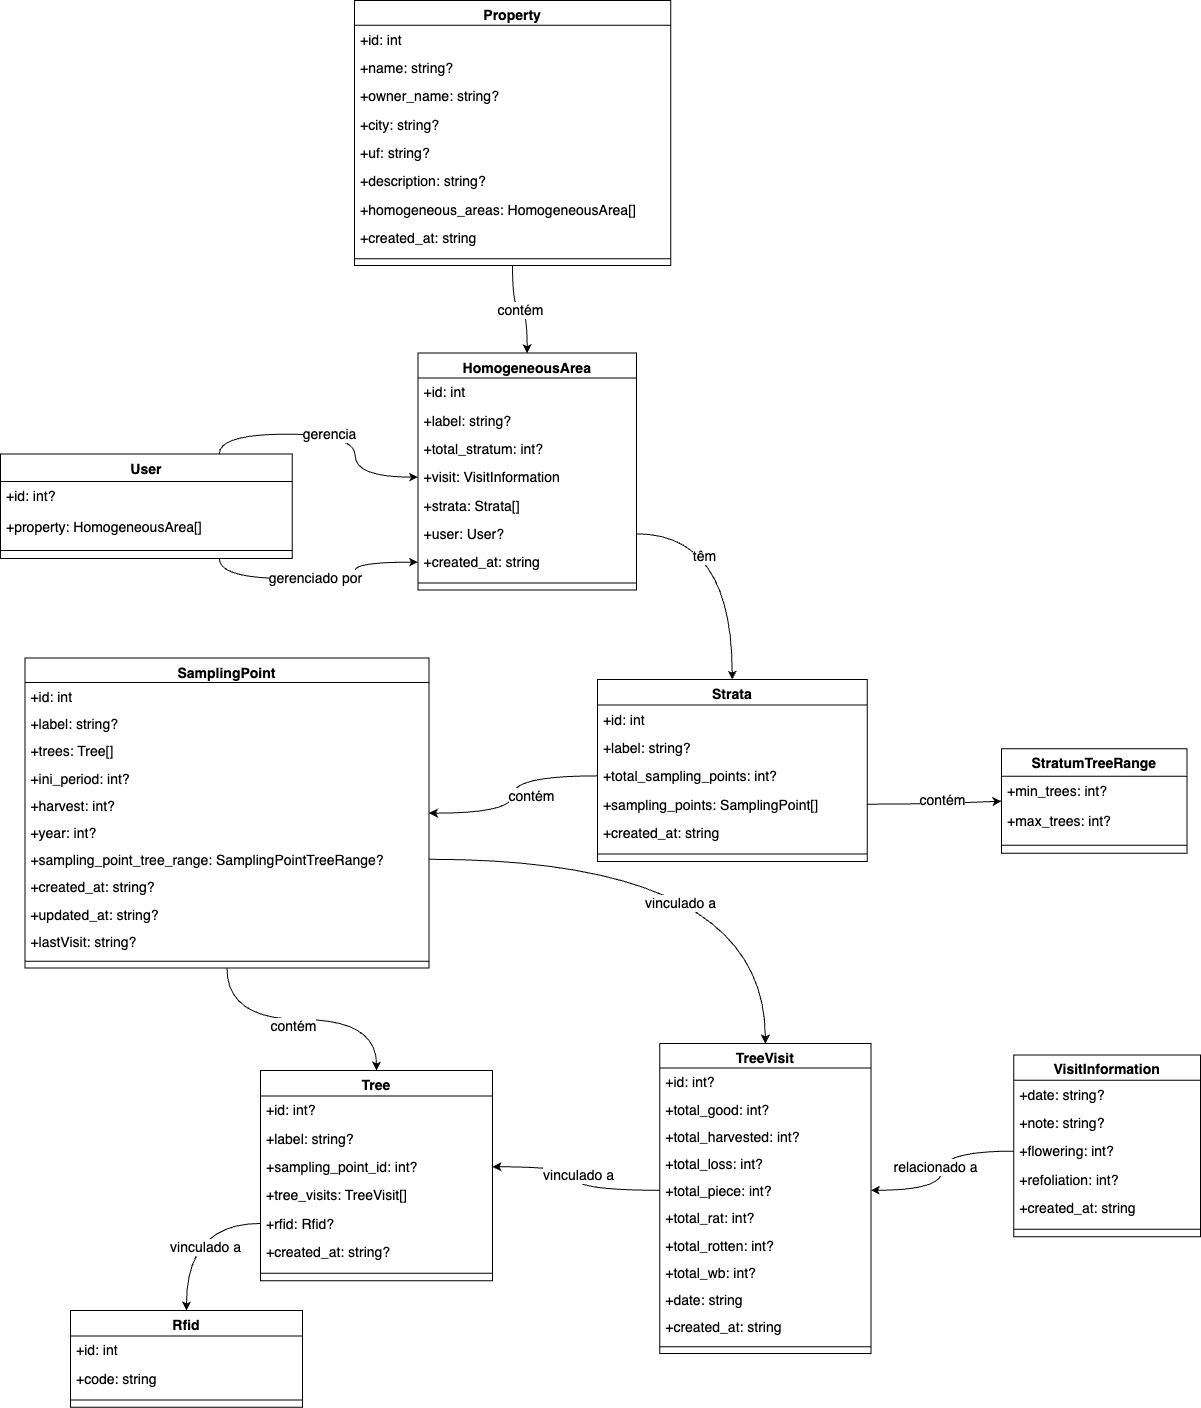
\includegraphics[width=\textwidth]{images/diagrams/class-diagram-p1.png}}
    \caption{Diagrama de classes das principais entidades do banco de dados \textit{offline}.}
    \label{fig:ClassDiagram01}
\end{figure}

\newpage 

A classe \textit{TreeVisit} armazena informações detalhadas sobre cada fruto, seguindo a metodologia estabelecida pela CEPLAC. No contexto das classes do \textit{RealmDB} implementadas no aplicativo, essa classe é modelada como é apresentado na Figura \ref{fig:ClassDiagram02}:

\begin{figure}[htb]
 \centering
 \frame{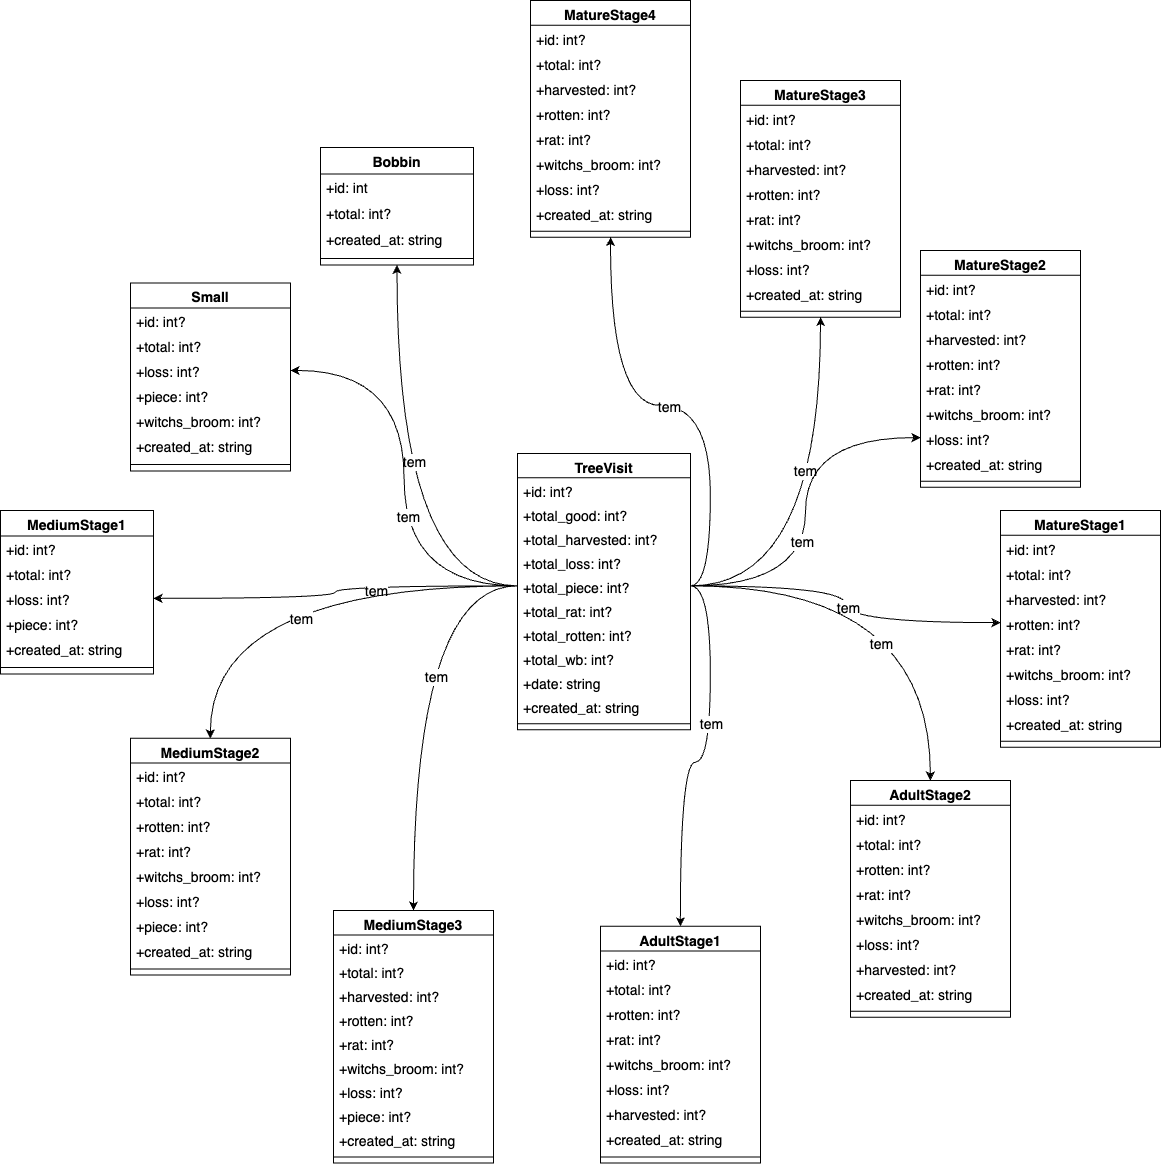
\includegraphics[width=\textwidth]{images/diagrams/class-diagram-p2.png}}
 \caption{Diagrama de classes do banco de dados \textit{offline} para os dados dos frutos.}
 \label{fig:ClassDiagram02}
\end{figure}

\newpage

\section{Integração com RFID}
A tecnologia RFID foi implementada para otimizar a identificação e monitoramento das árvores amostradas no ColetaCacau. Cada árvore recebe uma tag RFID, que contém um identificador único. Durante a coleta, o coletor utiliza o aplicativo para ler essas tags e associar os dados coletados à árvore correta.

\subsection{Processo de Implementação do RFID}
\begin{enumerate}
    \item \textbf{Leitura das Tags:} Um leitor RFID integrado ao dispositivo móvel lê a tag associada a uma árvore. O aplicativo, por meio de bibliotecas \textit{JavaScript} compatíveis com \textit{React Native}, interpreta essa leitura e exibe as informações da árvore diretamente na interface do usuário. Esse processo elimina a necessidade de o coletor identificar manualmente as árvores, reduzindo os erros e aumentando a precisão da coleta de dados. Um módulo nativo implementado em \textit{Kotlin} foi criado para atuar como um \textit{listener} verificando se existe algum dispositivo conectado ao celular e se este dispositivo é um leitor compátivel com a aplicação.

    \item \textbf{Associação com Dados Amostrais:} Assim que uma árvore é identificada via RFID, o aplicativo exibe as informações pré-existentes da árvore e permite que o coletor insira novos dados, como número de frutos ou condições da planta. Esses dados são armazenados localmente até que uma conexão à internet esteja disponível para sincronização com o servidor. O aplicativo identifica quando há uma conexão com internet e habilita o botão de envio de dados, que permite ao coletor enviar os dados que foram coletados.

    \item \textbf{Monitoramento de Erros com RFID:} A integração com o Sentry também monitora a estabilidade do sistema de leitura de tags RFID e de todo o aplicativo, garantindo que falhas sejam reportadas e corrigidas rapidamente, melhorando a confiabilidade do aplicativo.
\end{enumerate}

\section{Funcionalidades Desenvolvidas}

\subsection{Aprimoramento do Armazenamento \textit{Offline}}
A funcionalidade de coleta \textit{offline} do ColetaCacau, essencial para operação em áreas com baixa ou nenhuma conectividade e que já estava desenvolvida no aplicativo, foi aprimorada para oferecer maior segurança, integridade e eficiência no gerenciamento dos dados coletados. Nesta nova versão, o aplicativo se destaca por sua capacidade de armazenar informações localmente de maneira robusta, seguindo os padrões estabelecidos pela nova documentação do \textit{RealmDB}.

O \textit{RealmDB} foi aprimorado para oferecer desempenho superior no armazenamento local de dados, permitindo a coleta de grandes volumes de informações diretamente no dispositivo do coletor. Essa abordagem assegura que as informações sejam protegidas e prontamente disponíveis, mesmo em locais remotos.

\subsection{Gestão de Dados com \textit{Redux Toolkit}}
O \textit{Redux Toolkit} foi implementado para facilitar o gerenciamento de estado em todo o aplicativo, promovendo um fluxo de dados previsível e eficiente. Ele simplifica a definição de \textit{reducers}, \textit{actions} e a criação da \textit{store}, tornando a arquitetura do aplicativo mais robusta e escalável.

O \textit{Redux Persist} foi integrado ao sistema para garantir que o estado da aplicação seja preservado entre sessões, mesmo que o aplicativo seja fechado e reaberto. Isso assegura que os dados coletados no campo não sejam perdidos.

Atualmente, o ColetaCacau possui uma larga quantidade de dados, que é requisitada ao realizar o login no aplicativo. A utilização desta biblioteca alinhado ao uso do banco de dados \textit{offline} permite maior eficiência na manipulação destes dados.

\subsection{Monitoramento de Erros}
A integração com o \textit{Sentry} foi uma adição crucial ao sistema para garantir a estabilidade do aplicativo. O \textit{Sentry} monitora erros e exceções em tempo real, oferecendo relatórios detalhados sobre falhas que podem ocorrer no aplicativo, seja por incompatibilidade de dispositivos ou problemas de lógica de programação.

\begin{itemize}
    \item \textbf{Relatórios Automáticos:} Sempre que ocorre um erro no aplicativo, é gerado automaticamente um relatório que inclui detalhes técnicos sobre a falha, como a linha de código afetada, o tipo de erro e o dispositivo em que ocorreu.

    \item \textbf{Correção Proativa de Bugs:} Com base nos relatórios gerados por esta ferramenta, a equipe de desenvolvimento pode identificar rapidamente as falhas e liberar atualizações corretivas. Isso é especialmente importante para evitar a interrupção da coleta de dados em campo, onde o tempo é um recurso crítico.
\end{itemize}

\subsection{Atualização de Bibliotecas e \textit{Frameworks}}
Uma etapa essencial no aprimoramento do ColetaCacau foi a atualização do \textit{React Native} para a versão 0.76, descrita na documentação oficial do framework\footnote{\url{https://reactnative.dev/blog/2024/10/23/release-0.76-new-architecture}}. Essa atualização visou não apenas garantir compatibilidade com os sistemas operacionais móveis mais recentes, mas também trazer melhorias significativas na performance, segurança e eficiência do aplicativo.

Com a migração para a nova versão, houve uma redução substancial no tamanho final do aplicativo. Essa melhoria foi alcançada por meio de otimizações no código-base e pela remoção de dependências obsoletas, tornando o ColetaCacau mais leve e fácil de instalar, especialmente importante para usuários em áreas rurais com conectividade limitada. Além disso, o gerenciamento de memória foi aprimorado, o que resultou em uma navegação mais fluida e em uma melhor experiência para o usuário, mesmo em dispositivos com hardware modesto.

Outro benefício relevante foi o suporte ampliado para funcionalidades dos sistemas operacionais mais modernos, como melhorias na gestão de permissões e maior integração com bibliotecas essenciais, como o \textit{RealmDB} e o \textit{Redux}, garantindo a estabilidade e a robustez do aplicativo. Durante o processo de atualização, ajustes foram realizados no código para adaptar funcionalidades às mudanças da \textit{API} do \textit{React Native}, incluindo a substituição de métodos descontinuados e a reestruturação de componentes de interface. Esses ajustes asseguraram que o aplicativo estivesse alinhado às melhores práticas recomendadas.

Essas mudanças não apenas tornaram o aplicativo mais eficiente, mas também reforçaram sua estabilidade e capacidade de atender às necessidades dos coletores em campo, posicionando o ColetaCacau como uma solução tecnológica confiável e adaptada ao contexto da agricultura de precisão.

\section{Interface com o Usuário}
A interface do ColetaCacau foi projetada para ser simples e intuitiva, com uma navegação linear que facilita o uso em campo. O fluxo de navegação do aplicativo segue uma hierarquia clara, levando o usuário passo a passo desde o cadastro das propriedades até a coleta dos dados das árvores específicas.

\subsection{Fluxo de Navegação Linear do Aplicativo}
\begin{itemize}
    \item \textbf{Propriedades:} O processo começa com a listagem de propriedades cadastradas. Cada propriedade contém diversas áreas homogêneas. Cada propriedade é vinculada à um ou mais coletores.

    \item \textbf{Áreas Homogêneas:} Após selecionar uma propriedade, o usuário navega para as áreas homogêneas. Cada área homogênea é uma subdivisão que representa grandes regiões com características similares de solo, clima ou uso da terra.

    \item \textbf{Unidades Operacionais:} Dentro de cada área homogênea, há subdivisões chamadas de unidades operacionais, que representam setores menores, como blocos de uma fazenda. Ao selecionar uma unidade operacional, o usuário tem duas opções de navegação:
    \begin{itemize}
        \item \textbf{Dados da Prática:} O usuário pode optar por registrar dados gerais sobre o estado da área, como refoliação, floração, presença de pragas (como ratos e insetos), inundações, entre outros. Esses dados refletem a condição atual da área e ajudam no acompanhamento geral da plantação.

        \item \textbf{Pontos Amostrais:} Alternativamente, o usuário pode escolher navegar até os pontos amostrais, onde a coleta detalhada dos dados da árvore será realizada.
    \end{itemize}

    \item \textbf{Pontos Amostrais:} Ao acessar a lista de pontos amostrais, o coletor tem acesso às localizações específicas dentro das unidades operacionais, onde será realizada a coleta de dados mais detalhada. Cada ponto amostral contém várias árvores que são monitoradas individualmente.

    \item \textbf{Árvores:} Dentro de cada ponto amostral, o coletor verá a lista de árvores associadas. A integração com RFID facilita a identificação automática das árvores, permitindo que o coletor seja direcionado exatamente para a árvore correta, sem a necessidade de identificação manual.

    \item \textbf{Coleta dos Dados da Árvore:} Após a identificação da árvore, o usuário acessa a tela de coleta de dados específicos para cada árvore. Nessa tela, são registrados dados sobre o fruto do cacau, separados por estágios de desenvolvimento conforme o tempo (em dias) desde o último estágio de maturação.
    
    Estágios de Desenvolvimento do Fruto:
    \begin{itemize}
        \item 0 a 21 dias: Bilro
        \item 21 a 42 dias: Pequeno
        \item 42 a 63 dias: Médio
        \item 63 a 84 dias: Médio Estágio 2
        \item 84 a 105 dias: Médio Estágio 3
        \item 105 a 126 dias: Adulto
        \item 126 a 147 dias: Adulto Estágio 2
        \item 147 a 168 dias: Maduro
        \item 168 a 189 dias: Maduro Estágio 2
        \item 189 a 210 dias: Maduro Estágio 3
        \item Acima de 210 dias: Maduro Estágio 4
    \end{itemize}
\end{itemize}

Cada estágio representa uma fase específica no crescimento do fruto do cacau. O aplicativo permite que o coletor registre as informações de cada estágio, garantindo um acompanhamento detalhado e preciso da evolução da safra. Dados como quantidade de frutos, perdas e qualidade são registrados e vinculados ao estágio correspondente.

A arquitetura do ColetaCacau foi desenvolvida utilizando uma abordagem modular, garantindo que cada parte do sistema funcione de forma independente, mas integrando-se de maneira eficiente. O diagrama de componentes apresentado na Figura \ref{fig:ComponentsDiagram} ilustra como as diferentes partes do sistema, como o módulo de leitura de RFID, o gerenciamento de dados \textit{offline} e a interface do usuário, estão organizadas e interagem para garantir a funcionalidade completa do aplicativo.

\newpage 

\begin{figure}[htb]
    \centering
    \frame{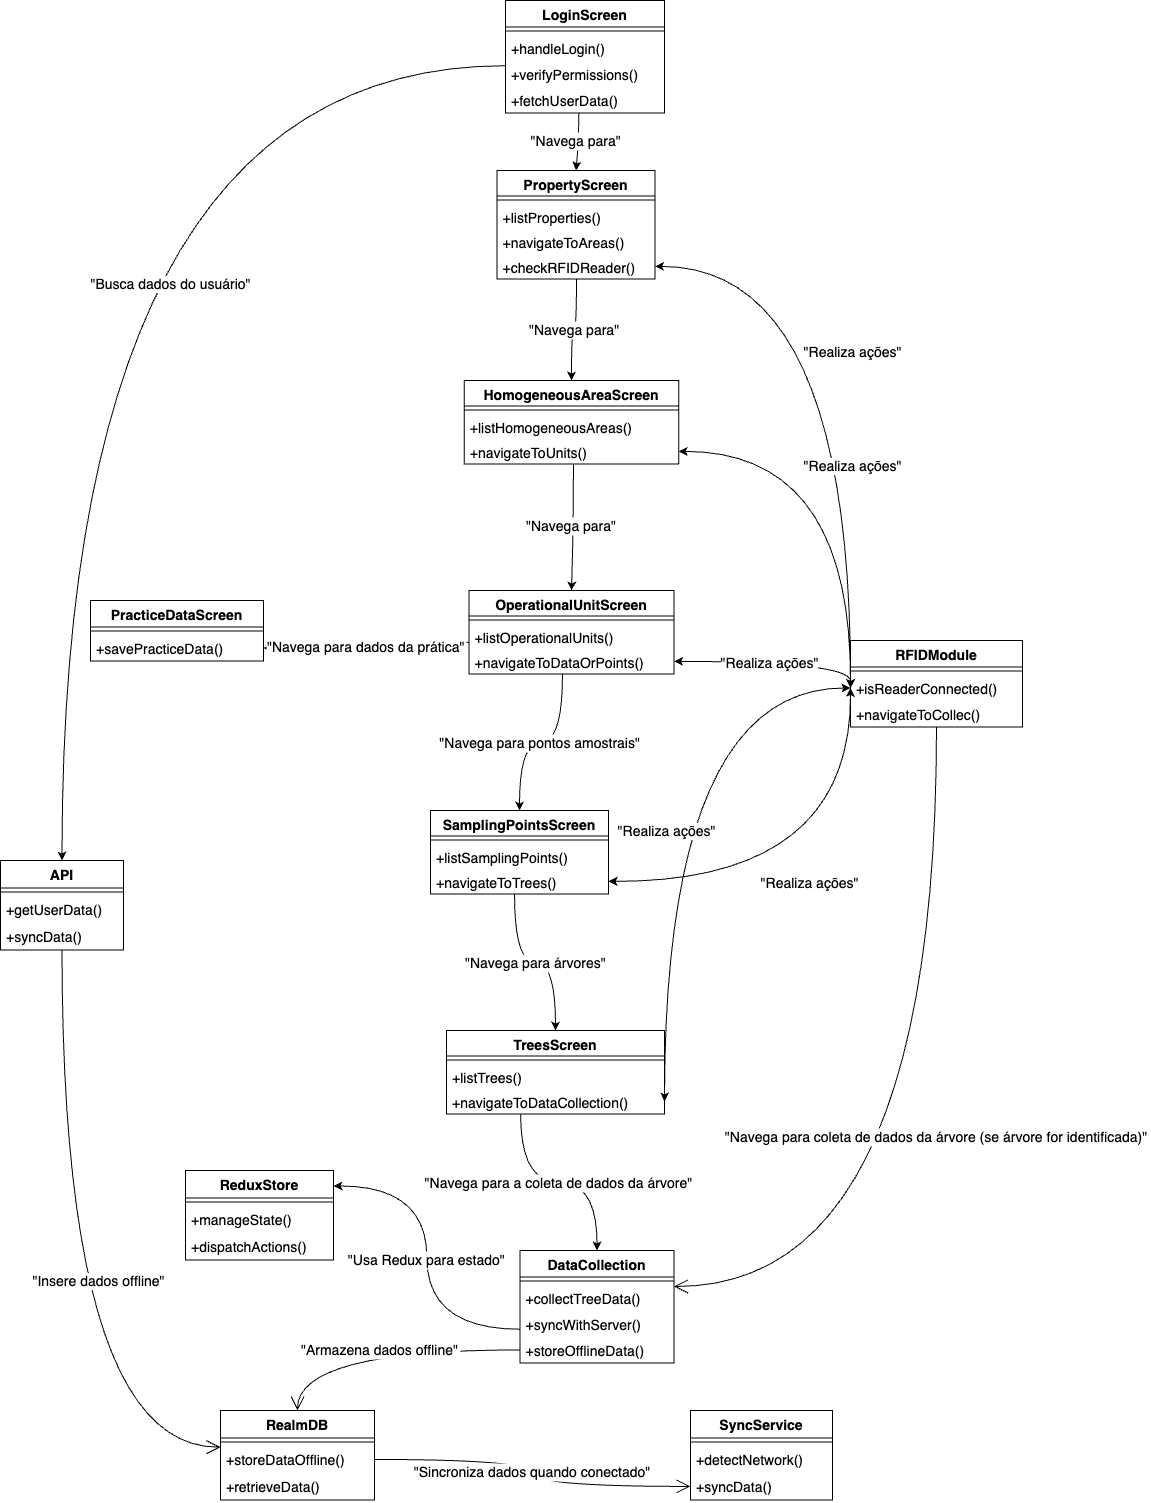
\includegraphics[width=\textwidth]{images/diagrams/components-diagram.png}}
    \caption{Diagrama de componentes.}
    \label{fig:ComponentsDiagram}
\end{figure}

\newpage

\subsection{\textit{Design} e Usabilidade}
O \textit{design} do ColetaCacau prioriza a simplicidade e a clareza. Cada passo do fluxo de navegação é apresentado de maneira clara e linear, o que facilita a operação por coletores que podem ter pouca familiaridade com tecnologia.

A interface também foi otimizada para garantir uma boa performance mesmo em dispositivos com \textit{hardware} limitado, uma realidade comum nas áreas rurais onde o aplicativo será utilizado.

\begin{itemize}
    \item \textbf{Telas organizadas:} As informações são exibidas em listas simples e fáceis de navegar, com botões de grande visibilidade que facilitam a interação.

    \item \textbf{Navegação intuitiva:} A hierarquia das telas segue a estrutura lógica da coleta de dados, o que facilita o uso em campo, mesmo em situações de pressão ou limitações de tempo.

    \item \textbf{Responsividade:} A interface foi projetada para ser responsiva e se adaptar a diferentes tamanhos de tela, garantindo uma experiência consistente tanto em smartphones quanto em tablets.
\end{itemize}

A Figura \ref{fig:CollectScreenTablet} mostra a visualização da tela de coleta de dados do cacau em um tablet, enquanto a Figura \ref{fig:CollectScreenPhone} demonstra a mesma tela adaptada para um smartphone, evidenciando a responsividade do \textit{design}.

\begin{figure}[H]
    \centering
    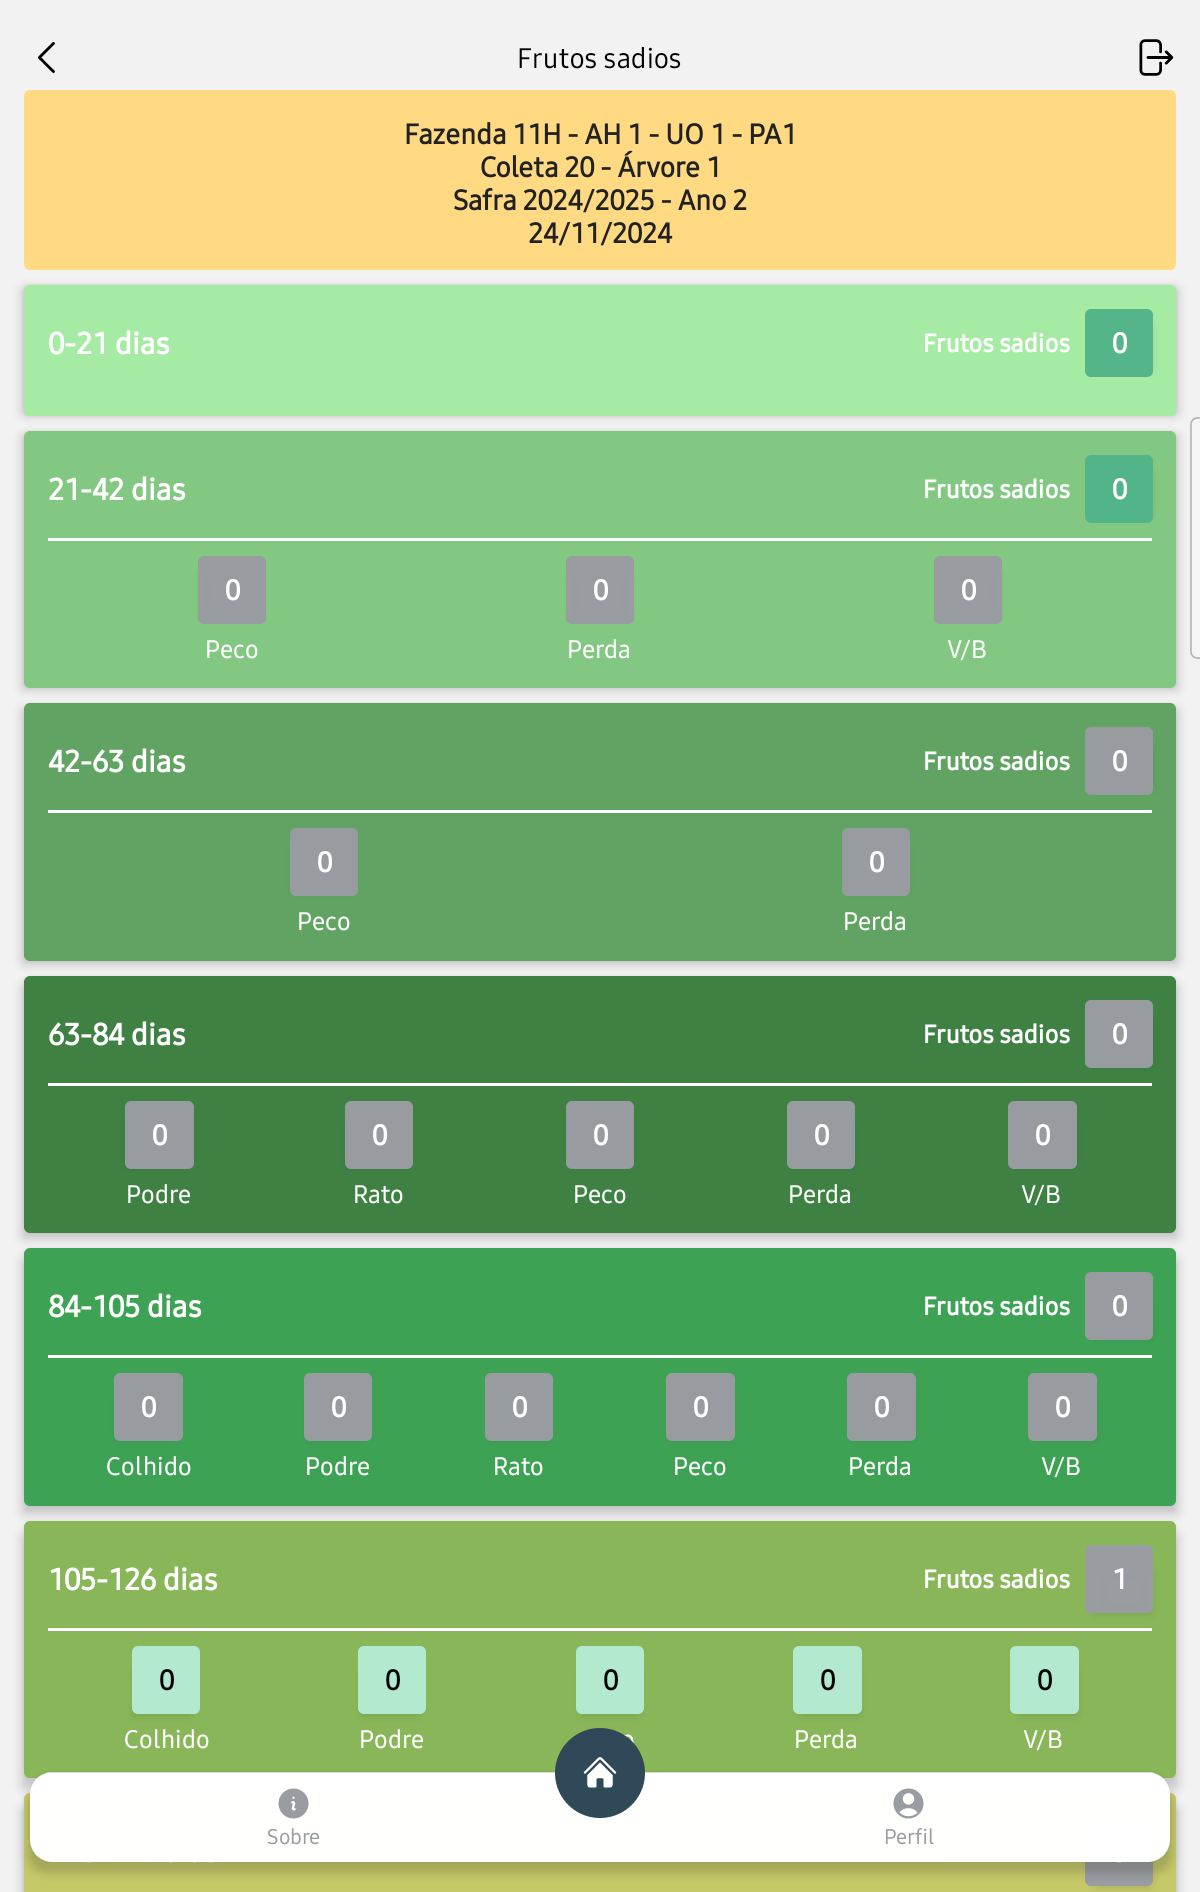
\includegraphics[width=0.4\textwidth]{images/app/collect-screen-tablet.png}
    \caption{Tela da coleta de dados em um \textit{tablet}.}
    \label{fig:CollectScreenTablet}
\end{figure}
\newpage
\begin{figure}[H]
    \centering
    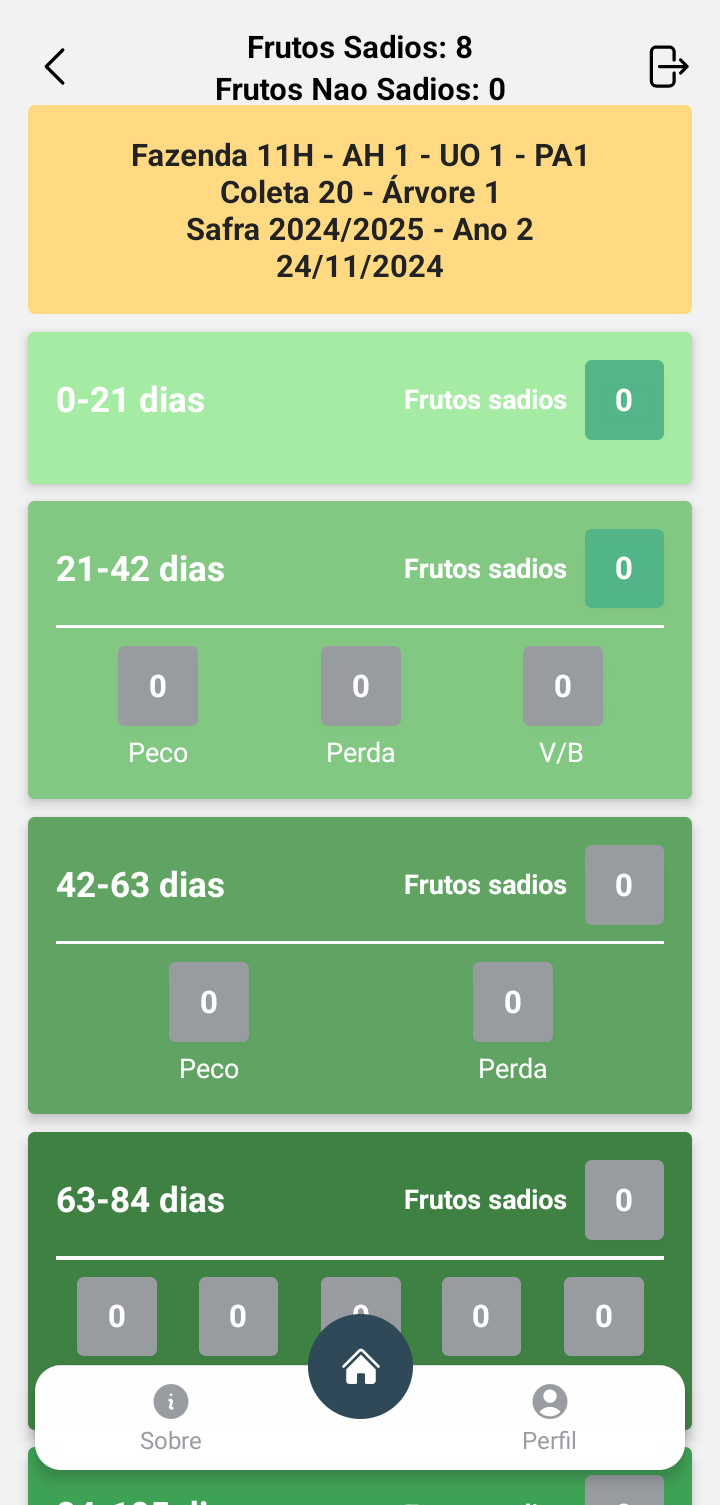
\includegraphics[width=0.4\textwidth]{images/app/collect-screen-phone.png}
    \caption{Tela da coleta de dados em um \textit{smartphone}.}
    \label{fig:CollectScreenPhone}
\end{figure}

Essa abordagem responsiva reforça o compromisso do ColetaCacau em oferecer uma experiência de usuário acessível e eficiente, independentemente do dispositivo utilizado no campo.

\subsection{Fluxo de Coleta e Operação}
A Figura \ref{fig:SequenceDiagram} representa o diagrama de sequência que descreve o processo de coleta de dados no ColetaCacau, desde o momento em que o coletor faz a leitura da tag RFID até o armazenamento dos dados localmente e a sincronização com o servidor. O diagrama detalha a interação entre os componentes principais do sistema — usuário, aplicativo, banco de dados \textit{offline} e servidor central —, mostrando o fluxo de operação e as etapas necessárias para garantir que os dados coletados sejam registrados corretamente e disponibilizados para análise.

\begin{figure}[htb]
 \centering
 \frame{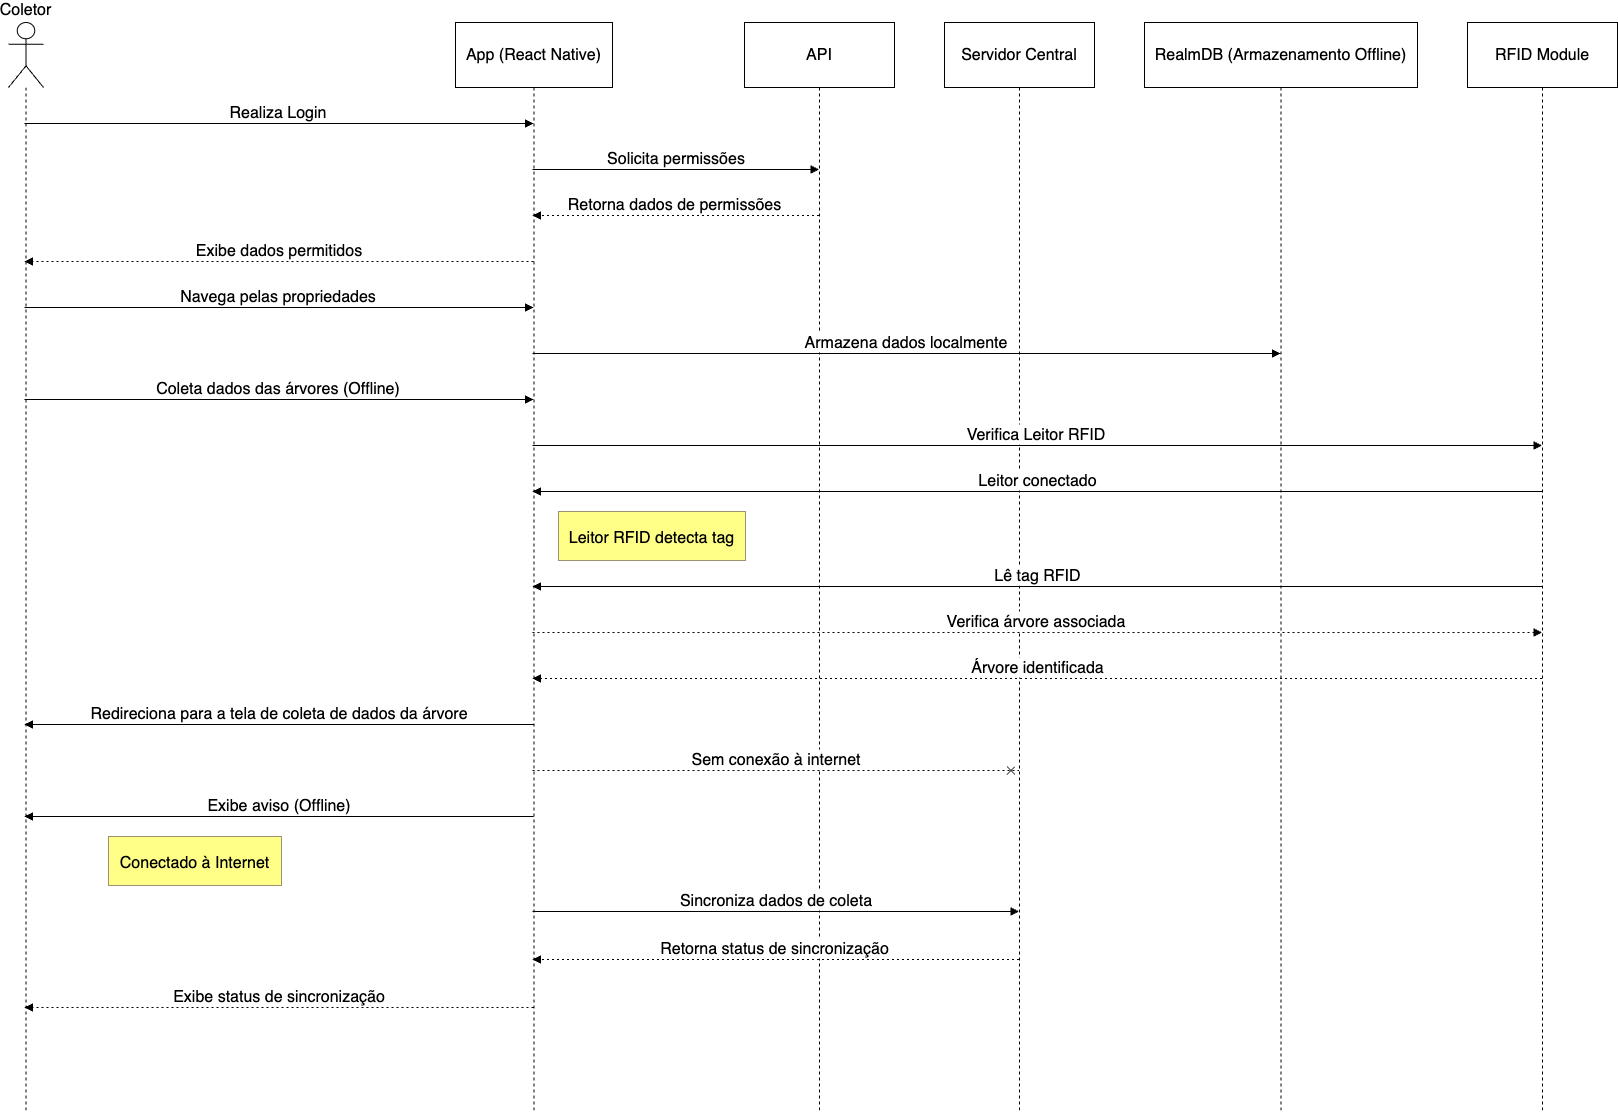
\includegraphics[width=\textwidth]{images/diagrams/sequence-diagram.png}}
 \caption{Diagrama de sequência.}
 \label{fig:SequenceDiagram}
\end{figure}

Para fornecer feedback visual ao coletor sobre a prontidão do aplicativo para realizar leituras de tags RFID, foi implementado um indicador no canto inferior direito de todas as telas de listagem. Esse indicador permite que o coletor saiba, em tempo real, se o leitor está ativo e pronto para captar informações de uma tag RFID, promovendo uma experiência mais fluida e intuitiva durante a coleta de dados.

A Figura \ref{fig:RfidReaderIndicator} ilustra os dois estados possíveis do indicador: no estado inativo, o leitor não está preparado para realizar a leitura; no estado ativo, o aplicativo está pronto para capturar as informações de uma tag, sinalizando de forma clara e acessível ao usuário. Essa funcionalidade reduz incertezas durante a operação e garante maior eficiência no processo de coleta.

\begin{figure}[H]
    \centering
    \begin{minipage}[b]{0.40\textwidth}
        \centering
        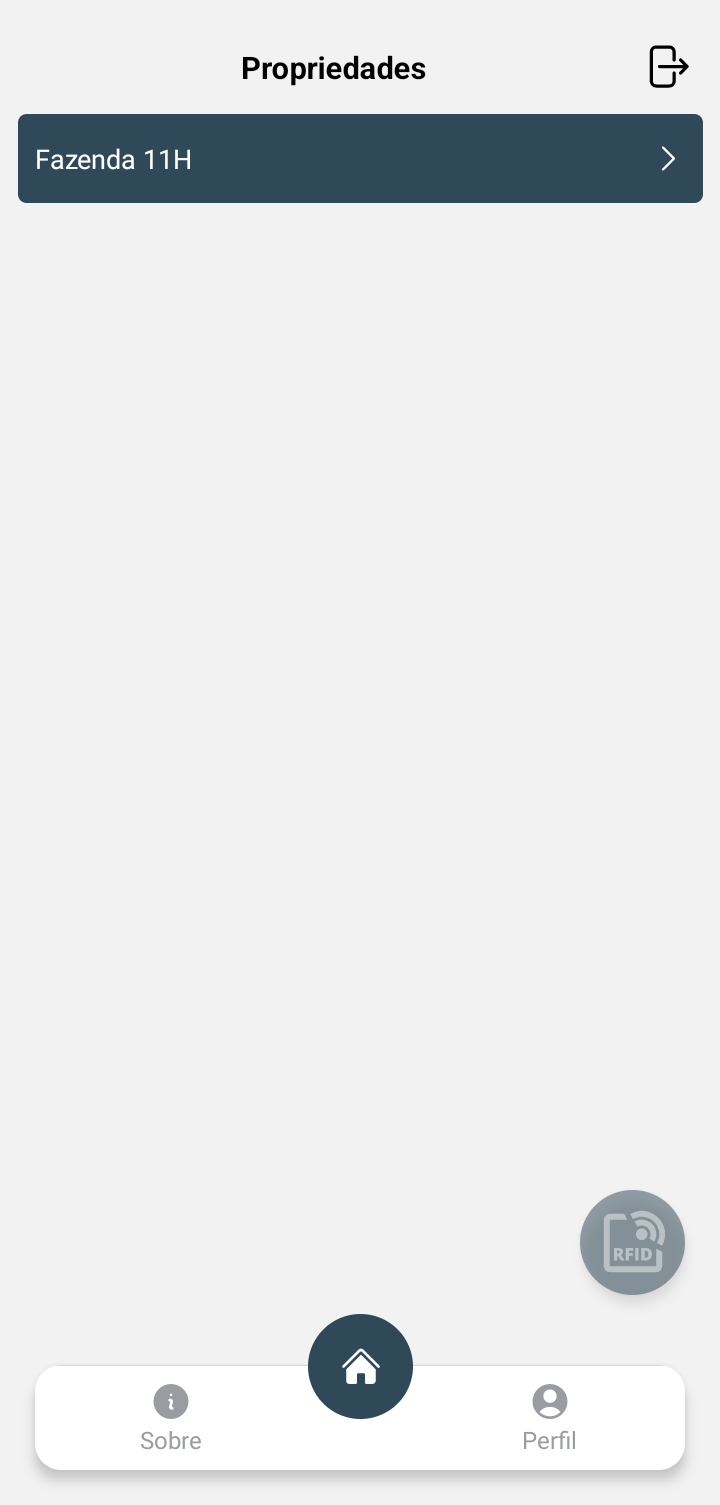
\includegraphics[width=\textwidth]{images/app/rfid-disabled.png}
        \caption*{(a) Indicador de leitura de tags em estado inativo.}
    \end{minipage}
    \hspace{5pt}
    \begin{minipage}[b]{0.40\textwidth}
        \centering
        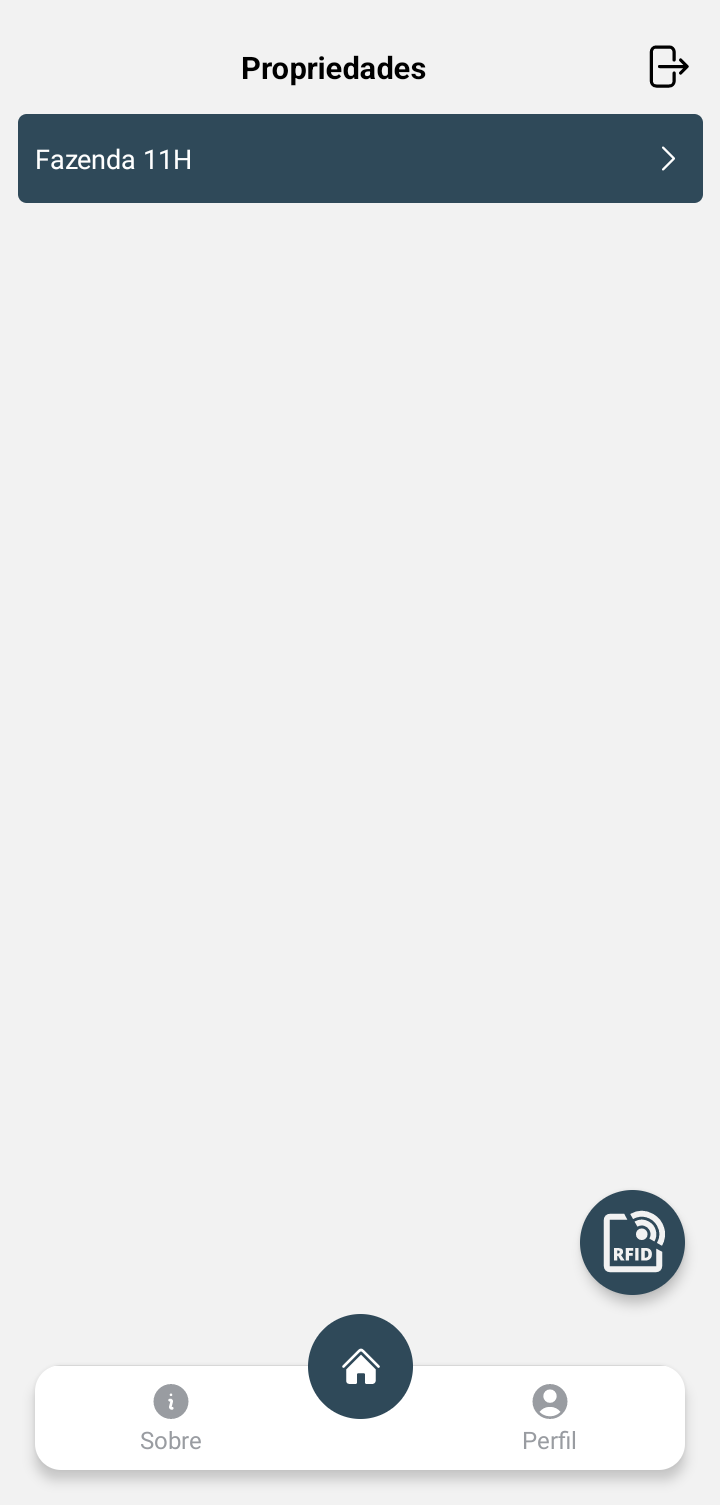
\includegraphics[width=\textwidth]{images/app/rfid-enabled.png}
        \caption*{(a) Indicador de leitura de tags em estado ativo.}
    \end{minipage}
    \hspace{5pt}
    
    \caption{Leitor RFID em dois estados: (a) Normal e (b) Ativo durante a leitura de uma tag.}
    \label{fig:RfidReaderIndicator}
\end{figure}

\newpage

\chapter{Implementação}

Neste Capítulo estão relacionadas as atualizações e melhorias feitas no aplicativo ColetaCacau para uso de RFID, bem como a especificação e arquitetura do sistema para atender esta nova demanda.

\section{Tecnologias Utilizadas}
O React Native foi escolhido para permitir o desenvolvimento multiplataforma, otimizando o tempo e os custos ao oferecer uma interface responsiva tanto para \textit{Android} quanto \textit{iOS} \cite{Erz2020IoTBM}. Para garantir o armazenamento local das informações coletadas no campo, mesmo sem conectividade, foi implementado o RealmDB, que sincroniza os dados assim que a internet se torna disponível \cite{Appiah2024PlanteSaineAA}.

O gerenciamento de estado global do aplicativo foi facilitado pelo Redux, garantindo consistência nos dados e fluidez na navegação \cite{Akter2023AgroBasedMA}. Além disso, o \textit{Sentry} foi integrado para monitoramento de erros em tempo real, promovendo estabilidade e confiabilidade do sistema, mesmo em cenários críticos de operação em campo.

\section{Leitor RFID Utilizado}
O leitor RFID utilizado no ColetaCacau é um modelo \textit{USB Contactless}, originalmente projetado para atuar como dispositivo de teclado \textit{HID} (\textit{Human Interface Device}), que facilita a integração e operação \textit{plug-and-play} com diversos sistemas, dispensando a necessidade de instalação de drivers complexos. Esse leitor, operando em frequência de 125KHz, possui uma antena de transceptor embutida, garantindo a captação de sinais mesmo sem linha direta de visão, característica essencial para o ambiente agrícola.

Compatível com padrões de cartões \textit{ISO14443A}, \textit{NTAG203}, \textit{Ultraleve}, \textit{Classic 1k (s50)} e \textit{Classic 4k (s70)}, o leitor oferece suporte a uma variedade de tags, possibilitando flexibilidade na escolha dos dispositivos de marcação. Ele é capaz de ler apenas o UID (Identificador Único) das tags, com saídas de 4 a 7 \textit{bytes} do número de série do chip, fornecendo informações essenciais para identificar cada árvore no sistema sem expor dados adicionais.

Alimentado via interface USB com tensão DC de 5V, o leitor facilita a implementação no campo, utilizando a alimentação diretamente do dispositivo ao qual está conectado, seja um dispositivo móvel ou um computador. Seu tempo de leitura de cartões é extremamente rápido, geralmente inferior a 100ms, o que permite que o coletor obtenha feedback instantâneo durante a coleta. Além disso, possui indicadores LED duplos, que informam o estado da leitura e facilitam o uso em condições de luz variável, frequentes em ambientes externos. Essas especificações do leitor tornam-no uma escolha eficiente e acessível para a implementação no ColetaCacau, contribuindo para a redução dos custos operacionais e proporcionando uma experiência de uso prática e robusta no campo.

Para os testes realizados tanto em campo quanto localmente, foram utilizados dois modelos de leitores RFID, ambos dentro das especificações descritas anteriormente. Esses modelos são ilustrados na Figura \ref{fig:RfidModels}, que apresenta as versões dos leitores \textit{USB} e \textit{USB-C}. 

\begin{figure}[H]
    \centering
    \begin{minipage}[b]{0.45\textwidth}
        \centering
        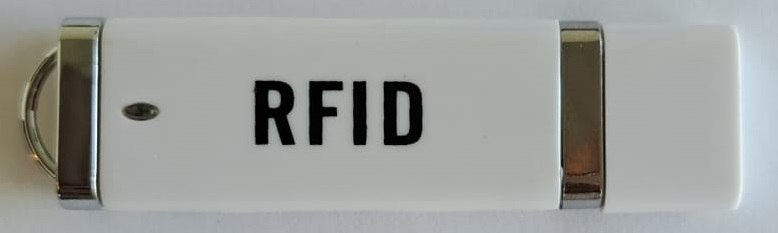
\includegraphics[width=\textwidth]{images/rfid/reader-01.jpg}
        \caption*{Leitor RFID - modelo USB.}
    \end{minipage}
    \hspace{5pt}
    \begin{minipage}[b]{0.35\textwidth}
        \centering
        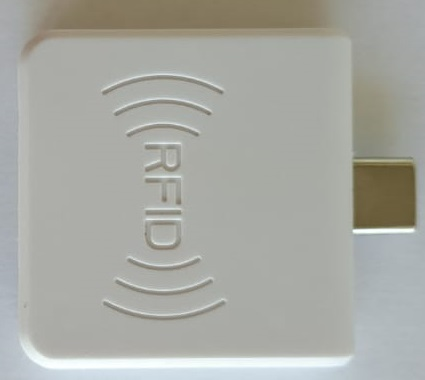
\includegraphics[width=\textwidth]{images/rfid/reader-02.jpg}
        \caption*{Leitor RFID - modelo USB-C.}
    \end{minipage}
    \hspace{5pt}
    
    \caption{Modelos de leitores RFID utilizados nos testes.}
    \label{fig:RfidModels}
\end{figure}

No aplicativo ColetaCacau, o leitor RFID é utilizado para captar as tags vinculadas a cada árvore no campo. Quando o coletor se aproxima da árvore equipada com a tag RFID, o sistema identifica automaticamente a tag lida e direciona o coletor para a árvore correspondente, integrando-se ao banco de dados \textit{RealmDB} para consultar e exibir as informações da árvore na interface. Esse processo automatizado elimina a necessidade de identificação manual, reduzindo significativamente o risco de erros operacionais e otimizando o tempo do coletor.

A programação do aplicativo permite que os sinais do leitor RFID sejam imediatamente associados ao banco de dados \textit{offline}, promovendo a sincronização entre a leitura em campo e o banco de dados do sistema, garantindo que o coletor visualize apenas a árvore correta sem qualquer ação manual adicional.

A Figura \ref{fig:RfidReader} ilustra o leitor RFID utilizado no ColetaCacau, destacando tanto o estado normal quanto o estado ativo durante a leitura de uma tag RFID. Essa visualização evidencia os indicadores LED duplos que fornecem uma resposta visual ao usuário, simplificando a operação em ambientes de campo e melhorando a eficiência do processo de coleta de dados.

\begin{figure}[H]
    \centering
    \begin{minipage}[b]{0.45\textwidth}
        \centering
        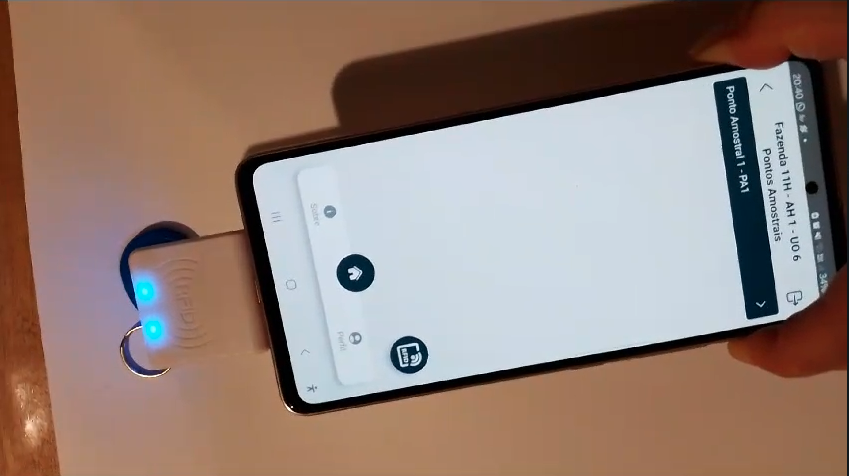
\includegraphics[width=\textwidth]{images/rfid/rfid-active.png}
        \caption*{(a) Estado Normal.}
    \end{minipage}
    \hspace{5pt}
    \begin{minipage}[b]{0.45\textwidth}
        \centering
        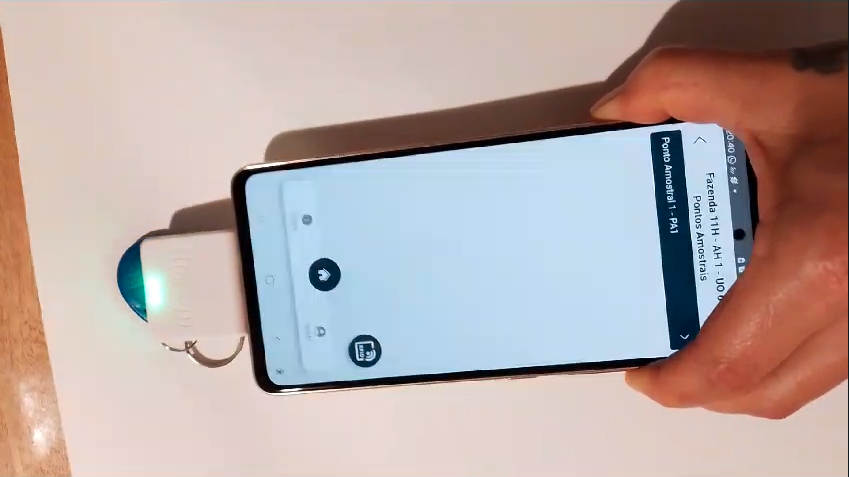
\includegraphics[width=\textwidth]{images/rfid/rfid-reading.png}
        \caption*{(b) Estado de Leitura.}
    \end{minipage}
    \hspace{5pt}
    
    \caption{Leitor RFID em dois estados: (a) Normal e (b) Ativo durante a leitura de uma tag.}
    \label{fig:RfidReader}
\end{figure}

\section{Tags RFID e Vinculação às Árvores}
No ColetaCacau, foram utilizadas tags RFID passivas de baixa frequência (12KHz) devido ao baixo custo de implementação e à durabilidade necessária para uso em campo, resistindo a intempéries e condições adversas. Cada tag RFID possui um identificador único constituído por uma sequência de 10 números aleatórios, garantindo a individualidade de cada árvore. Durante o cadastro, as tags são vinculadas a árvores específicas no sistema de gestão PlataformaCacau, permitindo que o aplicativo reconheça cada árvore automaticamente por meio da leitura da tag.

Cada código RFID é também vinculado à propriedade agrícola à qual a árvore pertence, assegurando que a integridade do banco de dados seja mantida e evitando duplicidades em diferentes propriedades. Essa organização fortalece o controle das informações, permitindo que as coletas subsequentes sejam precisas e garantindo que os coletores retornem sempre às mesmas árvores monitoradas.

A escolha por leitores e tags de baixa frequência reflete a necessidade de acessibilidade e sustentabilidade para uso em escala agrícola. A frequência de 12KHz reduz a susceptibilidade a interferências em campo, proporcionando uma leitura mais confiável, mesmo em ambientes adversos, e facilitando a implementação em várias propriedades sem a necessidade de elevados investimentos em infraestrutura.

Optou-se por não utilizar gravadores RFID de início, mantendo o foco na simplicidade e eficiência do sistema. Gravadores, que permitem a programação de tags, aumentariam tanto o custo quanto a complexidade do sistema, além de requerer uma infraestrutura mais robusta para regravação de dados nas tags, conforme necessário. Como cada árvore de uma propriedade é identificada unicamente.

Foi adotada, nesta fase do projeto, a estratégia de adquirir as tags gravadas de fábrica, por questões de custos e simplificação do processo. O fornecedor garante que a identificação é única, mas caso uma tag já cadastrada seja escaneada, o sistema alerta o usuário sobre a duplicidade, prevenindo inconsistências nos registros e mantendo a integridade dos dados coletados. O custo de cada tag já gravada ficou em torno de R\$2,00. O leitor de RFID entre R\$120,00 e R\$150,00.

Na Figura \ref{fig:RfidTags01} estão as primeiras tags RFID cadastradas e vinculadas no sistema, destacando a organização inicial e a vinculação prática com as árvores de cacau. Já a Figura \ref{fig:RfidTags02} exibe um conjunto adicional de tags RFID, mostrando a ampliação da aplicação do sistema para maior cobertura e controle no monitoramento.

\begin{figure}[H]
    \centering
    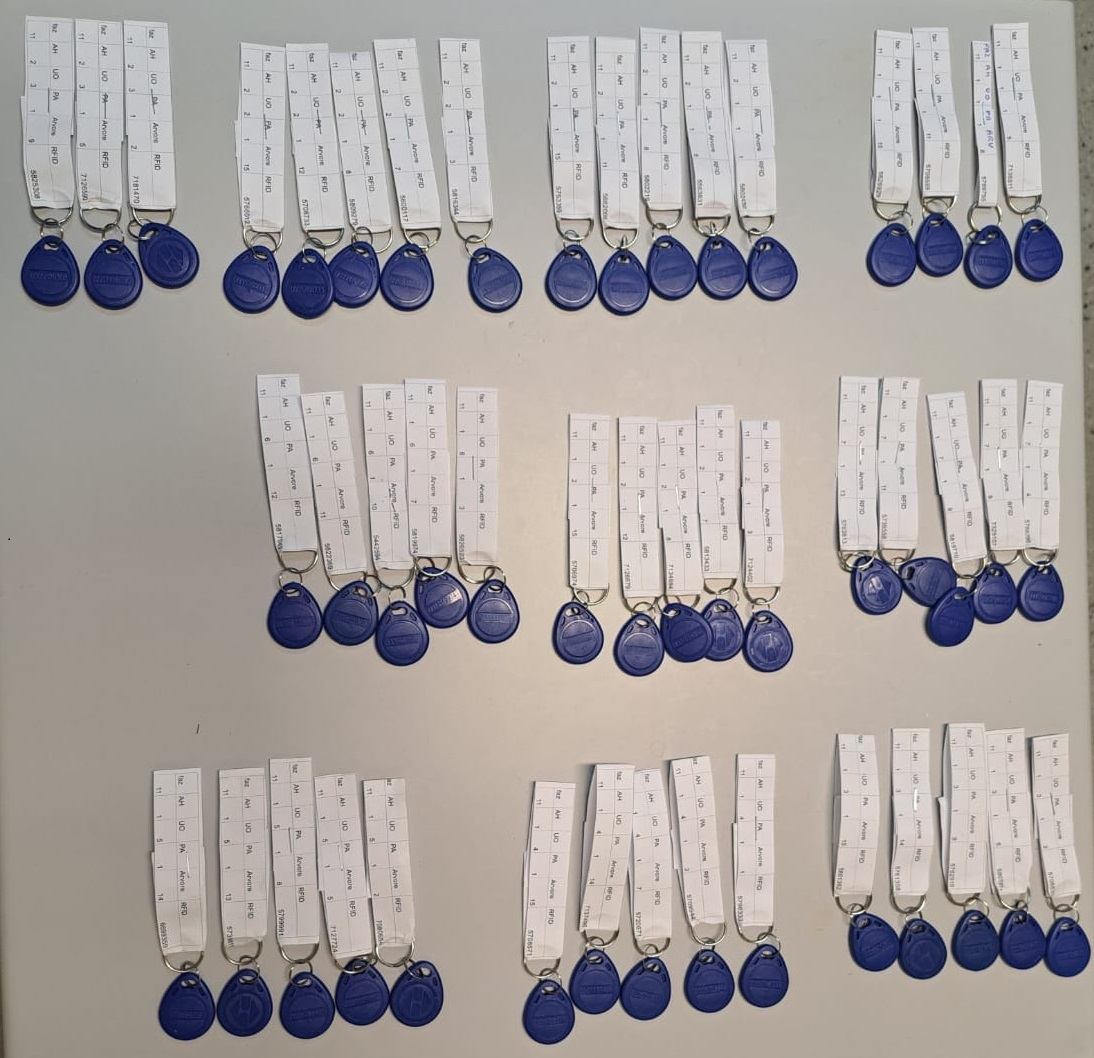
\includegraphics[width=0.6\textwidth]{images/rfid/rfid-tags-01.jpeg}
    \caption{Primeiras tags cadastradas e vinculadas (48 tags).}
    Autora: Marta M. Dornelles, 2024.
    \label{fig:RfidTags01}
\end{figure}

\begin{figure}[H]
    \centering
    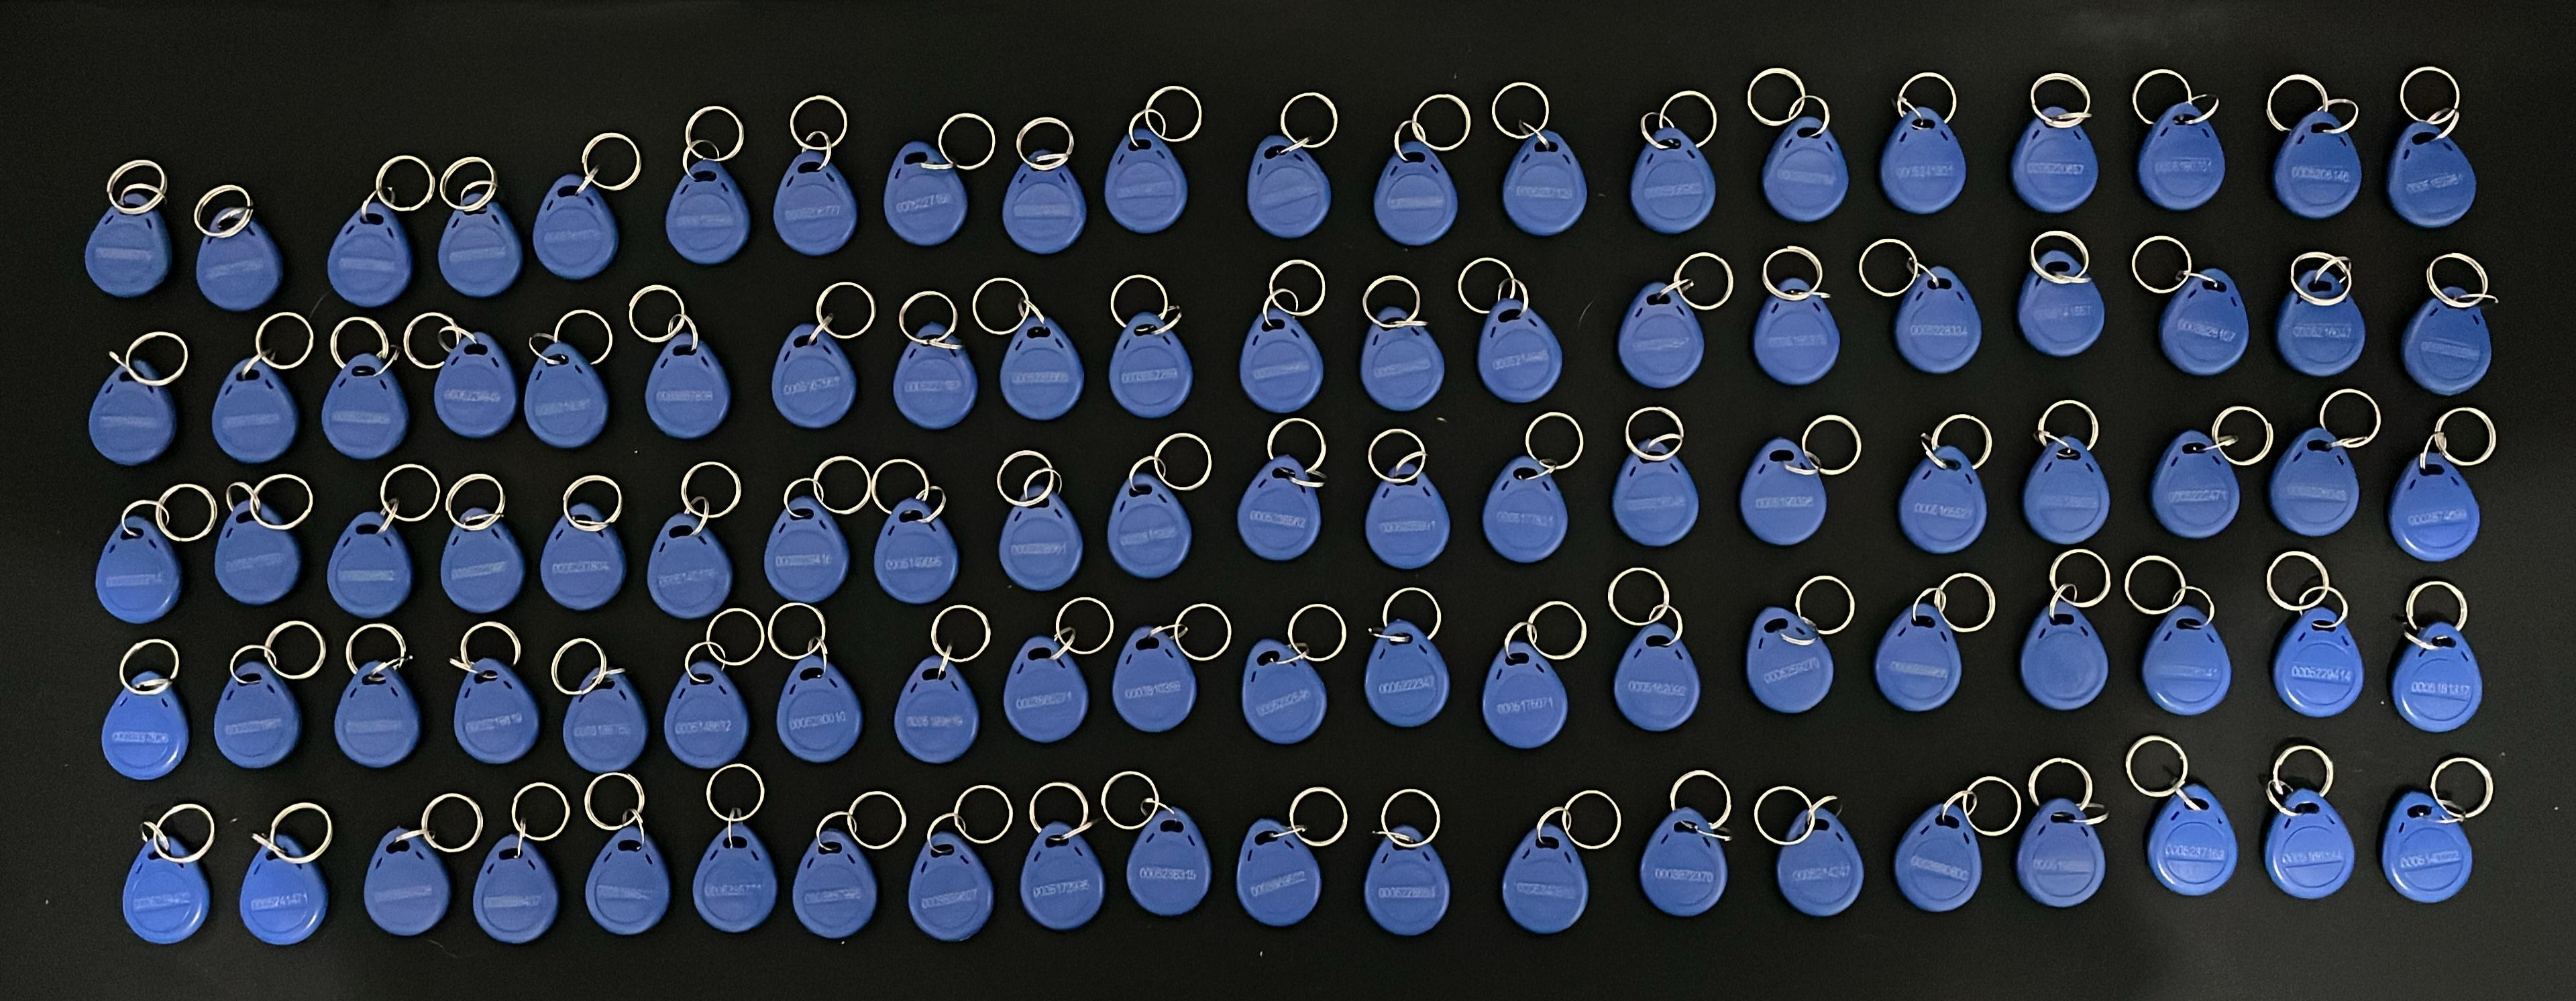
\includegraphics[width=0.8\textwidth]{images/rfid/rfid-tags-02.jpeg}
    \caption{Tags vinculadas posteriormente (92 tags).}
    Autor: Adriel F. da S. Oliveira, 2024.
    \label{fig:RfidTags02}
\end{figure}

Na Figura \ref{fig:RfidTag}, é apresentada uma visão detalhada da tag RFID utilizada, destacando o material e o código de 10 dígitos impresso na própria tag. Este código identifica exclusivamente cada árvore associada a uma propriedade no sistema ColetaCacau.

\begin{figure}[H]
    \centering
    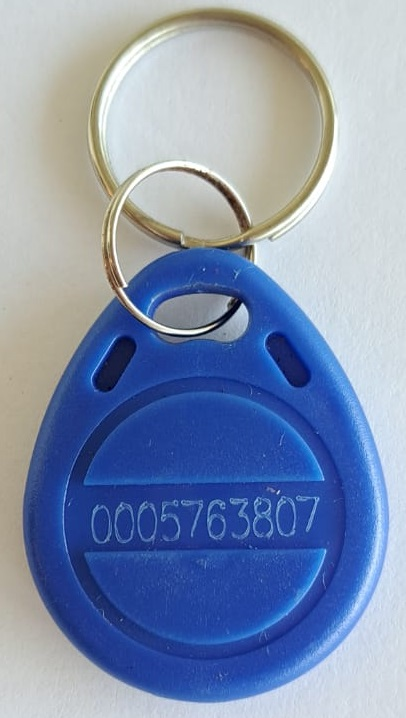
\includegraphics[width=0.4\textwidth]{images/rfid/tag.jpg}
    \caption{Tag RFID utilizada no ColetaCacau, com código impresso no material da tag.}
    \label{fig:RfidTag}
\end{figure}

\section{Módulo RFID Implementado}
O módulo RFID foi implementado com o objetivo de automatizar a identificação das árvores de cacau, melhorando a precisão e eficiência na coleta de dados em campo. Esse módulo é composto por uma integração entre o aplicativo móvel desenvolvido em React Native e um módulo nativo em Android, que gerencia a comunicação com o leitor RFID.

No React Native, o módulo de leitura de RFID utiliza a biblioteca \textit{NativeModules} para se comunicar diretamente com o hardware de leitura via USB. O leitor RFID, uma vez conectado ao dispositivo móvel, começa a capturar automaticamente as tags RFID associadas às árvores. Quando o coletor se aproxima de uma árvore equipada com a tag RFID, o sistema identifica a árvore e direciona o usuário para a tela correspondente no aplicativo, sem a necessidade de intervenção manual. Esse processo reduz significativamente os erros humanos, garantindo que os dados coletados sejam consistentes e mais precisos.

O \textit{layout} implementado oferece um campo de entrada para o código RFID e indicadores visuais claros sobre o status do leitor RFID (conectado ou desconectado). Quando uma tag RFID é lida com sucesso, o sistema fornece uma resposta visual imediata e direciona o coletor para o próximo passo no processo de coleta de dados.

A Figura \ref{fig:LayoutRfid} apresenta a tela do aplicativo, destacando a área de interação com a leitura das tags RFID.

\begin{figure}[H]
    \centering
    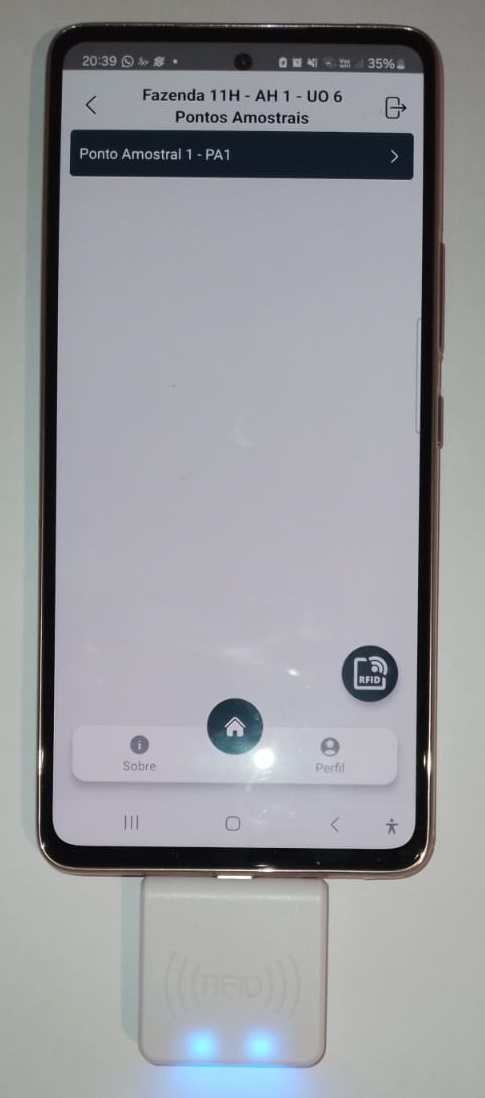
\includegraphics[width=0.35\textwidth]{images/rfid/phone.jpeg}
    \caption{Visulização completa do aplicativo com o leitor RFID}
    \label{fig:LayoutRfid}
\end{figure}

\section{Especificações}
O sistema ColetaCacau foi desenvolvido para otimizar a coleta de dados em campo, oferecendo funcionalidades avançadas que atendem às necessidades dos principais atores envolvidos no processo: os coletores e os gestores de fazendas. Abaixo, são detalhadas as especificações funcionais e não funcionais que guiaram o desenvolvimento do aplicativo.

Para garantir que as necessidades dos diferentes usuários sejam atendidas, o sistema ColetaCacau foi projetado com base em uma série de casos de uso. Os principais atores envolvidos são os coletores e os gestores de fazendas. Os coletores utilizam o aplicativo para registrar dados sobre as árvores e as áreas homogêneas, enquanto os gestores analisam esses dados para gerar relatórios de produtividade e acompanhar o progresso da safra. Na Figura \ref{fig:UseCasesDiagram} está a ilustração do diagrama de casos de uso com as principais interações desses atores com o sistema, detalhando as ações realizadas durante o processo de coleta de dados e análise.

\begin{figure}[H]
    \centering
    \frame{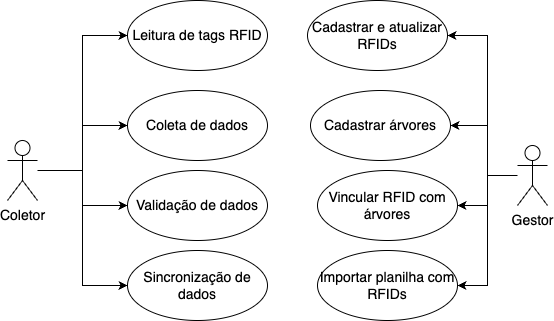
\includegraphics[scale=0.6]{images/diagrams/uc-diagram.png}}
    \caption{Diagrama de Casos de Uso.}
    \label{fig:UseCasesDiagram}
\end{figure}

\subsection{Requisitos Funcionais}
Os requisitos funcionais descrevem as funcionalidades que o sistema deve oferecer para atender às necessidades do usuário. No Quadro \ref{Tab:FunctionalReqs} a seguir estão descritos os requisitos funcionais (RF) atendidos pelo aplicativo.

\begin{quadro}[!htb]
    \centering
    \footnotesize
    \caption{Requisitos funcionais (RF).}
    \begin{tabular}{|c|p{4cm}|p{8cm}|}
        \hline
        \textbf{Identificação} & \centering\textbf{Nome} & \textbf{Descrição} \\
        \hline
        RF01          & Identificação Automática de Árvores         & O aplicativo deve ler as tags RFID das árvores e encaminhar o coletor automaticamente para tela da árvore respectiva.\\ \hline
        
        RF02          & Coleta \textit{Offline}          & O aplicativo deve funcionar completamente \textit{offline}, permitindo que os coletores registrem dados de campo sem necessidade de conexão com a internet. Os dados serão sincronizados posteriormente, quando a conexão estiver disponível. \\ \hline
        
        RF03          & Gerenciamento de Dados       &  O aplicativo deve possibilitar o armazenamento, edição e visualização dos dados coletados, permitindo que os usuários verifiquem informações sobre as árvores monitoradas e o progresso da safra.\\ \hline
        
        RF04          & Validação dos dados da coleta & O sistema deve incluir mecanismos para validar os dados inseridos pelos coletores, evitando a entrada de informações inconsistentes ou incompletas. Isso pode ser feito através de validações automáticas, que verificam se todos os campos obrigatórios foram preenchidos corretamente antes de permitir que os dados sejam salvos ou sincronizados com o servidor.\\ \hline
        
        RF05          & Cadastro de RFIDs & O sistema deve permitir que o gestor cadastre as tags RFID no banco de dados.\\ \hline
        
        RF06          & Vinculação de RFID com árvores & O sistema deve permitir que o gestor vincule cada RFID a uma árvore específica.\\ \hline

    \end{tabular}
    \label{Tab:FunctionalReqs}
    \fonte{o autor, 2024.}
\end{quadro}
\newpage

\subsection{Requisitos Não Funcionais}
Os requisitos não funcionais tratam das restrições e qualidades que o sistema deve atender. O Quadro \ref{Tab:NonFunctionalReqs} descreve os requisitos relacionados a certas restrições do sistema e aspectos de qualidade tanto do sistema quanto ao processo de desenvolvimento. 

\begin{quadro}[H]
	\centering
		\footnotesize
	\caption{Requisitos não funcionais (RNF).}
	\begin{tabular}{|c|p{8cm}|c|}
		\hline
		\textbf{Identificação} & \centering\textbf{Descrição} & \textbf{Classificação}\\
		\hline
		RNF01 & O aplicativo deve ser rápido e responsivo, mesmo em dispositivos móveis com capacidade limitada, garantindo uma experiência fluida ao usuário.   & Requisito de desempenho  \\ \hline
		
		RNF02 & Todas as informações coletadas devem ser armazenadas de forma segura e localmente, seguindo os padrões da Lei Geral de Proteção de Dados (LGPD).    & Requisito de segurança dos dados  \\ \hline
		
		RNF03 & O aplicativo deve ser compatível com as versões mais recentes dos sistemas operacionais Android e iOS. & Requisito de compatibilidade \\ \hline
		
		RNF04 & O aplicativo deve ser desenvolvido utilizando a o padrão de arquitetura MVVM (Movel, View, View-Model). & Requisito de implementação \\ \hline
		
		RNF05 & O \textit{design} do aplicativo deve ser simples e intuitivo, permitindo que os coletores, mesmo sem familiaridade com tecnologia, consigam utilizá-lo sem dificuldades. & Requisito de usabilidade \\ \hline
        
            RNF06 & O sistema deverá ser executado do Android 5.0 até o Android 14.  & Requisito de hardware \\ \hline

            RNF07 & O aplicativo deve ser capaz de realizar a leitura de tags no tempo limite de 1 segundo.  & Requisito de desempenho \\ \hline
	\end{tabular}
	\fonte{o autor, 2024.}
    \label{Tab:NonFunctionalReqs}
\end{quadro}

\section{Arquitetura do Sistema}
A arquitetura do sistema ColetaCacau, representada no diagrama C4 da Figura \ref{fig:C4Diagram}, foi cuidadosamente projetada para atender às necessidades de coleta de dados em ambientes rurais, garantindo eficiência e resiliência mesmo em condições de conectividade limitada. O sistema é composto por três camadas principais: interface, lógica de aplicação e dados. Além disso, inclui a PlataformaCacau, desenvolvida em \textit{Vue.js}, e uma API robusta construída em \textit{Laravel} para gerenciar e centralizar os dados coletados em campo.

\begin{figure}[H]
    \centering
    \frame{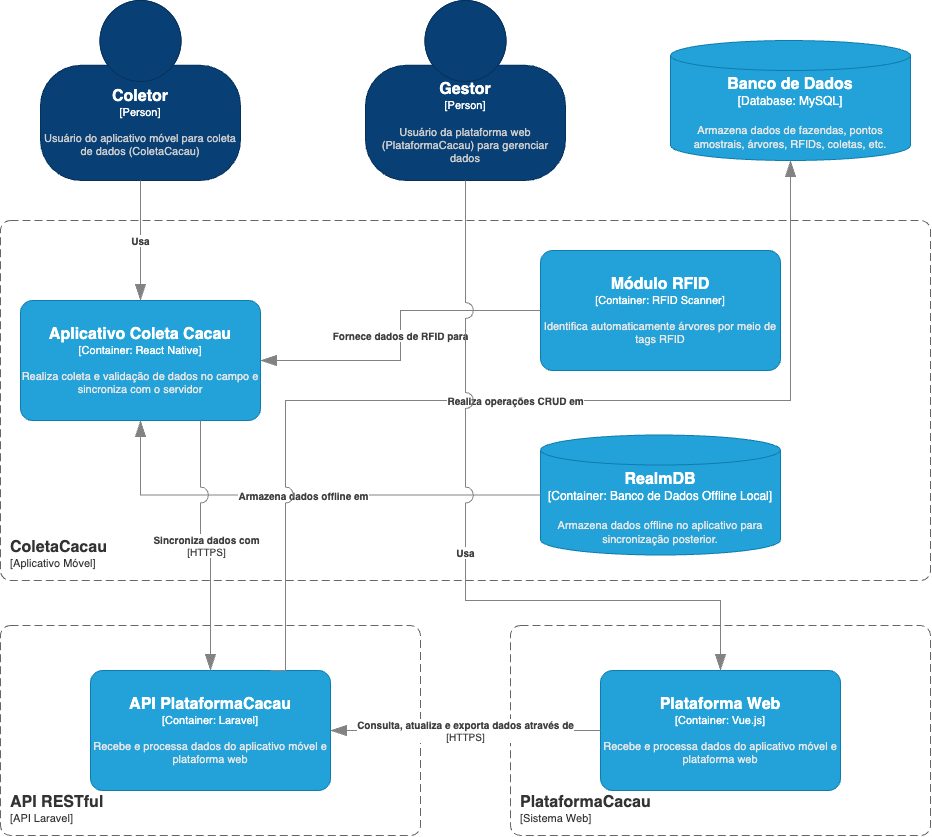
\includegraphics[width=\textwidth]{images/diagrams/c4-diagram.png}}
    \caption{Arquitetura do sistema ColetaCacau.}
    \fonte{o autor, 2024.}
    \label{fig:C4Diagram}
\end{figure}

A Camada de Interface (\textit{Front-End}) abrange duas plataformas: o aplicativo móvel, desenvolvido em \textit{React Native}, e a PlataformaCacau, uma interface web intuitiva e responsiva desenvolvida em \textit{Vue.js}. Enquanto o aplicativo é utilizado pelos coletores no campo para leitura de tags RFID e coleta de dados \textit{offline}, a PlataformaCacau é utilizada por gestores para o gerenciamento de propriedades, análise de dados e visualização de informações sincronizadas.

A Camada de Lógica de Aplicação gerencia o fluxo de informações entre a interface (móvel e web) e a API do \textit{back-end}. Essa camada inclui funcionalidades como leitura de tags RFID, sincronização \textit{offline}-\textit{online} e orquestração de dados coletados. A integração do \textit{Redux} no aplicativo assegura a consistência do estado global, enquanto a API, desenvolvida em \textit{Laravel}, proporciona uma comunicação segura e eficiente entre o \textit{front-end} e a base de dados centralizada.

A Camada de Dados (\textit{Back-End}) utiliza o \textit{RealmDB} no aplicativo móvel para armazenamento \textit{offline}, garantindo a operação em áreas remotas. A API \textit{Laravel} centraliza os dados sincronizados em um banco de dados relacional, permitindo análises avançadas e backup seguro. Assim, informações coletadas no campo pelo aplicativo são disponibilizadas para gestores na PlataformaCacau, promovendo uma visão holística e detalhada das operações.

\section{Fluxo de Coleta e Operação}
O fluxo operacional do aplicativo ColetaCacau com RFID envolve as seguintes etapas:

\begin{enumerate}
    \item \textbf{Cadastro de Árvores:} O usuário cadastra a fazenda e as árvores que serão monitoradas. Cada árvore recebe uma tag RFID, que será associada ao seu identificador no sistema web. Cada tag é única para a fazenda em que esta sendo realizada a vinculação.

    \item \textbf{Cadastro de RFID:} O usuário cadastra RFIDs com um código de até 10 dígitos númericos.

    \item \textbf{Leitura de Tags:} Ao chegar no campo, o coletor utiliza o aplicativo para ler as tags RFID das árvores. O aplicativo identifica automaticamente a árvore e exibe as informações de coleta associadas a ela.

    \item \textbf{Coleta de Dados:} O coletor preenche os dados de coleta, como o número de frutos, a condição da árvore e a qualidade da safra. Esses dados são armazenados localmente no RealmDB até que uma conexão à internet esteja disponível para sincronização.

    \item \textbf{Sincronização de Dados:} Quando o coletor retorna a uma área com conectividade, os dados armazenados \textit{offline} são automaticamente sincronizados com o servidor central, utilizando uma API segura.
\end{enumerate}


\chapter{Testes e resultados}

Neste capítulo estão relacionados os testes realizados para validar o funcionamento e a eficácia do aplicativo ColetaCacau, bem como os resultados obtidos após a implementação das funcionalidades de coleta de dados com RFID. A análise dos resultados foca na eficiência da coleta de dados em campo, redução de erros humanos, e na integração das funcionalidades com a plataforma web e a API.

\section{Testes Realizados}

Os testes foram realizados em três principais componentes do sistema: o aplicativo móvel (ColetaCacau), a plataforma web (PlataformaCacau) e a API. Abaixo estão descritos os principais cenários de teste e seus resultados:

\subsection{Testes no Aplicativo Móvel}

\subsubsection{Identificação Automática de Árvores com RFID}
Testou-se a leitura de tags RFID para garantir que o aplicativo reconhecesse automaticamente cada árvore. O teste validou a capacidade do aplicativo de vincular as árvores aos dados corretos da coleta, eliminando a necessidade de identificação manual.

A Figura \ref{fig:RfidTest01} ilustra como as tags RFID foram anexadas às árvores. Cada tag inicial contém informações visuais adicionais, como o nome da fazenda, área homogênea, unidade operacional e ponto amostral associados. Esses detalhes garantem que cada tag seja corretamente vinculada à árvore correspondente, promovendo precisão no processo de identificação e coleta. Foram testadas 140 tags, todas já anexadas às suas respectivas árvores. 

Para se ter ideia de custos, para cada área homogênea de cacau em uma propriedade são necessárias 35 plantas participantes da coleta. Esse valor pode aumentar um pouco a depender dos resultados observados. Uma área homogênea é aquela em que a produção de amêndoas é  próxima para todas as árvores, levando em consideração também outras variáveis como solo e tipo de cacau plantado. Geralmente, em 1 hectare são plantados aproximadamente 1000 plantas de cacau. 

\begin{figure}[H]
    \centering
    %\frame{
    \frame{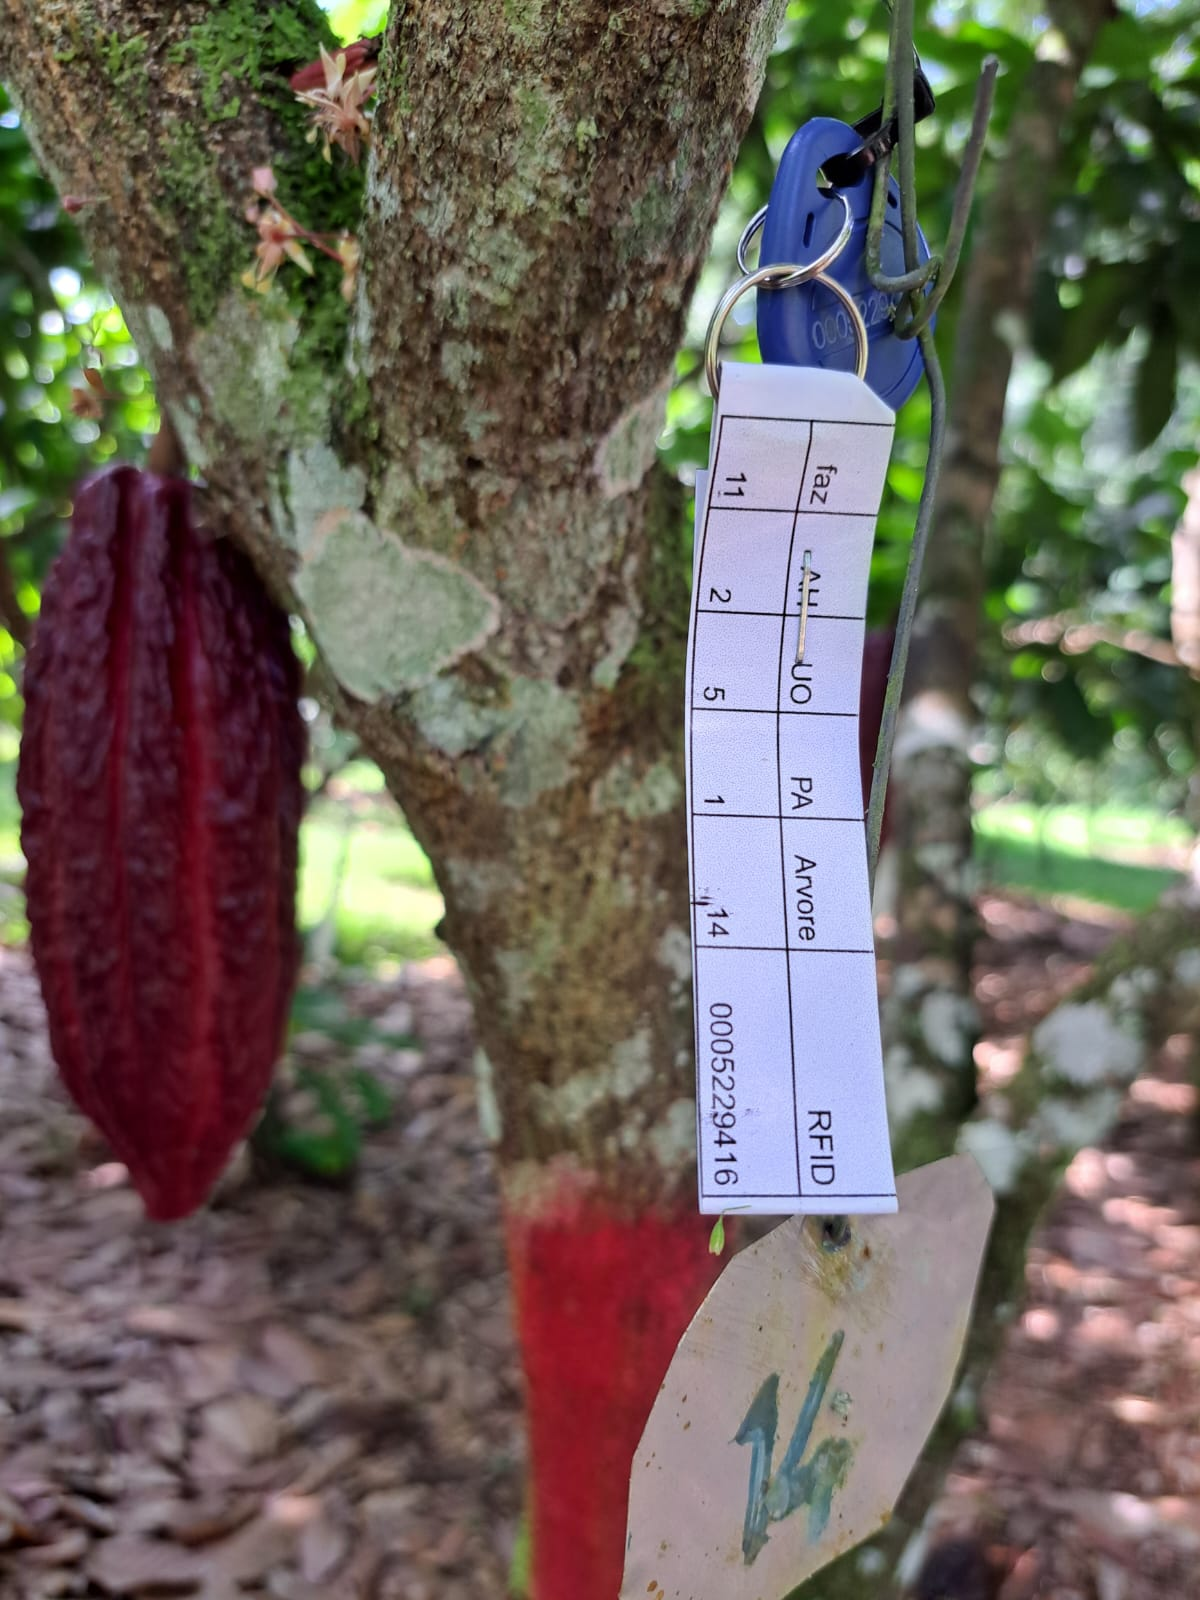
\includegraphics[width=0.4\textwidth]{images/rfid/rfid-test-01.jpeg}}\\
     \caption{Tag RFID vinculada a uma árvore, com informações adicionais para identificação.}
     Autora: Marta M. Dornelles, 2024.
    \label{fig:RfidTest01}
\end{figure}

Já a Figura \ref{fig:RfidTest02} demonstra o momento em que o aplicativo realiza a leitura da tag e consulta a base de dados \textit{offline}. Nesse processo, o sistema encaminha automaticamente o coletor para a tela correspondente à árvore lida, agilizando a navegação e garantindo a consistência na coleta de dados.

\begin{figure}[htb]
    \centering
    \frame{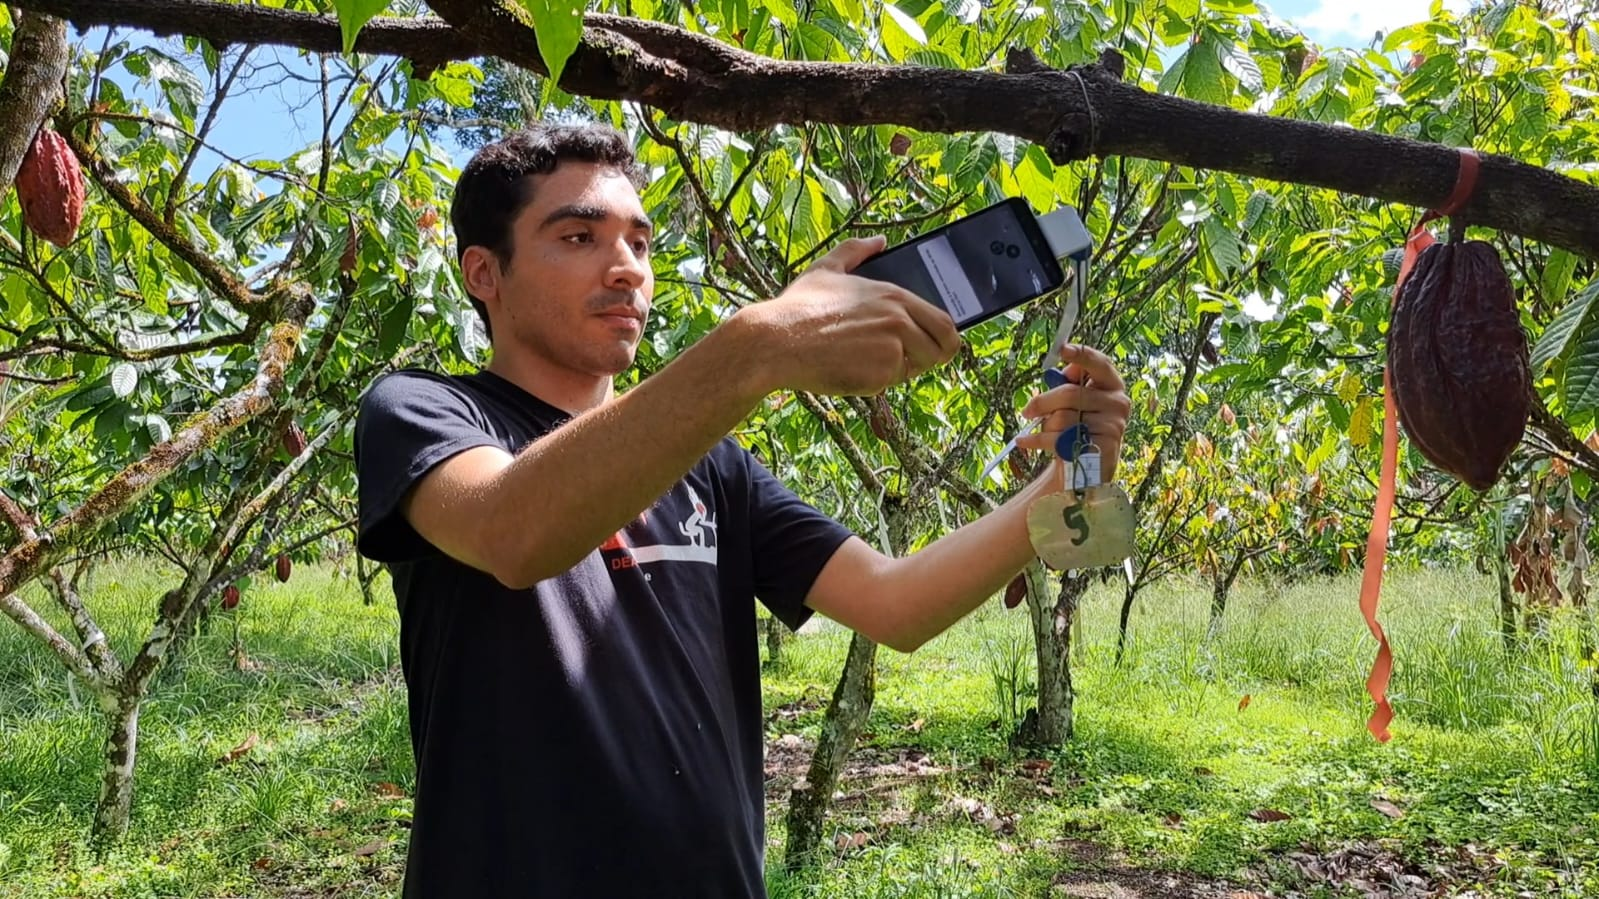
\includegraphics[width=0.7\textwidth]{images/rfid/rfid-test-02.jpeg}}
        \caption{Tela de consulta à tag RFID e direcionamento para os dados correspondentes da árvore.}
     Autora: Marta M. Dornelles, 2024.
    \label{fig:RfidTest02}
\end{figure}

\subsubsection{Coleta \textit{Offline} e Sincronização de Dados}
Avaliou-se a capacidade do aplicativo de coletar dados \textit{offline} e sincronizá-los com o servidor quando uma conexão fosse restabelecida. O teste confirmou que os dados coletados em campo são armazenados no banco de dados local (\textit{RealmDB}) e sincronizados corretamente.

\subsubsection{Validação de Dados da Coleta}
Realizou-se uma série de testes para validar a entrada de dados, assegurando que o aplicativo impedisse o envio de dados incompletos ou inconsistentes. O teste verificou o preenchimento correto de todos os campos obrigatórios antes de salvar ou sincronizar os dados.

\subsection{Testes na Plataforma Web}
\subsubsection{Cadastro e Atualização de RFIDs}
Testou-se o fluxo de cadastro e atualização de códigos RFID através da interface web, garantindo que o gestor pudesse criar e modificar os códigos das tags com facilidade e precisão. Foram feitas validações para não permitir inclusão de códigos de tags que já existissem em uma determinada propriedade vinculada àquele usuário.

\subsubsection{Vinculação de RFIDs com Árvores}
Validou-se o processo de vinculação dos RFIDs cadastrados às árvores específicas, tanto no cadastro inicial quanto na atualização de informações. Os testes garantiram que o código RFID correto fosse associado à árvore correspondente, permitindo a identificação precisa no campo.

\subsubsection{Listagem e Edição de Árvores}
A funcionalidade de listagem e edição de árvores foi testada para garantir que as informações fossem exibidas de maneira clara, permitindo ao gestor atualizar os dados conforme necessário.

\subsection{Testes na API e Banco de Dados}
\subsubsection{Criação e Atualização de RFIDs}
Testou-se os \textit{endpoints} de criação, atualização, listagem, visualização, associação e desassociação de RFIDs com árvores, garantindo que o sistema mantivesse a integridade dos dados e refletisse as alterações na plataforma web e no aplicativo.

\subsubsection{Exportação dos Dados da Coleta}
Avaliou-se a exportação dos dados coletados, incluindo o campo RFID vinculado às árvores. O teste confirmou que os dados exportados incluíam as informações corretas, facilitando a análise pelos gestores.

\section{Resultados Obtidos}
A implementação da tecnologia RFID no processo de coleta de dados representou um marco importante na eficiência e na precisão das operações em campo. Antes da adoção dessa tecnologia, os coletores enfrentavam desafios significativos na localização das árvores, o que envolvia um padrão de deslocamento confuso e ineficaz, frequentemente descrito como um trajeto em “zig-zag”. Esse método, além de consumir mais tempo e energia, contribuía para o aumento de erros na identificação das árvores e na coleta de informações, comprometendo a confiabilidade dos dados.

Com a introdução das tags RFID, cada árvore passou a ser identificada de forma única e automática, eliminando a necessidade de movimentações desordenadas. Agora, os coletores conseguem localizar rapidamente as árvores marcadas, utilizando leitores RFID que fornecem informações precisas e em tempo real. Essa mudança resultou em uma significativa economia de tempo, permitindo que o foco dos coletores fosse direcionado à coleta de dados propriamente dita, sem distrações ou esforços desnecessários.

Os benefícios dessa abordagem vão além da economia de tempo. A automatização do processo trouxe uma redução considerável dos erros humanos, anteriormente comuns devido à identificação manual ou a métodos visuais imprecisos. Com o RFID, a identificação das árvores tornou-se padronizada e consistente, promovendo maior confiabilidade e uniformidade nos dados coletados. Essa melhoria não apenas elevou a qualidade do trabalho realizado, mas também contribuiu para análises mais precisas e decisões informadas em etapas subsequentes do projeto.

Outro impacto relevante foi o aumento da produtividade dos coletores. Antes da implementação do RFID, o desgaste físico e mental causado pela movimentação desordenada e pela dificuldade em localizar as árvores comprometia o desempenho da equipe. Agora, com a otimização dos trajetos e a simplificação do processo, os coletores podem realizar suas tarefas com mais agilidade e menos esforço, gerando um ambiente de trabalho mais eficiente e satisfatório.

Além disso, a utilização do RFID trouxe ganhos indiretos, como a redução do custo operacional, uma vez que o tempo economizado por coleta possibilita a execução de mais tarefas em menos tempo. A confiabilidade nos dados também facilita a integração com sistemas de análise automatizada, como ferramentas de \textit{big data} ou inteligência artificial, abrindo caminho para futuras inovações no gerenciamento de informações.

\section{Seções de Imagens}
Para ilustrar o funcionamento do ColetaCacau e as funcionalidades implementadas na plataforma web e no aplicativo móvel, a seguir são apresentadas capturas de tela detalhando as principais interfaces e fluxos do sistema.

\subsection{Imagens da Plataforma Web}

\subsubsection{Tela de Listagem de RFIDs}
A Figura \ref{fig:ListRfid} exibe todos os RFIDs cadastrados no sistema, permitindo que o gestor visualize rapidamente os códigos e os associe às árvores de maneira eficiente.

\begin{figure}[H]
    \centering
    \frame{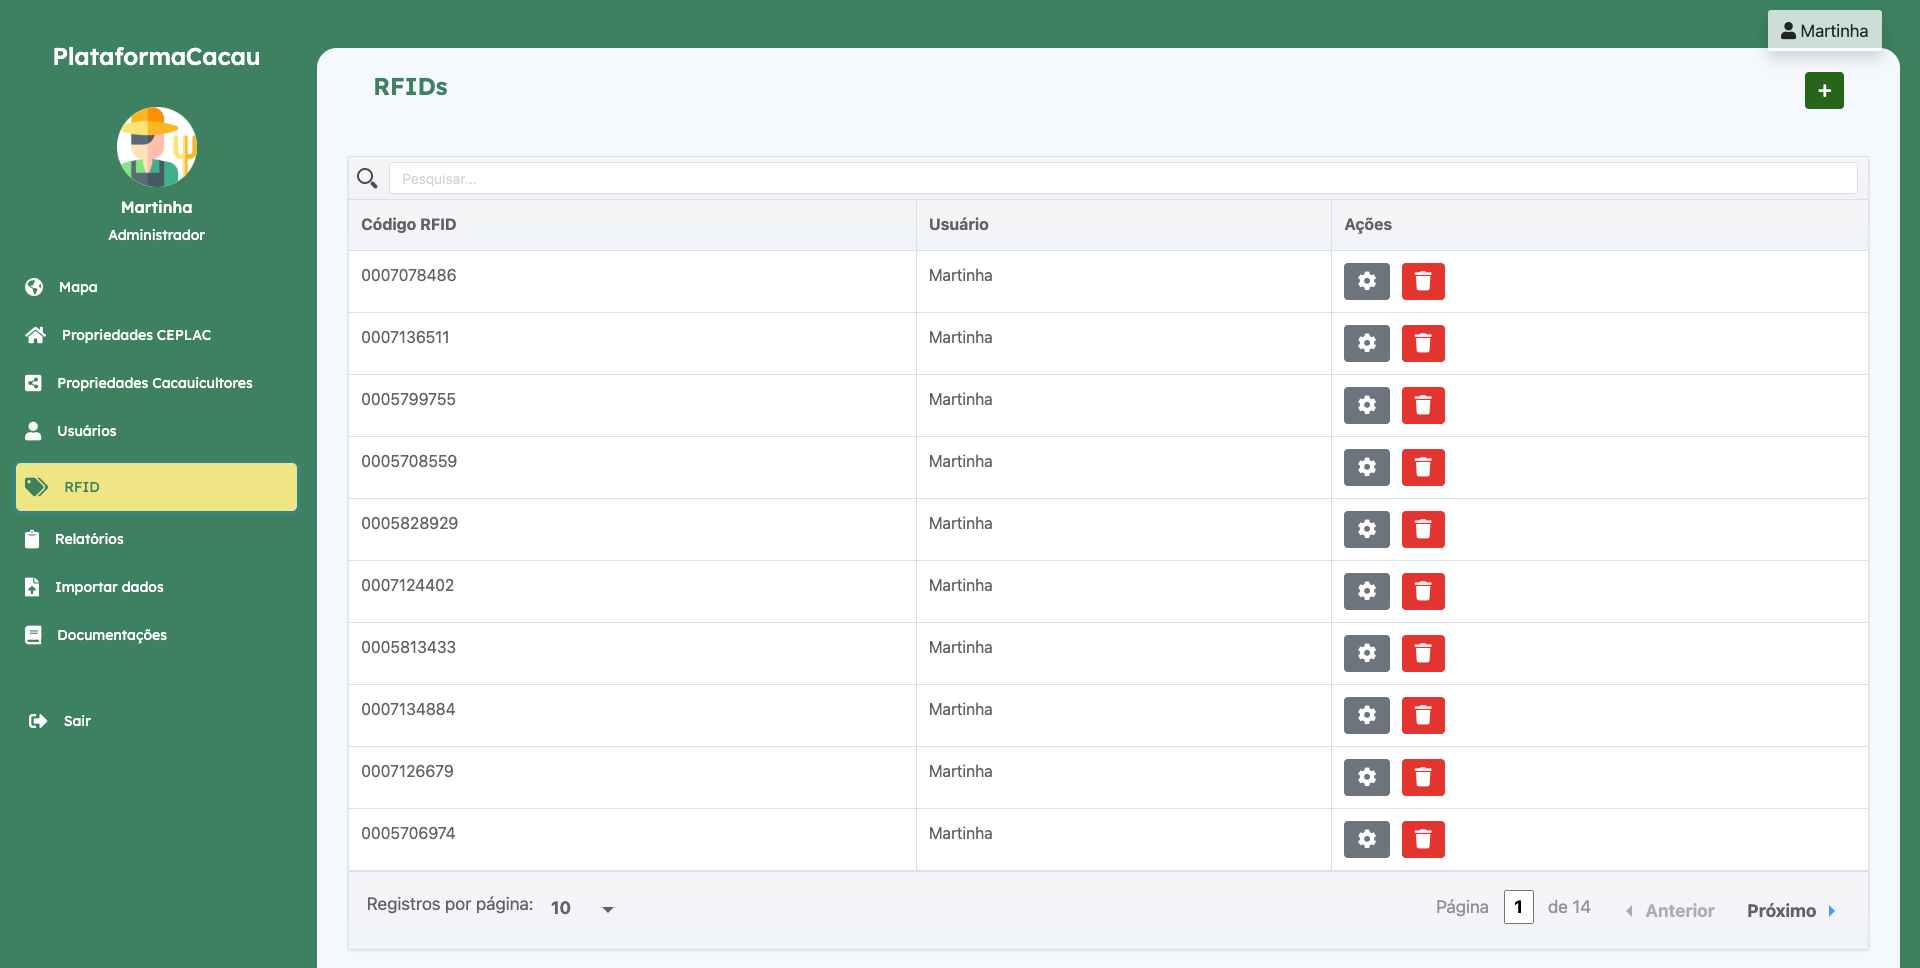
\includegraphics[width=\textwidth]{images/web/list-rfid.png}}
    \caption{Tela de listagem de RFIDs na plataforma web.}
    \label{fig:ListRfid}
\end{figure}

\subsubsection{Janela de Criação de Código RFID}
A Figura \ref{fig:CreateRfid} mostra a interface de cadastro de novos RFIDs, onde o gestor insere o código e outras informações necessárias para adicionar uma nova tag ao sistema.

\begin{figure}[H]
 \centering
 \frame{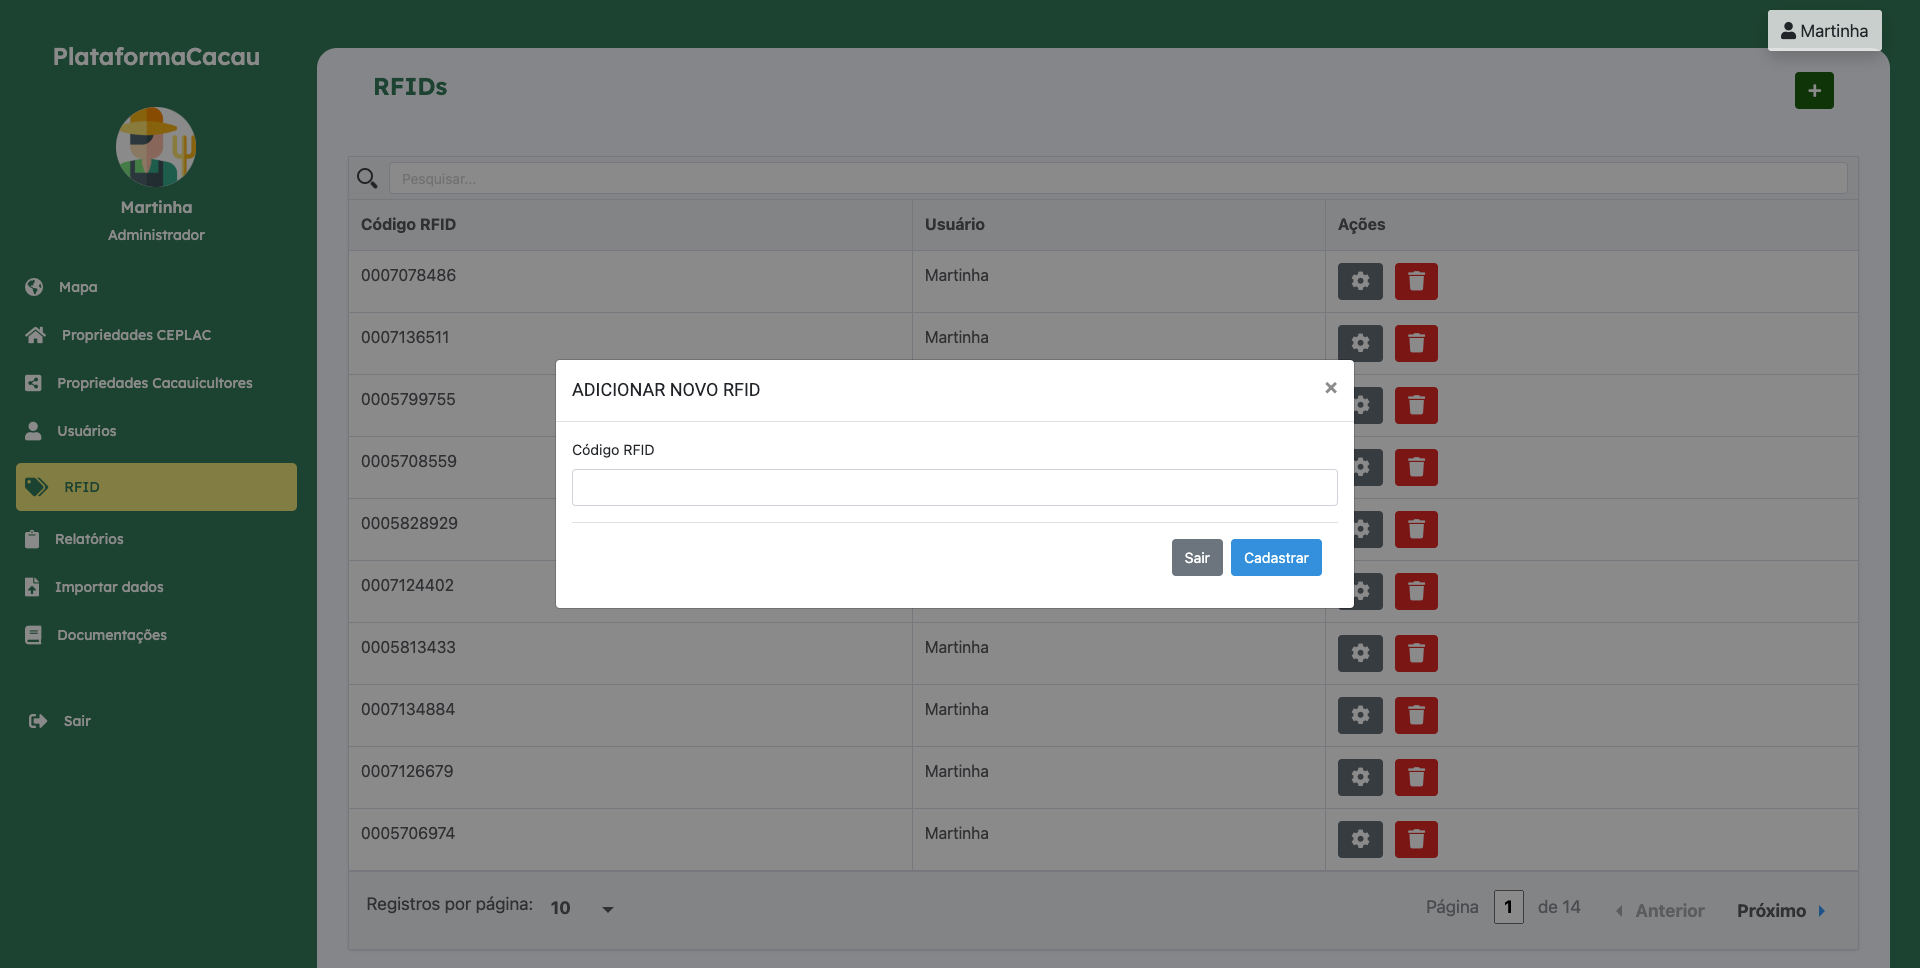
\includegraphics[width=\textwidth]{images/web/create-rfid.png}}
 \caption{Janela de criação de código RFID na plataforma web.}
 \label{fig:CreateRfid}
\end{figure}

\subsubsection{Janela de Atualização de Código RFID}
A Figura \ref{fig:UpdateRfid} representa a tela que permite ao gestor modificar as informações de um RFID existente, garantindo que o sistema reflita sempre as informações corretas.

\begin{figure}[H]
 \centering
 \frame{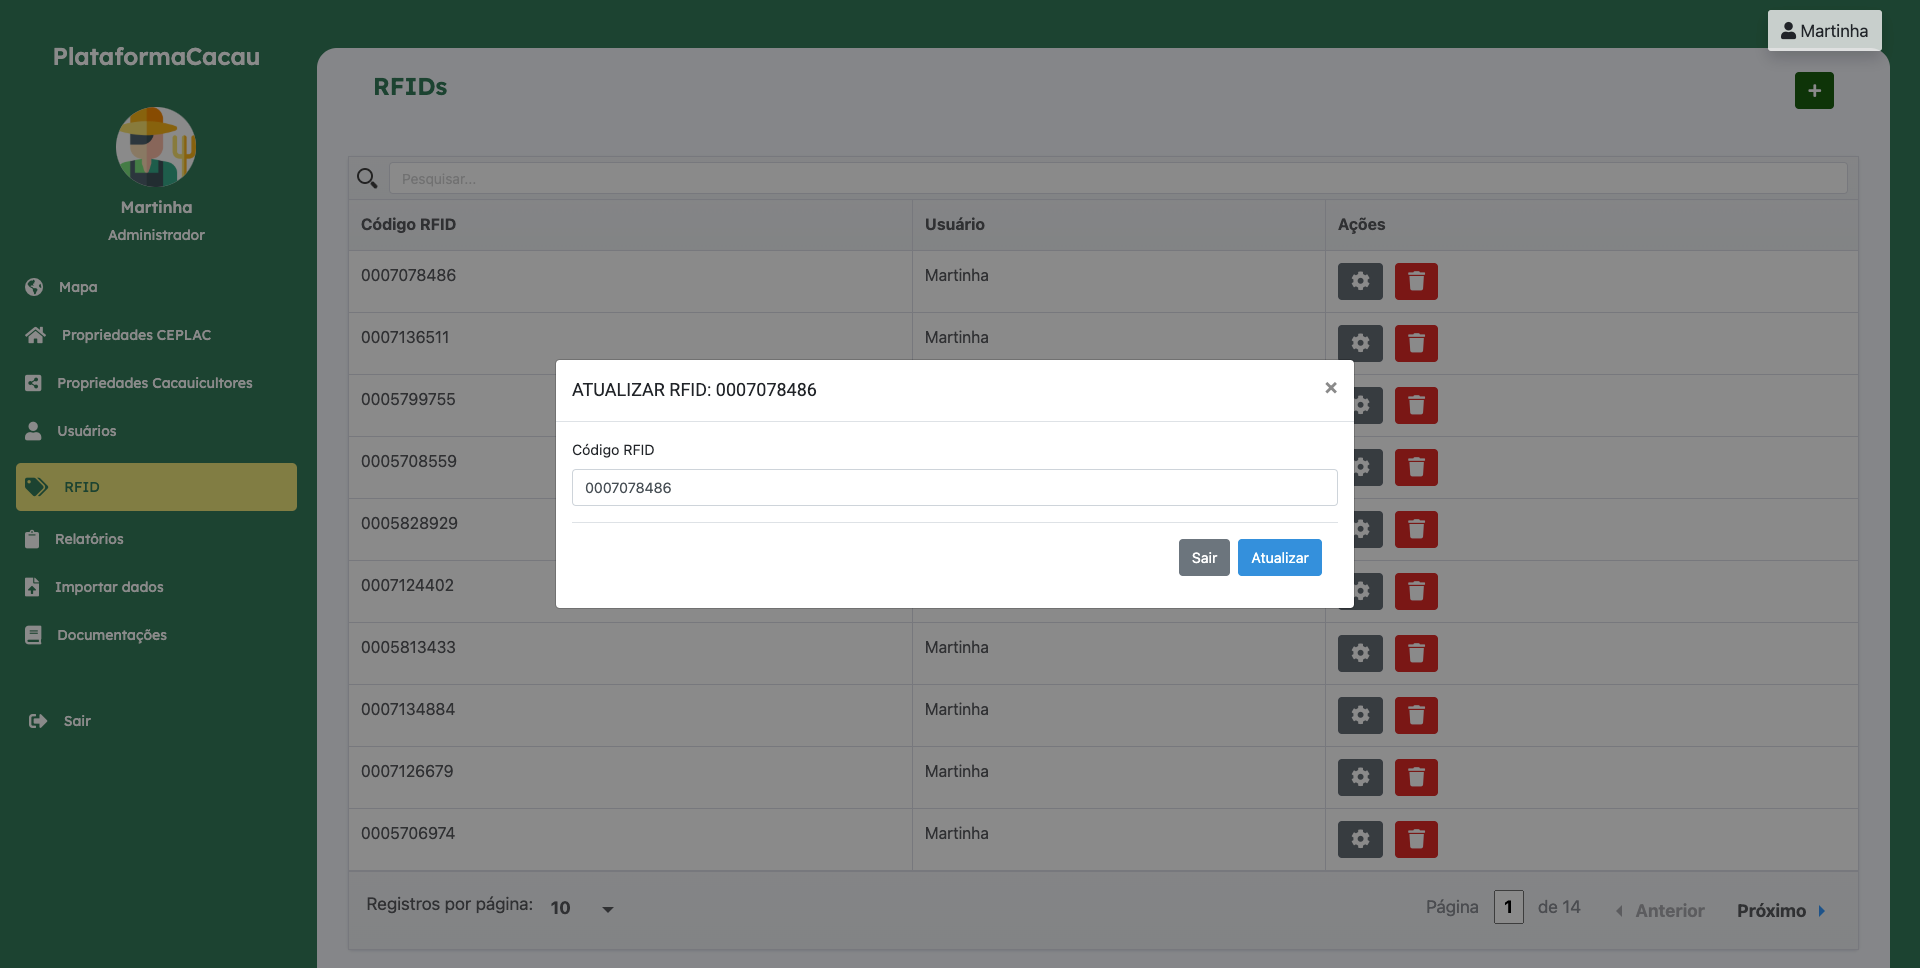
\includegraphics[width=\textwidth]{images/web/update-rfid.png}}
 \caption{Janela de atualização de código RFID na plataforma web.}
 \label{fig:UpdateRfid}
\end{figure}

\subsubsection{Tela de Listagem de Árvores}
A Figura \ref{fig:TreeList} exibe a lista completa de árvores cadastradas, com seus respectivos RFIDs, oferecendo uma visão geral organizada para o gestor.

\begin{figure}[H]
 \centering
 \frame{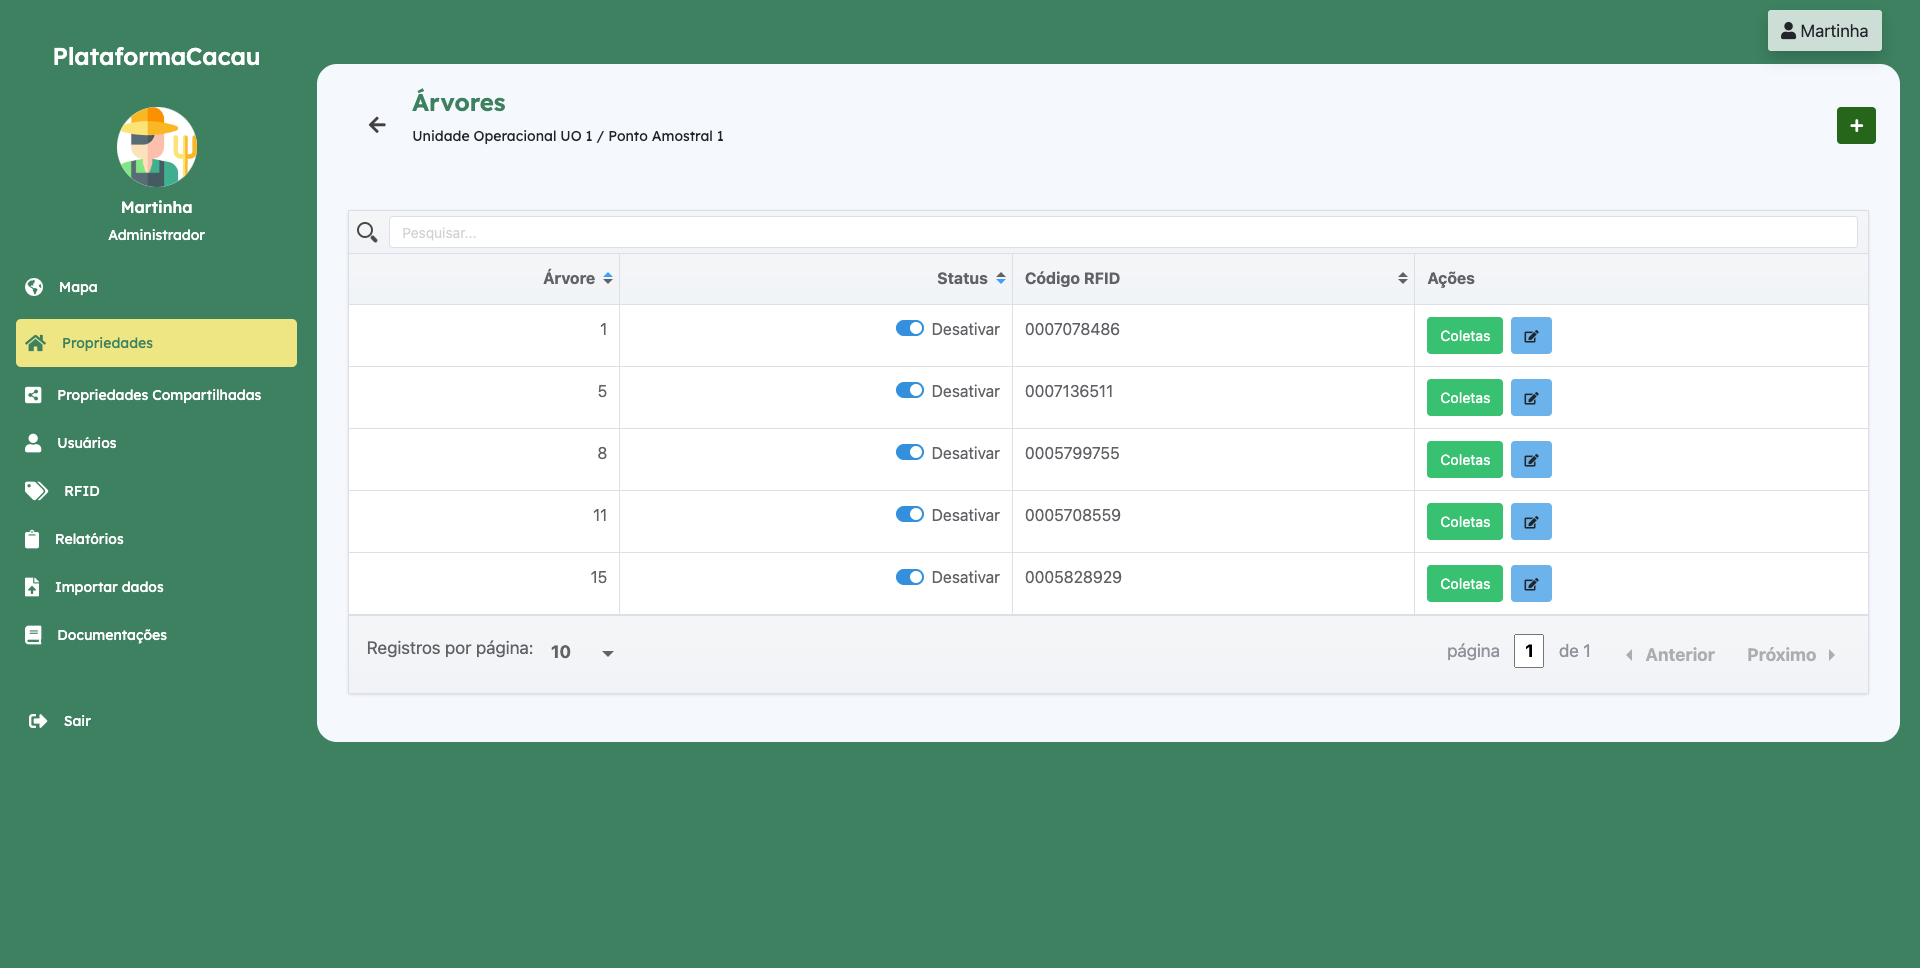
\includegraphics[width=\textwidth]{images/web/list-tree.png}}
 \caption{Tela de listagem de árvores na plataforma web.}
 \label{fig:TreeList}
\end{figure}

\subsubsection{Janela de atualização do código RFID da árvore}
A Figura \ref{fig:UpdateTreeRfid} representa a interface onde o gestor pode atualizar o código RFID vinculado a uma árvore específica, facilitando o gerenciamento e manutenção das tags associadas.

\begin{figure}[htb]
 \centering
 \frame{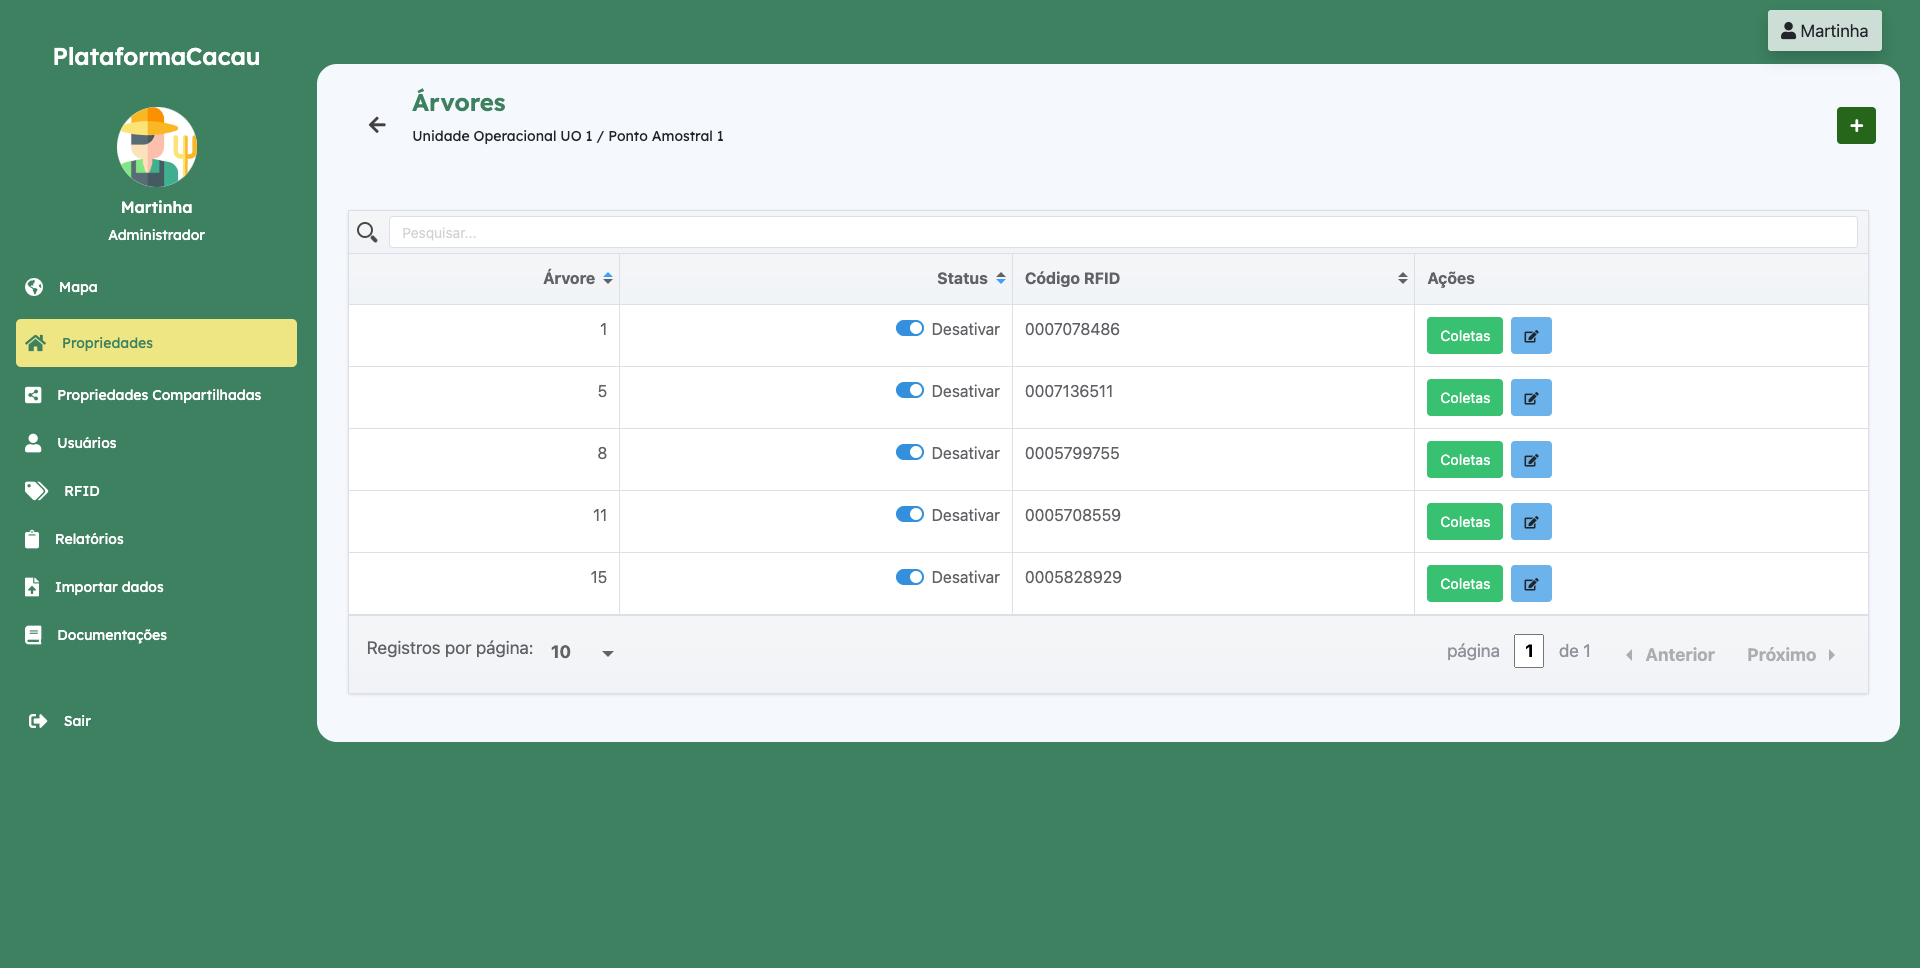
\includegraphics[width=\textwidth]{images/web/list-tree.png}}
 \caption{Janela de atualização do código RFID da árvore na plataforma web.}
 \label{fig:UpdateTreeRfid}
\end{figure}

\subsection{Imagens do Aplicativo Móvel}

\subsubsection{Telas de Listagem}
A Figura \ref{fig:ListScreens} inclui as telas de listagem de propriedades, unidades operacionais, áreas homogêneas, pontos amostrais e árvores, oferecendo uma navegação intuitiva para o coletor.

\begin{figure}[H]
    \centering
    \begin{minipage}[b]{0.30\textwidth}
        \centering
        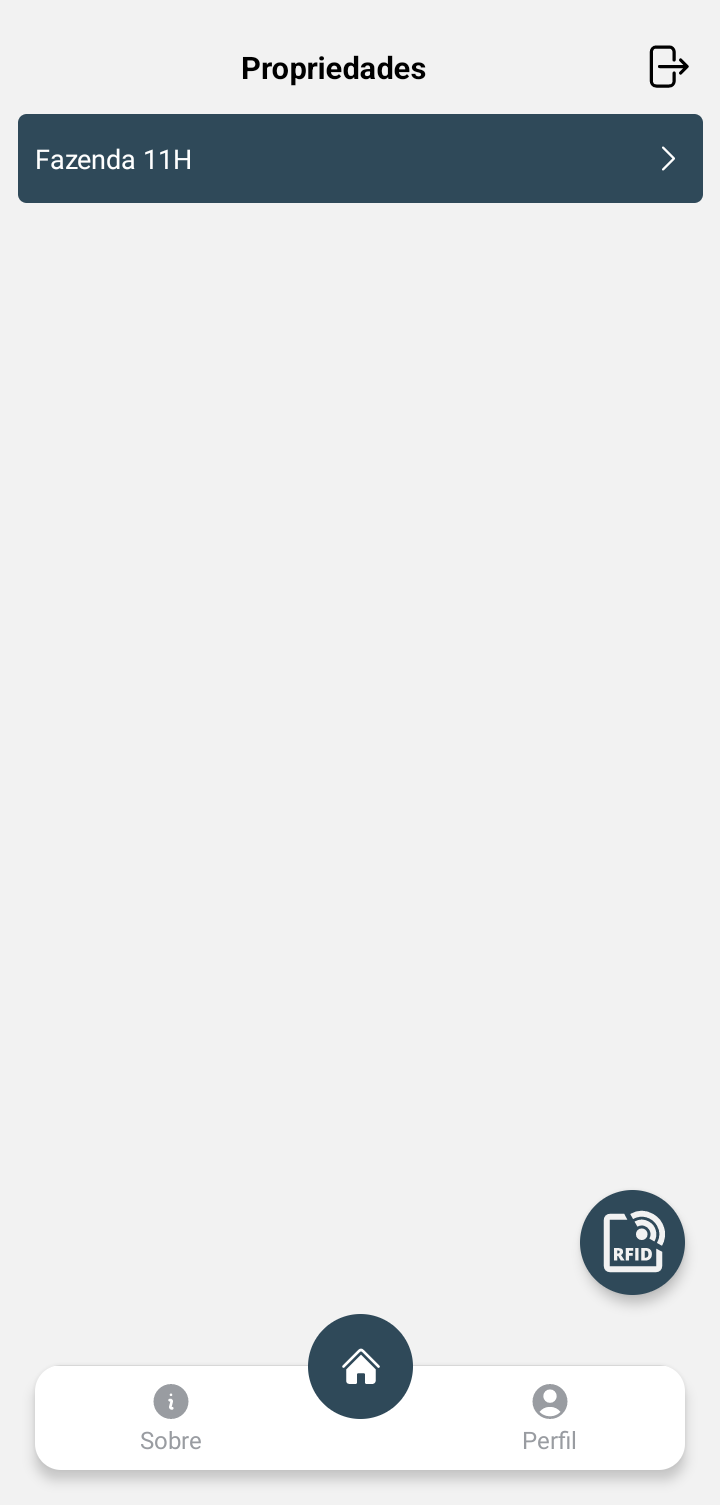
\includegraphics[width=\textwidth]{images/app/03-properties.png}
    \end{minipage}
    \hspace{3pt}
    \begin{minipage}[b]{0.30\textwidth}
        \centering
        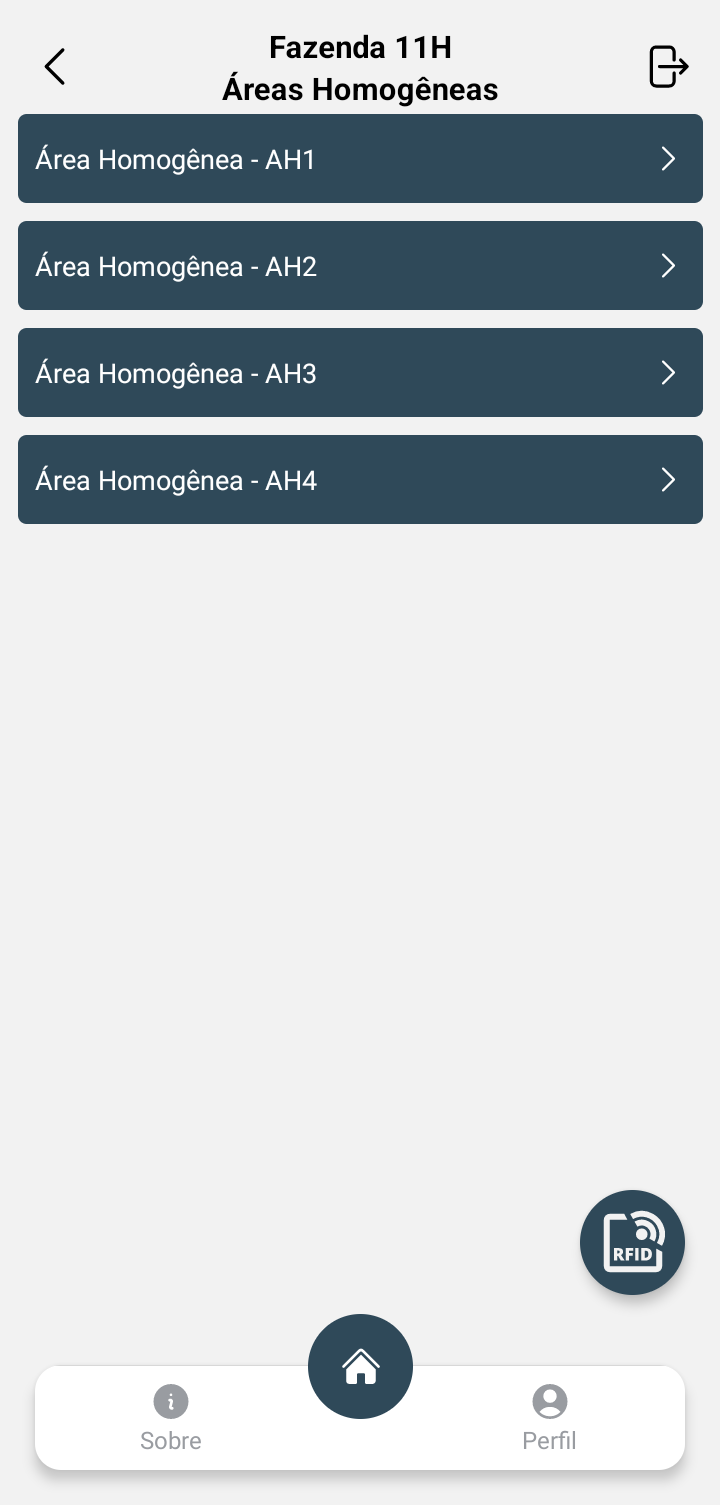
\includegraphics[width=\textwidth]{images/app/04-homogeneous-areas.png}
    \end{minipage}
    \hspace{3pt}
    \begin{minipage}[b]{0.30\textwidth}
        \centering
        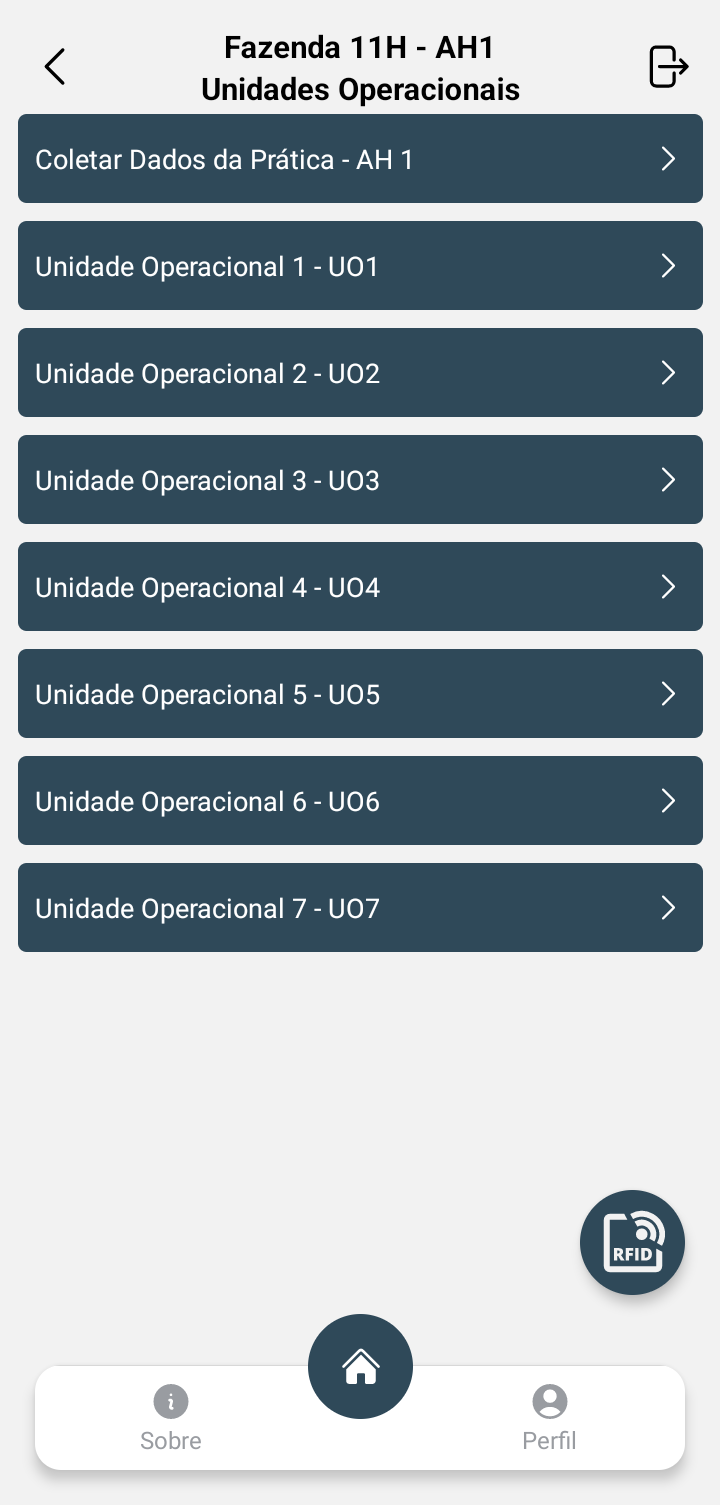
\includegraphics[width=\textwidth]{images/app/05-operational-units.png}
    \end{minipage}
    \hspace{3pt}
    \begin{minipage}[b]{0.30\textwidth}
        \centering
        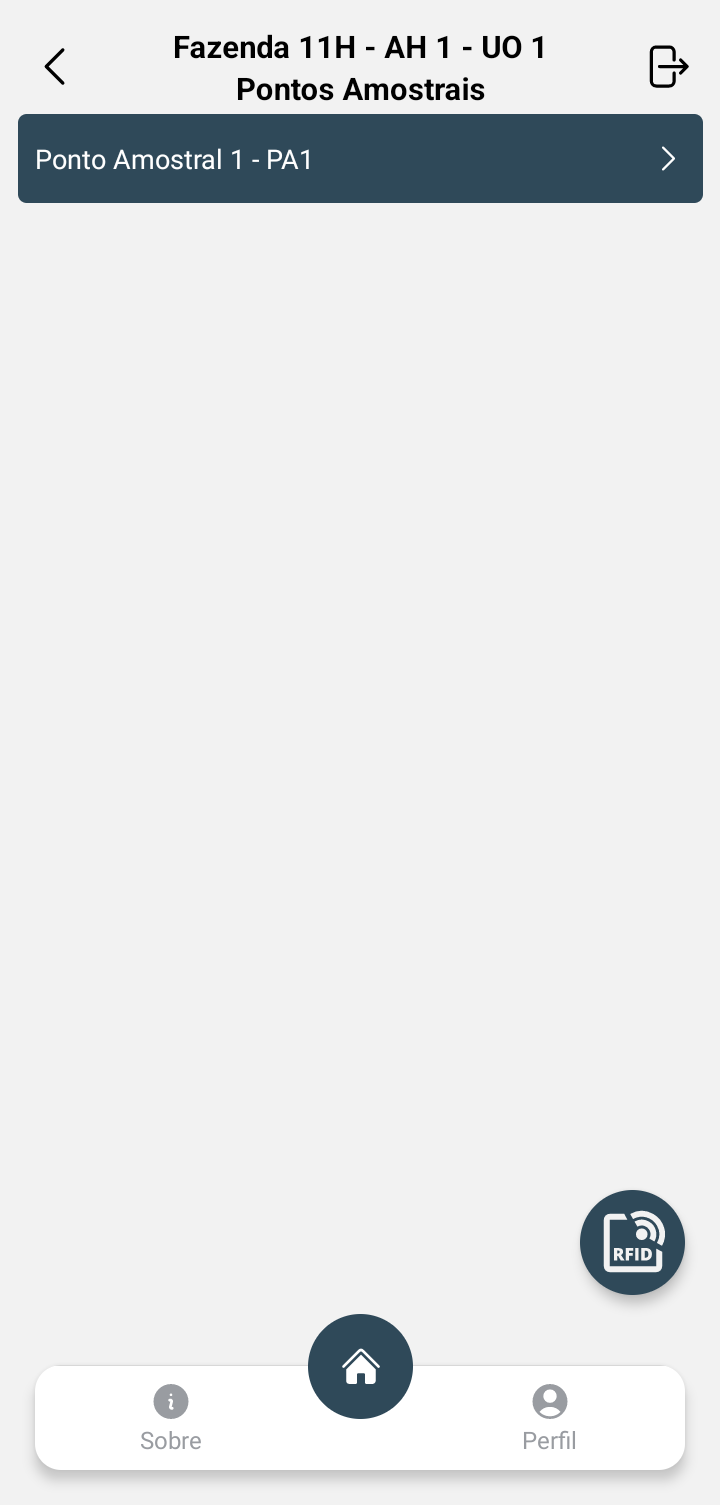
\includegraphics[width=\textwidth]{images/app/08-sampling-points.png}
    \end{minipage}
    \hspace{3pt}
    \begin{minipage}[b]{0.30\textwidth}
        \centering
        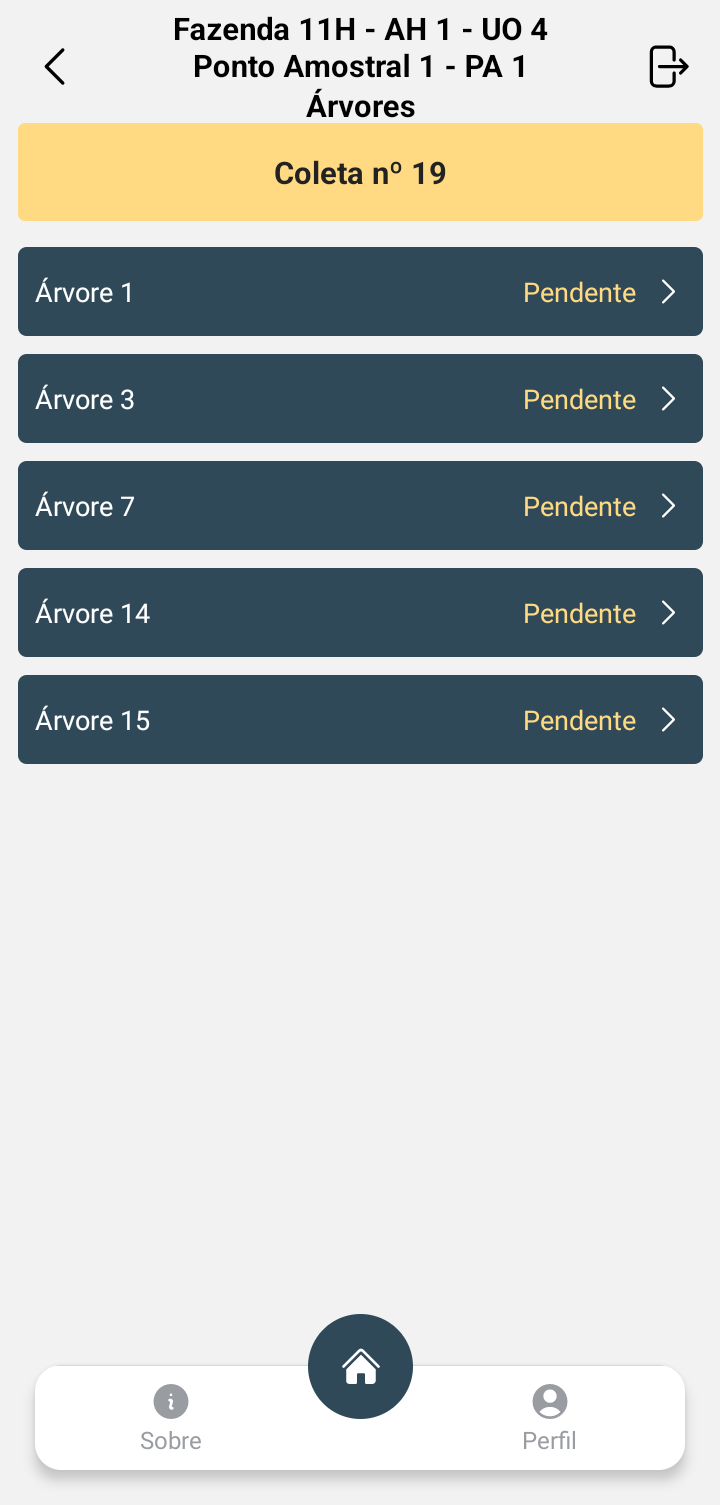
\includegraphics[width=\textwidth]{images/app/09-trees.png}
    \end{minipage}
    
    \caption{Telas de listagem do aplicativo móvel.}
    \label{fig:ListScreens}
\end{figure}

\subsubsection{Tela de Coleta dos Dados da Prática}
A Figura \ref{fig:PracticeDataScreen} representa a interface onde o coletor registra os dados gerais da área, incluindo condições de solo, presença de pragas, e outras informações relevantes sobre a saúde das plantas.

\begin{figure}[H]
    \centering
    \begin{minipage}[b]{0.30\textwidth}
        \centering
        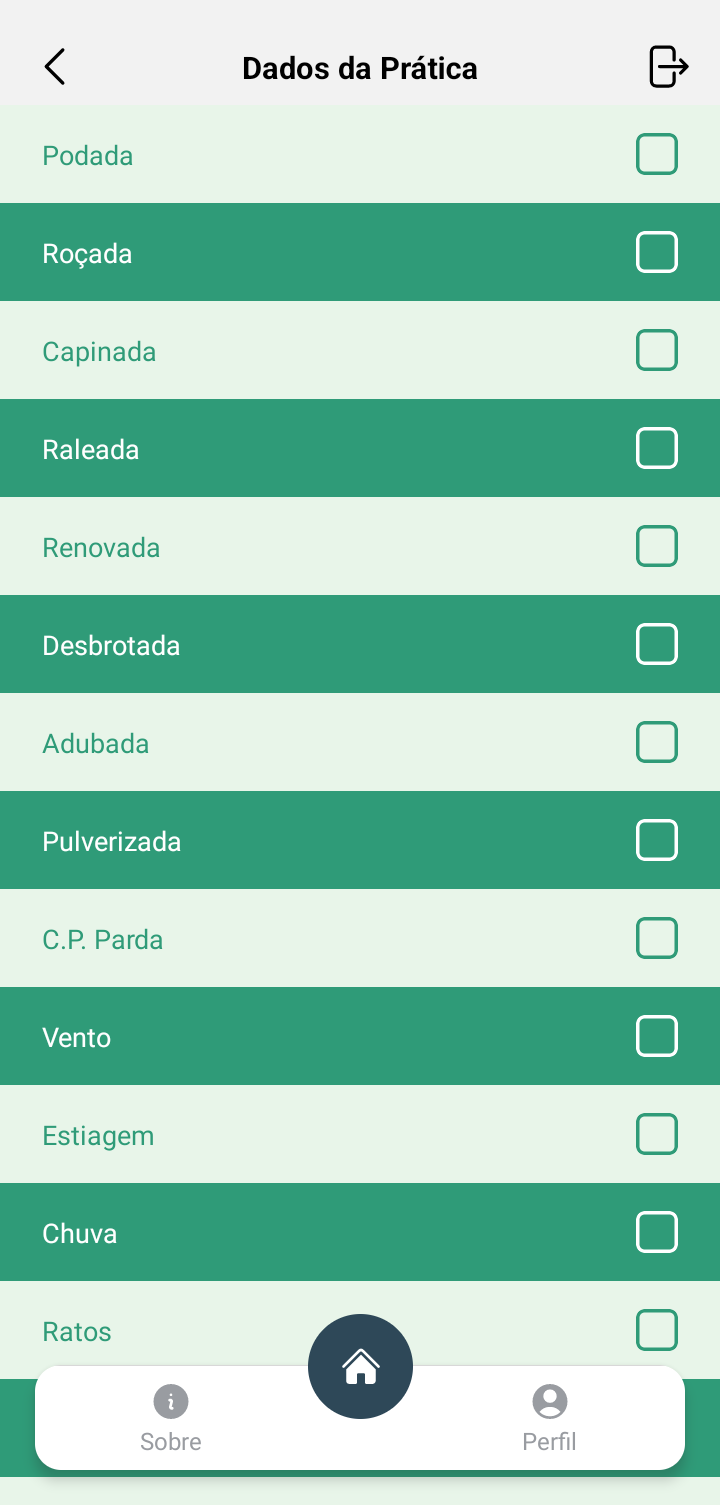
\includegraphics[width=\textwidth]{images/app/06-practice-data.png}
    \end{minipage}
    \hspace{5pt}
    \begin{minipage}[b]{0.30\textwidth}
        \centering
        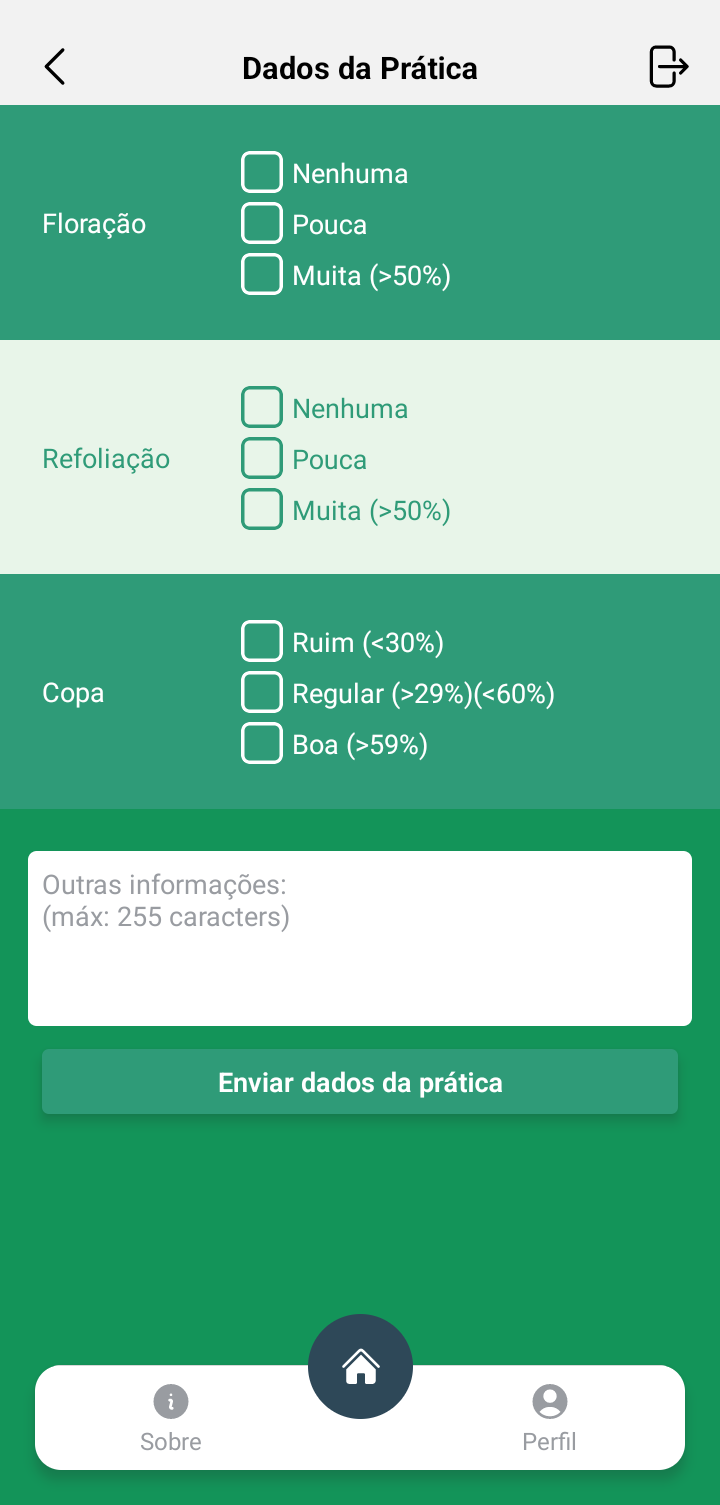
\includegraphics[width=\textwidth]{images/app/07-practice-data.png}
    \end{minipage}
    \hspace{5pt}
    
    \caption{Telas de coleta dos dados da prática no aplicativo móvel.}
    \label{fig:PracticeDataScreen}
\end{figure}

\subsubsection{Tela de Coleta dos Dados da Árvore}
A Figura \ref{fig:CollectDataScreen} representa a tela que permite ao coletor inserir dados específicos da árvore, como número de frutos e estágio de desenvolvimento, diretamente vinculado ao RFID da árvore.

\begin{figure}[H]
    \centering
    \begin{minipage}[b]{0.30\textwidth}
        \centering
        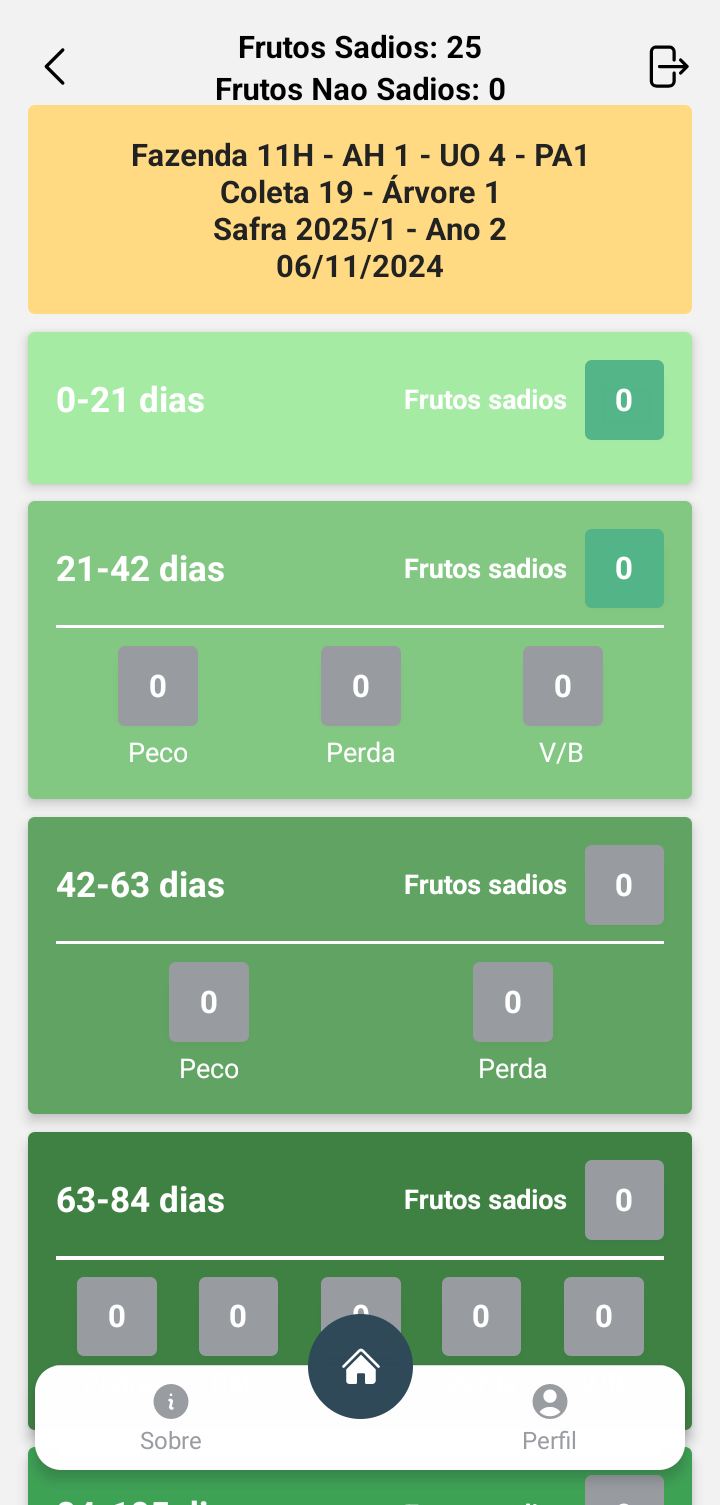
\includegraphics[width=\textwidth]{images/app/10-collect.png}
    \end{minipage}
    \hspace{3pt}
    \begin{minipage}[b]{0.30\textwidth}
        \centering
        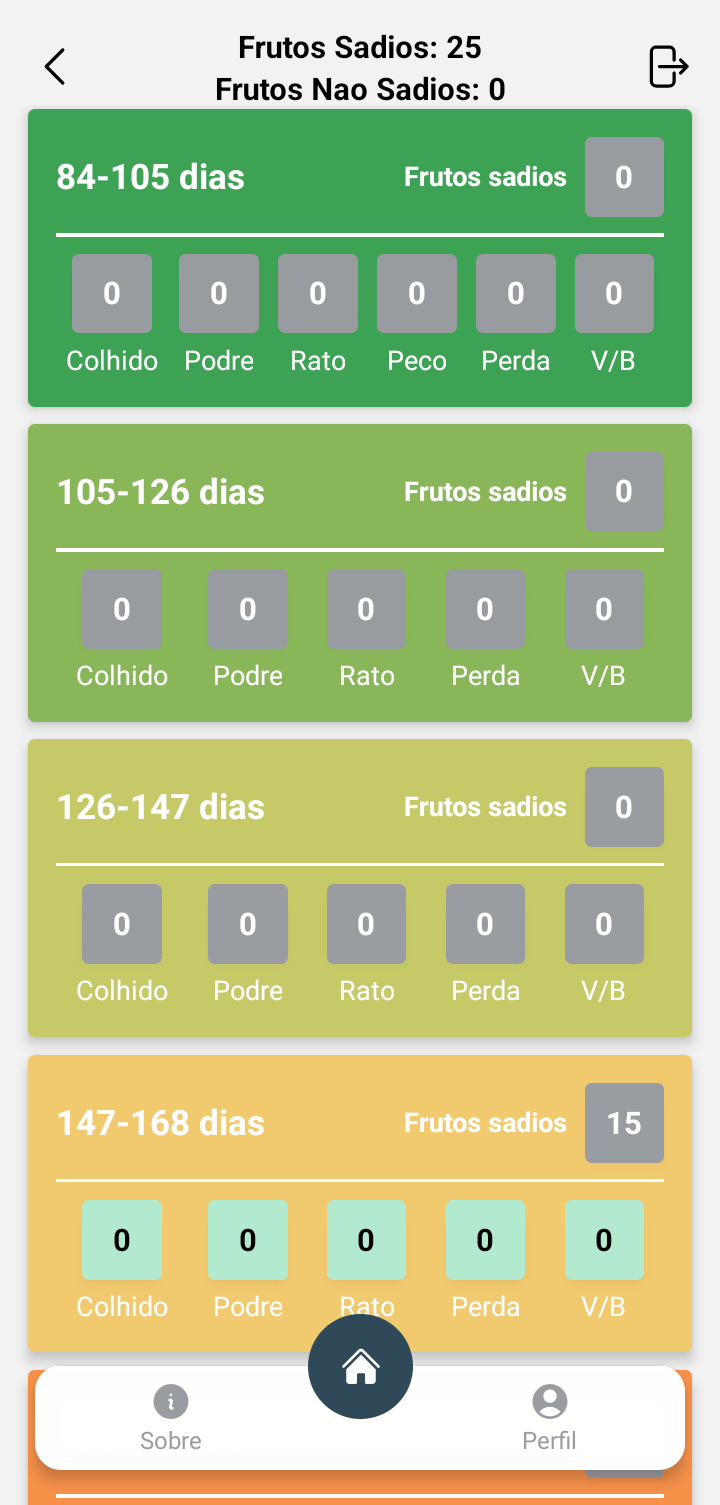
\includegraphics[width=\textwidth]{images/app/11-collect.png}
    \end{minipage}
    \hspace{3pt}
    \begin{minipage}[b]{0.30\textwidth}
        \centering
        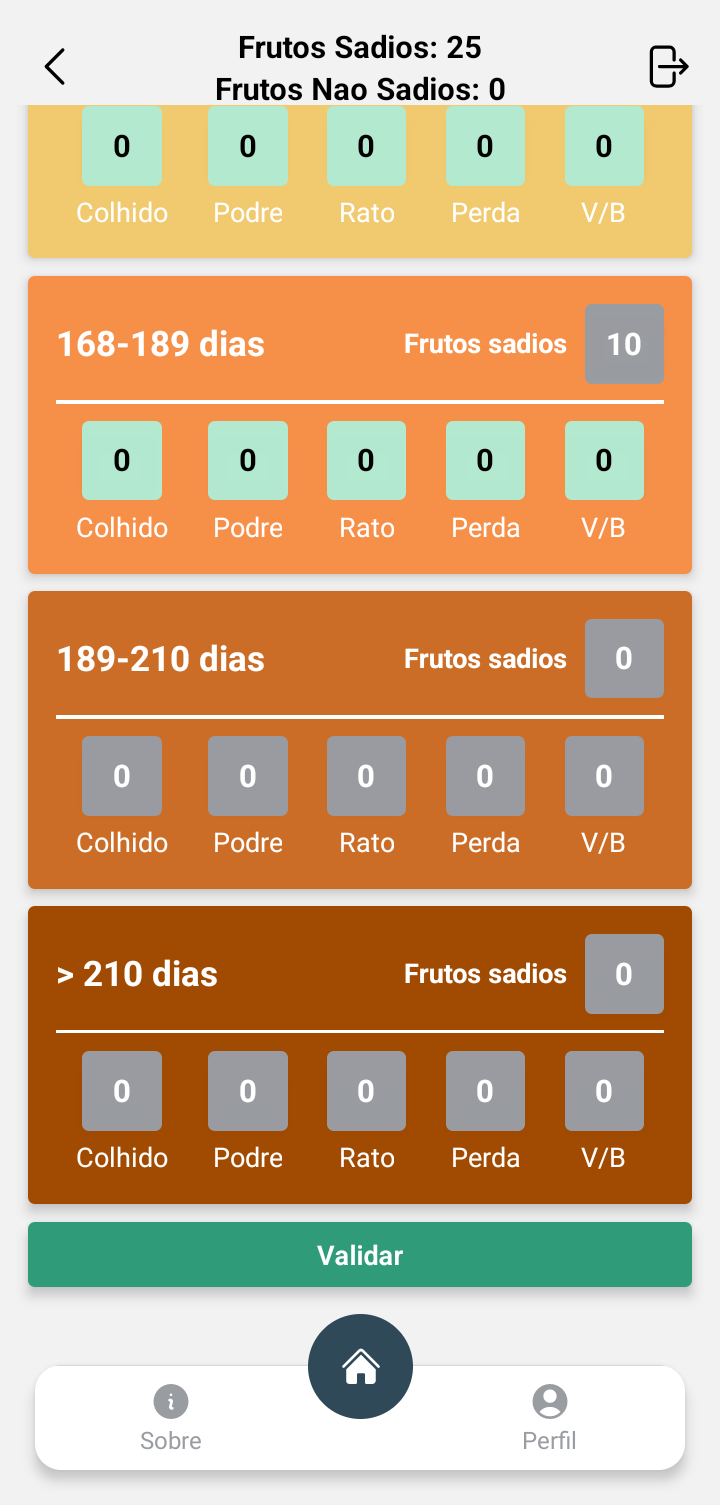
\includegraphics[width=\textwidth]{images/app/12-collect.png}
    \end{minipage}
    \hspace{3pt}
    
    \caption{Tela de coleta dos dados da árvore no aplicativo móvel.}
    \label{fig:CollectDataScreen}
\end{figure}


\subsection{Modal de Busca do RFID}
A Figura \ref{fig:RfidModal} representa o componente modal de busca de tags RFID que facilita a identificação das árvores durante a coleta, informando o RFID que está sendo pesquisado, agilizando o processo e minimizando erros de identificação. 

\begin{figure}[htb]
    \centering
    \begin{minipage}[b]{0.30\textwidth}
        \centering
        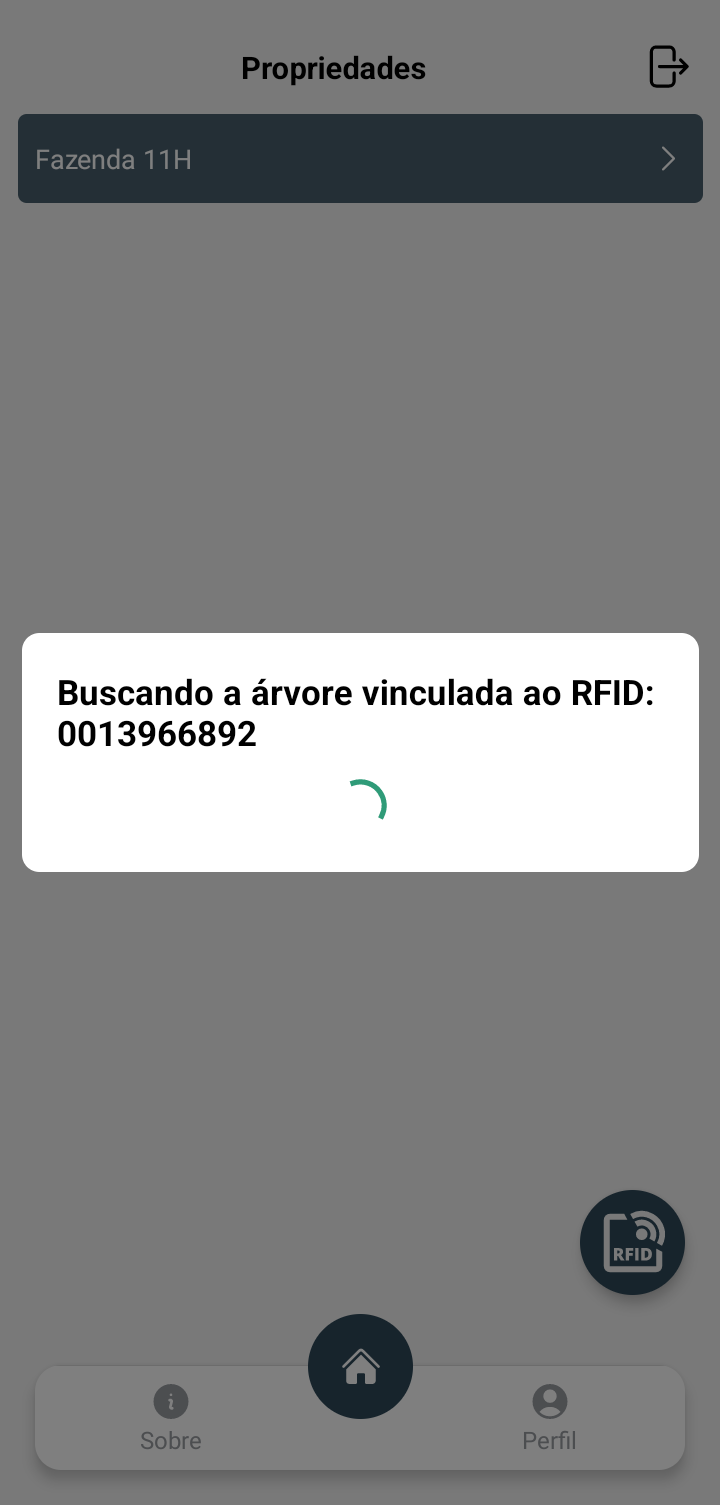
\includegraphics[width=\textwidth]{images/app/rfid-modal.png}
    \end{minipage}
    \caption{Modal de busca do RFID no aplicativo móvel.}
    \label{fig:RfidModal}
\end{figure}

Caso o ponto amostral já tenha sido visitado o aplicativo identifica este cenário e retorna uma mensagem informativa ao coletor. Este cenário pode ser visualizado na Figura \ref{fig:RfidSamplingPointVisitedMessage}

\begin{figure}[H]
    \centering
    \begin{minipage}[b]{0.30\textwidth}
        \centering
        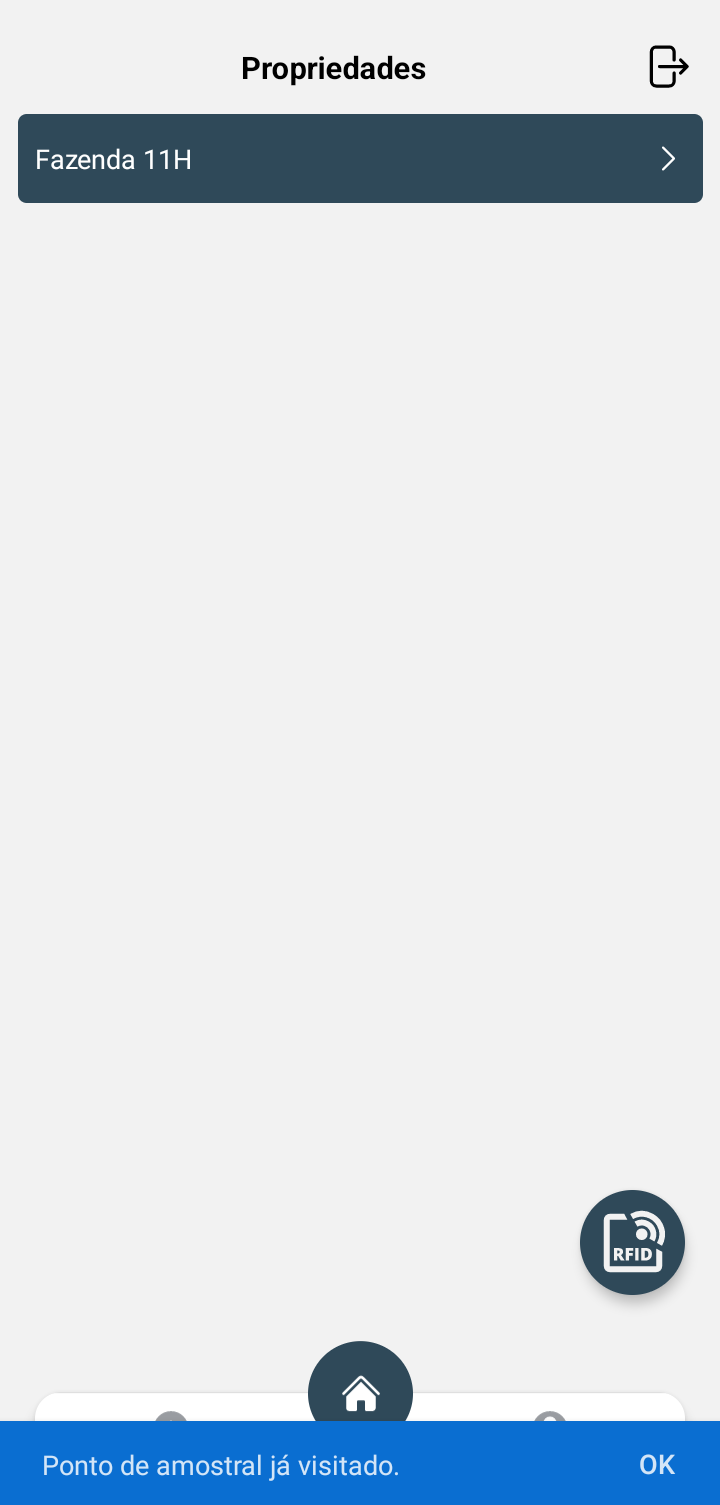
\includegraphics[width=\textwidth]{images/app/check-rfid-sp-visited.png}
    \end{minipage}
    \caption{Mensagem de busca do RFID indicando ponto amostral já visitado.}
    \label{fig:RfidSamplingPointVisitedMessage}
\end{figure}

\section{Estrutura de Dados e Funcionalidades da API}
Para garantir uma integração eficiente entre os diferentes módulos do ColetaCacau, foram implementadas funcionalidades adicionais na API e no banco de dados, descritas a seguir:

\subsection{Tabela de RFIDs Relacionada à Entidade de Árvores}
A tabela que armazena as tags RFID foi projetada para garantir a integridade dos dados e facilitar sua utilização no sistema, organizando as informações de forma clara e eficiente. Cada tag RFID está vinculada a uma árvore e pode também estar associada a um usuário responsável. Essa estrutura promove a rastreabilidade e consistência, essenciais para o funcionamento correto do ColetaCacau.

A principal característica dessa tabela é a unicidade dos códigos RFID. Cada código é único dentro do contexto da fazenda, isto é, só poderá existir um código RFID por fazenda mas, outras fazendas podem ter o mesmo código RFID. Além disso, as tags podem ser atualizadas ou desassociadas sem comprometer a integridade dos dados relacionados. Por exemplo, se uma fazenda ou usuário for excluído, a tag associada a ele não será removida, mas sim desvinculada, garantindo que os dados históricos sejam preservados.

A Figura \ref{fig:RfidTable} ilustra a organização e os relacionamentos dessa tabela no banco de dados, destacando como os registros de RFID interagem com outras entidades do sistema.

\begin{figure}[H]
    \centering
    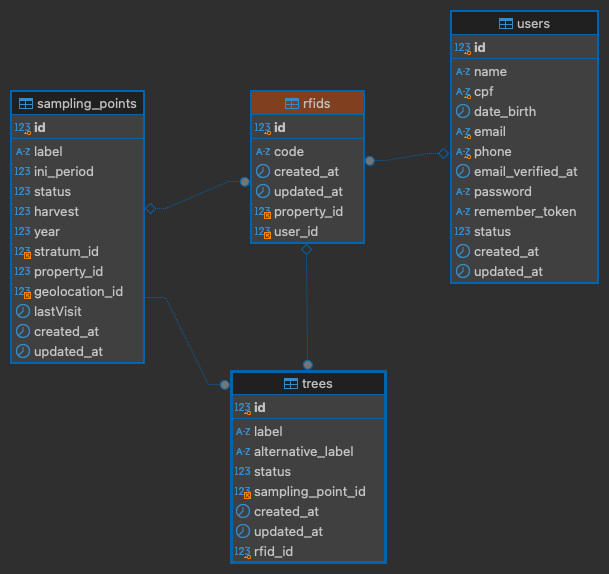
\includegraphics[width=0.8\textwidth]{images/database/rfid-table.png}
    \caption{Estrutura da tabela de RFIDs e seus relacionamentos no banco de dados.} \label{fig:RfidTable}
\end{figure}

\subsection{\textit{Endpoints} de Manipulação de RFIDs}
A API foi equipada com \textit{endpoints} específicos para realizar as operações de criação, atualização, listagem, visualização por ID, desassociação, exclusão e associação de RFIDs a uma árvore. Esses \textit{endpoints} oferecem flexibilidade e segurança no gerenciamento das tags, permitindo que o sistema se mantenha atualizado conforme as operações de campo evoluem.

\subsection{Exportação de Dados com RFID}
Foi incluído o campo de RFID relacionado a cada árvore na exportação de dados da coleta. Isso permite que os gestores tenham acesso a um relatório completo, incluindo a identificação única de cada árvore monitorada, o que facilita a análise de dados e o acompanhamento do progresso da safra ao longo do tempo.

\section{Discussão dos Testes e Resultados}
Os testes realizados demonstraram que o sistema ColetaCacau cumpre os requisitos de coleta de dados precisos e consistentes em campo, especialmente com a implementação de RFID e coleta \textit{offline}. As imagens apresentadas, tanto da plataforma web quanto do aplicativo móvel, reforçam a usabilidade e funcionalidade do sistema, demonstrando como cada funcionalidade contribui para a eficiência do trabalho dos coletores.

A redução significativa de tempo e a minimização de erros de identificação das árvores evidenciam os avanços obtidos com o uso de RFID, trazendo maior confiabilidade e eficiência à coleta de dados no campo. O sistema se mostra uma solução robusta para o monitoramento da safra de cacau, com potencial para ser expandido a outros contextos agrícolas no futuro.

\chapter{Discussões e Trabalhos Futuros}
Este projeto demonstrou a eficiência e a viabilidade do uso de RFID e coleta de dados \textit{offline} para otimizar o monitoramento da produção de cacau. No entanto, o potencial de evolução do ColetaCacau é vasto, e diversas melhorias e funcionalidades adicionais podem ser exploradas no futuro. As propostas a seguir apresentam possíveis avanços que poderiam enriquecer ainda mais a funcionalidade do sistema e expandir seu uso no setor agrícola.

\section{Automação de Geração e Gravação de Tags RFID}

A automação da geração de códigos para as tags RFID representa uma oportunidade estratégica para otimizar o processo de identificação e rastreamento de árvores e pontos amostrais. Com essa abordagem, é possível garantir um controle mais eficiente do inventário de tags, permitir sua reutilização e padronizar a estrutura dos códigos para facilitar a gestão.

\subsection{Padrão de Identificação para Tags RFID}

Para aprimorar a organização e o rastreamento, propõe-se a criação de um padrão estruturado que identifique informações relevantes, como o produtor, a fazenda, a unidade operacional (UO), o ponto amostral (PA) e a área homogênea (AH). Essa estrutura geraria um número único para cada tag RFID, permitindo uma identificação clara e inequívoca. Por exemplo:

\begin{itemize}
    \item \textbf{Formato do Código:} 
    \begin{center}
    [PROPRIEDADE]-[AH]-[UO]-[PA]-[ID\_Árvore]
    \end{center}
    \item \textbf{Exemplo:} 
    \begin{center}
    1234-5678-01-002-003
    \end{center}
\end{itemize}

\noindent Onde:
\begin{itemize}
    \item \textbf{1234:} Identificador único da propriedade.
    \item \textbf{5678:} Identificador único da Área Homogênea.
    \item \textbf{01:} Unidade operacional específica.
    \item \textbf{002:} Número do ponto amostral.
    \item \textbf{003:} Identificador da árvore.
\end{itemize}

Essa padronização permite que o sistema associe rapidamente uma tag RFID às informações da árvore ou ponto amostral, facilitando a consulta e reduzindo erros durante o processo de coleta.

\subsection{Implementação}

Na interface de gestão de tags RFID, seria desenvolvido um módulo para:
\begin{enumerate}
    \item \textbf{Geração Automática de Códigos:}
    Um algoritmo incorporaria o padrão de identificação descrito acima, garantindo que cada tag gerada tenha um número exclusivo e seguindo a estrutura definida.

    \item \textbf{Gravação Automática de Tags:}
    A integração com um gravador RFID permitiria que os códigos gerados fossem diretamente gravados nas tags. Esse processo agilizaria a preparação de tags para uso em campo, eliminando etapas manuais.

    \item \textbf{Controle de Estoque e Reutilização de Tags:}
    Um sistema de inventário monitoraria o uso das tags RFID, identificando aquelas que já foram desativadas ou não estão mais em uso. Essas tags poderiam ser reprogramadas com novos códigos, promovendo economia e sustentabilidade.
\end{enumerate}

\subsection{Benefícios}

\begin{itemize}
    \item \textbf{Eficiência Operacional:} O padrão padronizado e a automação da gravação de tags reduzem o tempo gasto no gerenciamento e na identificação manual.
    \item \textbf{Rastreabilidade:} A estrutura do código fornece informações detalhadas, permitindo um rastreamento claro e completo.
    \item \textbf{Sustentabilidade:} A reutilização de tags diminui os custos operacionais e os resíduos gerados.
\end{itemize}

Essa implementação simplifica o processo de gestão de tags RFID, tornando o sistema mais eficiente, organizado e adaptável às necessidades do ColetaCacau.

\section{Integração com Sensores IoT para Monitoramento Ambiental}
Uma evolução natural do ColetaCacau é integrar o sistema a sensores IoT (Internet das Coisas) que monitoram em tempo real as condições ambientais da lavoura, como umidade do solo, temperatura, luminosidade e índices de chuva. Esses dados complementariam as informações da coleta, fornecendo aos gestores uma visão ainda mais detalhada das condições de crescimento das plantas. Além disso, alertas automáticos poderiam ser configurados para notificar os coletores e gestores sobre mudanças ambientais que possam afetar a produção de cacau, permitindo ações preventivas.

\textbf{Implementação:} Sensores de baixo custo e de fácil instalação poderiam ser distribuídos pela área de plantio, enviando dados diretamente para o aplicativo ou plataforma web do ColetaCacau via redes de longo alcance como \textit{LoRaWAN} ou \textit{Sigfox}. Esses dados poderiam ser integrados ao banco de dados do sistema para uma análise conjunta com as informações da coleta.

\section{Análise Preditiva com Machine Learning}
Uma proposta inovadora para o ColetaCacau é incorporar algoritmos de Machine Learning para análise preditiva, ajudando a antecipar potenciais problemas e tendências na produção. Com a coleta contínua de dados das árvores e, possivelmente, das condições ambientais, modelos preditivos poderiam ser treinados para identificar padrões e prever eventos, como:

\begin{itemize} 
    \item Risco de doenças e pragas baseado em padrões de coleta e condições ambientais.
    
    \item Estimativa de produção com base em históricos de coleta e desenvolvimento dos frutos.
\end{itemize}

\textbf{Implementação:} Algoritmos de Machine Learning, como redes neurais ou árvores de decisão, poderiam ser treinados usando dados históricos do \textbf{ColetaCacau}. A análise preditiva seria visualizada na plataforma web, oferecendo aos gestores uma ferramenta poderosa para tomada de decisão.

\section{Integração de Gravador RFID}
Para potencializar ainda mais o uso de RFID, a integração de um gravador RFID no sistema é uma opção promissora. Com isso, o sistema permitiria não apenas a leitura, mas também a gravação de informações nas tags RFID, facilitando o reaproveitamento de tags e a criação de fluxos de coleta mais integrados.

\textbf{Implementação:} Um gravador RFID seria integrado à plataforma para permitir a gravação e atualização das tags diretamente no campo ou na unidade de processamento. Esse fluxo adicional de escrita e reprogramação das tags contribuiria para reduzir o custo com novas etiquetas, tornando a operação mais eficiente e sustentável.


\section{Conclusão}
Os trabalhos futuros descritos apresentam um panorama de possíveis evoluções para o ColetaCacau, expandindo suas funcionalidades e seu impacto na agricultura de precisão. Desde o uso de \textbf{IoT} e \textbf{análise preditiva} até a integração de gravador RFID e automação de geração de tags, essas propostas exploram novas fronteiras tecnológicas que podem transformar o sistema em uma plataforma de monitoramento agrícola ainda mais abrangente e inovadora. Essas melhorias não só fortaleceriam a eficiência e a precisão do sistema, mas também aumentariam seu valor agregado, beneficiando diretamente os coletores, gestores e o consumidor final.

Com a implementação dessas propostas, o ColetaCacau tem o potencial de se tornar uma referência em tecnologia agrícola, liderando o caminho para uma produção mais eficiente, sustentável e conectada.

% ----------------------------------------------------------
% Finaliza a parte no bookmark do PDF
% para que se inicie o bookmark na raiz
% e adiciona espaço de parte no Sumário
% ----------------------------------------------------------
\phantompart

% ---
% Conclusão
% ---
%\chapter{Conclusão}
% ---

% ----------------------------------------------------------
% ELEMENTOS PÓS-TEXTUAIS
% ----------------------------------------------------------
\postextual
% ----------------------------------------------------------

% ----------------------------------------------------------
% Referências bibliográficas
% ----------------------------------------------------------
\bibliography{inputs/refs}

% ----------------------------------------------------------
% Glossário
% ----------------------------------------------------------
%
% Consulte o manual da classe abntex2 para orientações sobre o glossário.
%
%\glossary

%% ----------------------------------------------------------
% Apêndices
% ----------------------------------------------------------

% ---
% Inicia os apêndices
% ---
\begin{apendicesenv}

% Imprime uma página indicando o início dos apêndices
\partapendices

% ----------------------------------------------------------
\chapter{Quisque libero justo}
% ----------------------------------------------------------

\lipsum[50]

% ----------------------------------------------------------
\chapter{Nullam elementum urna vel imperdiet sodales elit ipsum pharetra ligula
ac pretium ante justo a nulla curabitur tristique arcu eu metus}
% ----------------------------------------------------------
\lipsum[55-57]

\end{apendicesenv}
% ---

%% ----------------------------------------------------------
% Anexos
% ----------------------------------------------------------

% ---
% Inicia os anexos
% ---
\begin{anexosenv}

% Imprime uma página indicando o início dos anexos
\partanexos
% ---
\begin{comment}
    \chapter{Detalhes do desenvolvimento da aquisição da imagem da tábua de corte}
\label{chap:anexos}

Para a aplicação da câmera, duas classes principais foram criadas: \textit{CameraShow} e \textit{CanvasShow}.

A \textit{CameraShow} é uma extensão da classe \textit{AppCompatActivity} fornecida pela Google para a criação de \textit{views}. Sua estrutura consiste dos componentes \textit{RelativeLayout}, \textit{TextureView} e \textit{Button}, descritos mais a frente. Enquanto que a classe \textit{CanvasShow} é uma extensão da classe \textit{View}, onde seu principal objetivo é a criação de um \textit{Frame} (moldura) dinâmico, a partir da área de exibição da câmema, utilizando a sobreposição do método \textit{onDraw} da classe \textit{View}, para posterior aquisição da imagem.

A geração dinâmica do \textit{Frame} possui como entrada a área de resolução da câmera com ofuscamento de 38\% da altura. Essa característica foi obtida de forma empírica, devido aos testes realizados após a aquisição da imagem em dispositivos de diferentes resoluções.

Foi necessário a utilização de recursos fornecidos pelo SO Android, por exemplo, a utilização da câmera e do armazenamento interno, e por exigência, o recurso só é fornecido mediante permissão do usuário. Portanto, algumas permissões de uso foram definidas no arquivo \textit{manifest}, que contém informações essenciais sobre a aplicação, e novamente de forma explicita no código, quando necessário a sua utilização.

\begin{figure}[htbp!]
  \centering
  \caption{Fluxo básico das funcionalidades da classe \textit{CameraShow}.}
  \includegraphics[width=1\textwidth]{figs/fluxograma_camera.png}
    \legend{Fonte: Elaborada pelo autor}
    \label{fig:fluxograma_camerashow}
\end{figure}

A Figura \ref{fig:fluxograma_camerashow} apresenta, resumidamente, as operações realizadas na classe \textit{CameraShow}. A seguir, cada etapa será explicada detalhadamente.

\begin{enumerate}
    \item Inicialização: Nele está contido toda operação realizada pelo construtor da classe, preparando o ambiente para configuração e abertura da câmera, para posterior aquisição da imagem. Em suma, ele integra os recursos fornenecidos pelos componentes, controles e \textit{Frame}.
    \begin{itemize}
        \item Componentes: Objetos exibidos durante a execução da câmera. Entre eles:
        \begin{itemize}
            \item \textit{RelativeLayout}: Componente que determina como será organizado e posicionado os demais objetos contidos nele.
            \item \textit{TextureView}: Área para apresentação de uma previsualização instantânea do cenário registrado pela câmera.
            \label{ite:texture_view}
            \item \textit{Button}: Botão exibido na interface para captura de uma imagem.
        \end{itemize}
        
        \item Controles: Contém métodos de pré-configuração da câmera, monitorando a forma que é executada, exibida ou tratamento de possíveis exceções ocorridas durante o acesso. Entre eles:
        \begin{itemize}
            \item \textit{initStateCallBack}: Método utilizado para indicar o estado da câmera, ou seja, quando é aberta ou quando ocorreu um erro durante o acesso.
            \item \textit{initSurfaceTextureListener}: Método que prepara a previsualização que será exibida em \textit{TextureView}.
        \end{itemize}
        
        \item \textit{Frame}: Criação da moldura que será apresentada na tela do dispositivo para auxiliar na aquisição da imagem.
    \end{itemize}
    
    \item Permissão: Após a inicialização da classe, é verificado se a aplicação possui as permissões do usuário para prosseguir com a execução.
    
    \item Execução paralela: Caso tudo esteja certo, um novo \textit{thread} é criado (divisão do processo) para utilização da câmera de forma paralela, aliviando a \textit{thread} principal do sistema. Alguns controles que liberam ou retomam o uso da câmera ou interrompem o \textit{thread} por um breve momento também estão presentes nessa etapa. Aqui, duas situações podem ocorrer com frequência: a câmera pode sofrer alterações, por exemplo, de orientação; ou o botão para aquisição da imagem pode ser acionado.
    \begin{itemize}
        \item Atualização da exibição: Devido a etapa de inicialização, alguns componentes que monitoram o uso da câmera pode alerta para alterações realizadas na mesma, como por exemplo, a mudança de horizontal para vertical. Sendo assim, um reajuste é necessário, sendo realizado por um método específico nomeado como \textit{update}.
        \item Aquisição da imagem: Caso o botão da câmera seja acionado, um método de captura da imagem registra o cenário da câmera, congelando a exibição por um breve momento, e depois a libera, devolvendo o controle. Com a captura, uma mudança no estado da câmera foi notado (congelando a exibição), sendo assim, uma atualização da exibição também é realizada nesse momento.
    \end{itemize}
    
    \item Encerramento: Etapa trivial mas de grande importância. Por boas práticas, todo recurso solicitado ou utilizado devem ser liberados, ocorrendo aqui.
\end{enumerate}

Em Figura \ref{fig:tela_captura} é observado o resultado final obtido com o desenvolvimento da câmera.

% ---


\end{comment}


\end{anexosenv}

%---------------------------------------------------------------------
% INDICE REMISSIVO
%---------------------------------------------------------------------
\phantompart
\printindex
%---------------------------------------------------------------------

\end{document}
